\documentclass[a4paper]{book}
\usepackage{makeidx}
\usepackage{natbib}
\usepackage{graphicx}
\usepackage{multicol}
\usepackage{float}
\usepackage{listings}
\usepackage{color}
\usepackage{ifthen}
\usepackage[table]{xcolor}
\usepackage{textcomp}
\usepackage{alltt}
\usepackage{ifpdf}
\ifpdf
\usepackage[pdftex,
            pagebackref=true,
            colorlinks=true,
            linkcolor=blue,
            unicode
           ]{hyperref}
\else
\usepackage[ps2pdf,
            pagebackref=true,
            colorlinks=true,
            linkcolor=blue,
            unicode
           ]{hyperref}
\usepackage{pspicture}
\fi
\usepackage[utf8]{inputenc}
\usepackage{mathptmx}
\usepackage[scaled=.90]{helvet}
\usepackage{courier}
\usepackage{sectsty}
\usepackage[titles]{tocloft}
\usepackage{doxygen}
\lstset{language=C++,inputencoding=utf8,basicstyle=\footnotesize,breaklines=true,breakatwhitespace=true,tabsize=8,numbers=left }
\makeindex
\setcounter{tocdepth}{3}
\renewcommand{\footrulewidth}{0.4pt}
\renewcommand{\familydefault}{\sfdefault}
\hfuzz=15pt
\setlength{\emergencystretch}{15pt}
\hbadness=750
\tolerance=750
\begin{document}
\hypersetup{pageanchor=false,citecolor=blue}
\begin{titlepage}
\vspace*{7cm}
\begin{center}
{\Large \-Projet -\/ \-L\-O21 -\/ \-Calculatrice en notation polonaise inversée }\\
\vspace*{1cm}
{\large \-Generated by Doxygen 1.7.6.1}\\
\vspace*{0.5cm}
{\small Thu Jun 21 2012 15:21:04}\\
\end{center}
\end{titlepage}
\clearemptydoublepage
\pagenumbering{roman}
\tableofcontents
\clearemptydoublepage
\pagenumbering{arabic}
\hypersetup{pageanchor=true,citecolor=blue}
\chapter{\-Namespace \-Index}
\section{\-Namespace \-List}
\-Here is a list of all documented namespaces with brief descriptions\-:\begin{DoxyCompactList}
\item\contentsline{section}{\hyperlink{namespace_l_o21}{\-L\-O21} \\*\-Designe les classes definies dans le but du projet de \hyperlink{namespace_l_o21}{\-L\-O21} \-P12 }{\pageref{namespace_l_o21}}{}
\item\contentsline{section}{\hyperlink{namespace_ui}{\-Ui} \\*\-D�signe les classes d�finies dans le but du projet de \hyperlink{namespace_l_o21}{\-L\-O21} \-P12, concernant l'affichage de la calculatrice }{\pageref{namespace_ui}}{}
\end{DoxyCompactList}

\chapter{\-Class \-Index}
\section{\-Class \-Hierarchy}
\-This inheritance list is sorted roughly, but not completely, alphabetically\-:\begin{DoxyCompactList}
\item \contentsline{section}{\-L\-O21\-:\-:\-Calculatrice}{\pageref{class_l_o21_1_1_calculatrice}}{}
\item \contentsline{section}{\-L\-O21\-:\-:\-Calculatrice\-Exception}{\pageref{class_l_o21_1_1_calculatrice_exception}}{}
\item \contentsline{section}{\-Complexe}{\pageref{class_complexe}}{}
\item \contentsline{section}{\-L\-O21\-:\-:\-Expression}{\pageref{class_l_o21_1_1_expression}}{}
\begin{DoxyCompactList}
\item \contentsline{section}{\-L\-O21\-:\-:\-Constante}{\pageref{class_l_o21_1_1_constante}}{}
\begin{DoxyCompactList}
\item \contentsline{section}{\-L\-O21\-:\-:\-Complexe}{\pageref{class_l_o21_1_1_complexe}}{}
\item \contentsline{section}{\-L\-O21\-:\-:\-Exp}{\pageref{class_l_o21_1_1_exp}}{}
\item \contentsline{section}{\-L\-O21\-:\-:\-Nombre}{\pageref{class_l_o21_1_1_nombre}}{}
\begin{DoxyCompactList}
\item \contentsline{section}{\-L\-O21\-:\-:\-Rationnel}{\pageref{class_l_o21_1_1_rationnel}}{}
\item \contentsline{section}{\-L\-O21\-:\-:\-Reel}{\pageref{class_l_o21_1_1_reel}}{}
\begin{DoxyCompactList}
\item \contentsline{section}{\-L\-O21\-:\-:\-Entier}{\pageref{class_l_o21_1_1_entier}}{}
\end{DoxyCompactList}
\end{DoxyCompactList}
\end{DoxyCompactList}
\item \contentsline{section}{\-L\-O21\-:\-:\-Operateur}{\pageref{class_l_o21_1_1_operateur}}{}
\begin{DoxyCompactList}
\item \contentsline{section}{\-L\-O21\-:\-:\-Operateur\-Binaire}{\pageref{class_l_o21_1_1_operateur_binaire}}{}
\item \contentsline{section}{\-L\-O21\-:\-:\-Operateur\-Unaire}{\pageref{class_l_o21_1_1_operateur_unaire}}{}
\end{DoxyCompactList}
\end{DoxyCompactList}
\item \contentsline{section}{\-L\-O21\-:\-:\-Fabrique}{\pageref{class_l_o21_1_1_fabrique}}{}
\item \contentsline{section}{\-L\-O21\-:\-:\-Gardien}{\pageref{class_l_o21_1_1_gardien}}{}
\item \contentsline{section}{\-L\-O21\-:\-:\-Log\-Message}{\pageref{class_l_o21_1_1_log_message}}{}
\item \contentsline{section}{\-L\-O21\-:\-:\-Log\-System}{\pageref{class_l_o21_1_1_log_system}}{}
\item \contentsline{section}{\-Main\-Window}{\pageref{class_main_window}}{}
\item \contentsline{section}{\-L\-O21\-:\-:\-Pile\-:\-:\-Memento}{\pageref{class_l_o21_1_1_pile_1_1_memento}}{}
\item \contentsline{section}{\-L\-O21\-:\-:\-Option}{\pageref{class_l_o21_1_1_option}}{}
\item \contentsline{section}{\-L\-O21\-:\-:\-Pile}{\pageref{class_l_o21_1_1_pile}}{}
\item \contentsline{section}{virtual}{\pageref{classvirtual}}{}
\item \contentsline{section}{virtual}{\pageref{classvirtual}}{}
\end{DoxyCompactList}

\chapter{\-Class \-Index}
\section{\-Class \-List}
\-Here are the classes, structs, unions and interfaces with brief descriptions\-:\begin{DoxyCompactList}
\item\contentsline{section}{\hyperlink{class_l_o21_1_1_calculatrice}{\-L\-O21\-::\-Calculatrice} }{\pageref{class_l_o21_1_1_calculatrice}}{}
\item\contentsline{section}{\hyperlink{class_l_o21_1_1_calculatrice_exception}{\-L\-O21\-::\-Calculatrice\-Exception} \\*\-Classe gerant l'affichage des erreurs, et la levee d'exceptions }{\pageref{class_l_o21_1_1_calculatrice_exception}}{}
\item\contentsline{section}{\hyperlink{class_l_o21_1_1_complexe}{\-L\-O21\-::\-Complexe} \\*\-Classe permettant de gerer les nombres complexes }{\pageref{class_l_o21_1_1_complexe}}{}
\item\contentsline{section}{\hyperlink{class_complexe}{\-Complexe} \\*\-Classe permettant de gerer les nombres complexes }{\pageref{class_complexe}}{}
\item\contentsline{section}{\hyperlink{class_l_o21_1_1_constante}{\-L\-O21\-::\-Constante} \\*\-Definit d'une maniere generale les operations possibles sur les constantes qu'elles soient entieres, reelles, rationnelles ou complexes }{\pageref{class_l_o21_1_1_constante}}{}
\item\contentsline{section}{\hyperlink{class_l_o21_1_1_entier}{\-L\-O21\-::\-Entier} \\*\-Classe representant un entier \-La classe gere les operations sur les entiers positifs et negatifs }{\pageref{class_l_o21_1_1_entier}}{}
\item\contentsline{section}{\hyperlink{class_l_o21_1_1_exp}{\-L\-O21\-::\-Exp} \\*\-Classe permettant de gerer les expressions entre ' ' a evaluer plus tard }{\pageref{class_l_o21_1_1_exp}}{}
\item\contentsline{section}{\hyperlink{class_l_o21_1_1_expression}{\-L\-O21\-::\-Expression} \\*\-Classe permettant d'encapsuler des \-Constantes et des \-Operateurs pour les stocker dans la pile }{\pageref{class_l_o21_1_1_expression}}{}
\item\contentsline{section}{\hyperlink{class_l_o21_1_1_fabrique}{\-L\-O21\-::\-Fabrique} \\*\-Classe implementant le design pattern \-Singleton, servant a decrypter la saisie utilisateur pour pouvoir instancier les bons objets }{\pageref{class_l_o21_1_1_fabrique}}{}
\item\contentsline{section}{\hyperlink{class_l_o21_1_1_gardien}{\-L\-O21\-::\-Gardien} \\*\-Classe qui s'occupe de gerer les operations d'undo redo grace a l'implementation d'un design pattern \-Memento }{\pageref{class_l_o21_1_1_gardien}}{}
\item\contentsline{section}{\hyperlink{class_l_o21_1_1_log_message}{\-L\-O21\-::\-Log\-Message} \\*\-Classe permettant de gerer l'affichage de messages informatifs }{\pageref{class_l_o21_1_1_log_message}}{}
\item\contentsline{section}{\hyperlink{class_l_o21_1_1_log_system}{\-L\-O21\-::\-Log\-System} \\*\-Classe permettant de gerer les nombres complexes }{\pageref{class_l_o21_1_1_log_system}}{}
\item\contentsline{section}{\hyperlink{class_main_window}{\-Main\-Window} \\*\-Classe construisant l'interface de la calculatrice et g�rant les actions effectu�es par l'utilisateur }{\pageref{class_main_window}}{}
\item\contentsline{section}{\hyperlink{class_l_o21_1_1_pile_1_1_memento}{\-L\-O21\-::\-Pile\-::\-Memento} \\*\-Classe permettant de gerer divers etats d'un meme objet }{\pageref{class_l_o21_1_1_pile_1_1_memento}}{}
\item\contentsline{section}{\hyperlink{class_l_o21_1_1_nombre}{\-L\-O21\-::\-Nombre} \\*\-Classe encapsulant les classes \hyperlink{class_l_o21_1_1_entier}{\-Entier}, \hyperlink{class_l_o21_1_1_rationnel}{\-Rationnel} et \hyperlink{class_l_o21_1_1_reel}{\-Reel} }{\pageref{class_l_o21_1_1_nombre}}{}
\item\contentsline{section}{\hyperlink{class_l_o21_1_1_operateur}{\-L\-O21\-::\-Operateur} \\*\-Classe permettant de gerer les differents types d'operateurs }{\pageref{class_l_o21_1_1_operateur}}{}
\item\contentsline{section}{\hyperlink{class_l_o21_1_1_operateur_binaire}{\-L\-O21\-::\-Operateur\-Binaire} \\*\-Classe permettant de gerer les operateurs binaires presents dans une expression }{\pageref{class_l_o21_1_1_operateur_binaire}}{}
\item\contentsline{section}{\hyperlink{class_l_o21_1_1_operateur_unaire}{\-L\-O21\-::\-Operateur\-Unaire} \\*\-Classe permettant de gerer les operateurs unaires presents dans une expression }{\pageref{class_l_o21_1_1_operateur_unaire}}{}
\item\contentsline{section}{\hyperlink{class_l_o21_1_1_option}{\-L\-O21\-::\-Option} \\*\-Classe permettant de gerer les options gerees par l'utilisateur, implementant le design pattern \-Singleton }{\pageref{class_l_o21_1_1_option}}{}
\item\contentsline{section}{\hyperlink{class_l_o21_1_1_pile}{\-L\-O21\-::\-Pile} \\*\-Classe stockant et manipulant les \-Expressions pour calcul }{\pageref{class_l_o21_1_1_pile}}{}
\item\contentsline{section}{\hyperlink{class_l_o21_1_1_rationnel}{\-L\-O21\-::\-Rationnel} \\*\-Classe permettant de gerer les nombres rationnels }{\pageref{class_l_o21_1_1_rationnel}}{}
\item\contentsline{section}{\hyperlink{class_l_o21_1_1_reel}{\-L\-O21\-::\-Reel} \\*\-Classe permettant de gerer les nombres reels }{\pageref{class_l_o21_1_1_reel}}{}
\item\contentsline{section}{\hyperlink{classvirtual}{virtual} \\*\-Methode pure permettant d'evaluer un objet \-Expression }{\pageref{classvirtual}}{}
\item\contentsline{section}{\hyperlink{classvirtual}{virtual} \\*\-Permet d'afficher sous forme textuelle les objets \-Expression }{\pageref{classvirtual}}{}
\end{DoxyCompactList}

\chapter{\-File \-Index}
\section{\-File \-List}
\-Here is a list of all documented files with brief descriptions\-:\begin{DoxyCompactList}
\item\contentsline{section}{\hyperlink{_calculatrice_8h}{\-Calculatrice.\-h} \\*\-Fichier d'en-\/tete pour declaration de la classe \-Calculatrice }{\pageref{_calculatrice_8h}}{}
\item\contentsline{section}{\hyperlink{_calculatrice_exception_8h}{\-Calculatrice\-Exception.\-h} \\*\-Fichier d'en-\/tete pour declaration de la classe \-Calculatrice\-Exception }{\pageref{_calculatrice_exception_8h}}{}
\item\contentsline{section}{\hyperlink{_complexe_8h}{\-Complexe.\-h} \\*\-Fichier d'en-\/tete pour declaration de la classe \hyperlink{class_complexe}{\-Complexe} }{\pageref{_complexe_8h}}{}
\item\contentsline{section}{\hyperlink{_constante_8h}{\-Constante.\-h} \\*\-Fichier d'en-\/tete pour declaration de la classe \-Constante }{\pageref{_constante_8h}}{}
\item\contentsline{section}{\hyperlink{_entier_8h}{\-Entier.\-h} \\*\-Fichier d'en-\/tete pour declaration de la classe \-Entier }{\pageref{_entier_8h}}{}
\item\contentsline{section}{\hyperlink{_exp_8h}{\-Exp.\-h} \\*\-Fichier d'en-\/tete pour declaration de la classe \-Exp }{\pageref{_exp_8h}}{}
\item\contentsline{section}{\hyperlink{_expression_8h}{\-Expression.\-h} \\*\-Fichier d'en-\/tete pour declaration de la classe \-Expression }{\pageref{_expression_8h}}{}
\item\contentsline{section}{{\bfseries \-Fabrique.\-h} }{\pageref{_fabrique_8h}}{}
\item\contentsline{section}{\hyperlink{_gardien_8h}{\-Gardien.\-h} \\*\-Fichier d'en-\/tete pour declaration de la classe \-Gardien }{\pageref{_gardien_8h}}{}
\item\contentsline{section}{{\bfseries \-Log\-Message.\-h} }{\pageref{_log_message_8h}}{}
\item\contentsline{section}{{\bfseries \-Log\-System.\-h} }{\pageref{_log_system_8h}}{}
\item\contentsline{section}{\hyperlink{mainwindow_8h}{mainwindow.\-h} \\*\-Fichier d'en-\/tete pour declaration de la classe mainwindow }{\pageref{mainwindow_8h}}{}
\item\contentsline{section}{\hyperlink{_nombre_8h}{\-Nombre.\-h} \\*\-Fichier d'en-\/tete pour declaration de la classe \-Nombre }{\pageref{_nombre_8h}}{}
\item\contentsline{section}{\hyperlink{_operateur_8h}{\-Operateur.\-h} \\*\-Fichier d'en-\/tete pour declaration de la classe \-Operateur }{\pageref{_operateur_8h}}{}
\item\contentsline{section}{\hyperlink{_operateur_binaire_8h}{\-Operateur\-Binaire.\-h} \\*\-Fichier d'en-\/tete pour declaration de la classe \-Operateur\-Binaire }{\pageref{_operateur_binaire_8h}}{}
\item\contentsline{section}{\hyperlink{_operateur_unaire_8h}{\-Operateur\-Unaire.\-h} \\*\-Fichier d'en-\/tete pour declaration de la classe \-Operateur\-Unaire }{\pageref{_operateur_unaire_8h}}{}
\item\contentsline{section}{\hyperlink{_option_8h}{\-Option.\-h} \\*\-Fichier d'en-\/tete pour declaration de la classe \-Option }{\pageref{_option_8h}}{}
\item\contentsline{section}{\hyperlink{_pile_8h}{\-Pile.\-h} \\*\-Fichier d'en-\/tete pour declaration de la classe \-Pile }{\pageref{_pile_8h}}{}
\item\contentsline{section}{\hyperlink{_rationnel_8h}{\-Rationnel.\-h} \\*\-Fichier d'en-\/tete pour declaration de la classe \-Rationnel }{\pageref{_rationnel_8h}}{}
\item\contentsline{section}{\hyperlink{_reel_8h}{\-Reel.\-h} \\*\-Fichier d'en-\/tete pour declaration de la classe \-Reel }{\pageref{_reel_8h}}{}
\end{DoxyCompactList}

\chapter{\-Namespace \-Documentation}
\hypertarget{namespace_l_o21}{\section{\-L\-O21 \-Namespace \-Reference}
\label{namespace_l_o21}\index{\-L\-O21@{\-L\-O21}}
}


\-Designe les classes definies dans le but du projet de \hyperlink{namespace_l_o21}{\-L\-O21} \-P12.  


\subsection*{\-Classes}
\begin{DoxyCompactItemize}
\item 
class \hyperlink{class_l_o21_1_1_calculatrice}{\-Calculatrice}
\item 
class \hyperlink{class_l_o21_1_1_calculatrice_exception}{\-Calculatrice\-Exception}
\begin{DoxyCompactList}\small\item\em \-Classe gerant l'affichage des erreurs, et la levee d'exceptions. \end{DoxyCompactList}\item 
class \hyperlink{class_l_o21_1_1_complexe}{\-Complexe}
\begin{DoxyCompactList}\small\item\em \-Classe permettant de gerer les nombres complexes. \end{DoxyCompactList}\item 
class \hyperlink{class_l_o21_1_1_constante}{\-Constante}
\begin{DoxyCompactList}\small\item\em \-Definit d'une maniere generale les operations possibles sur les constantes qu'elles soient entieres, reelles, rationnelles ou complexes. \end{DoxyCompactList}\item 
class \hyperlink{class_l_o21_1_1_entier}{\-Entier}
\begin{DoxyCompactList}\small\item\em \-Classe representant un entier \-La classe gere les operations sur les entiers positifs et negatifs. \end{DoxyCompactList}\item 
class \hyperlink{class_l_o21_1_1_exp}{\-Exp}
\begin{DoxyCompactList}\small\item\em \-Classe permettant de gerer les expressions entre ' ' a evaluer plus tard. \end{DoxyCompactList}\item 
class \hyperlink{class_l_o21_1_1_expression}{\-Expression}
\begin{DoxyCompactList}\small\item\em \-Classe permettant d'encapsuler des \-Constantes et des \-Operateurs pour les stocker dans la pile. \end{DoxyCompactList}\item 
class \hyperlink{class_l_o21_1_1_fabrique}{\-Fabrique}
\begin{DoxyCompactList}\small\item\em \-Classe implementant le design pattern \-Singleton, servant a decrypter la saisie utilisateur pour pouvoir instancier les bons objets. \end{DoxyCompactList}\item 
class \hyperlink{class_l_o21_1_1_gardien}{\-Gardien}
\begin{DoxyCompactList}\small\item\em \-Classe qui s'occupe de gerer les operations d'undo redo grace a l'implementation d'un design pattern \-Memento. \end{DoxyCompactList}\item 
class \hyperlink{class_l_o21_1_1_log_message}{\-Log\-Message}
\begin{DoxyCompactList}\small\item\em \-Classe permettant de gerer l'affichage de messages informatifs. \end{DoxyCompactList}\item 
class \hyperlink{class_l_o21_1_1_log_system}{\-Log\-System}
\begin{DoxyCompactList}\small\item\em \-Classe permettant de gerer les nombres complexes. \end{DoxyCompactList}\item 
class \hyperlink{class_l_o21_1_1_nombre}{\-Nombre}
\begin{DoxyCompactList}\small\item\em \-Classe encapsulant les classes \hyperlink{class_l_o21_1_1_entier}{\-Entier}, \hyperlink{class_l_o21_1_1_rationnel}{\-Rationnel} et \hyperlink{class_l_o21_1_1_reel}{\-Reel}. \end{DoxyCompactList}\item 
class \hyperlink{class_l_o21_1_1_operateur}{\-Operateur}
\begin{DoxyCompactList}\small\item\em \-Classe permettant de gerer les differents types d'operateurs. \end{DoxyCompactList}\item 
class \hyperlink{class_l_o21_1_1_operateur_binaire}{\-Operateur\-Binaire}
\begin{DoxyCompactList}\small\item\em \-Classe permettant de gerer les operateurs binaires presents dans une expression. \end{DoxyCompactList}\item 
class \hyperlink{class_l_o21_1_1_operateur_unaire}{\-Operateur\-Unaire}
\begin{DoxyCompactList}\small\item\em \-Classe permettant de gerer les operateurs unaires presents dans une expression. \end{DoxyCompactList}\item 
class \hyperlink{class_l_o21_1_1_option}{\-Option}
\begin{DoxyCompactList}\small\item\em \-Classe permettant de gerer les options gerees par l'utilisateur, implementant le design pattern \-Singleton. \end{DoxyCompactList}\item 
class \hyperlink{class_l_o21_1_1_pile}{\-Pile}
\begin{DoxyCompactList}\small\item\em \-Classe stockant et manipulant les \-Expressions pour calcul. \end{DoxyCompactList}\item 
class \hyperlink{class_l_o21_1_1_rationnel}{\-Rationnel}
\begin{DoxyCompactList}\small\item\em \-Classe permettant de gerer les nombres rationnels. \end{DoxyCompactList}\item 
class \hyperlink{class_l_o21_1_1_reel}{\-Reel}
\begin{DoxyCompactList}\small\item\em \-Classe permettant de gerer les nombres reels. \end{DoxyCompactList}\end{DoxyCompactItemize}
\subsection*{\-Enumerations}
\begin{DoxyCompactItemize}
\item 
enum \hyperlink{namespace_l_o21_a4cea05b79a8da799daea8141505d6f59}{\-Calculatrice\-Exception\-Type} \{ {\bfseries \-M\-A\-T\-H\-S}, 
{\bfseries \-O\-T\-H\-E\-R}, 
{\bfseries \-P\-I\-L\-E}, 
{\bfseries \-O\-P\-T\-I\-O\-N}
 \}
\item 
enum \hyperlink{namespace_l_o21_acedc482cdf54c16ec5847664c2104aab}{enum\-\_\-\-Fabrique} \{ \*
{\bfseries \-E\-N\-T\-I\-E\-R}, 
{\bfseries \-R\-E\-E\-L}, 
{\bfseries \-R\-A\-T\-I\-O\-N\-N\-E\-L}, 
{\bfseries \-C\-O\-M\-P\-L\-E\-X\-E}, 
\*
{\bfseries \-O\-P\-E\-R\-A\-T\-E\-U\-R\-\_\-\-B\-I\-N\-A\-I\-R\-E}, 
{\bfseries \-O\-P\-E\-R\-A\-T\-E\-U\-R\-\_\-\-U\-N\-A\-I\-R\-E}, 
{\bfseries \-E\-X\-P\-R\-E\-S\-S\-I\-O\-N}
 \}
\begin{DoxyCompactList}\small\item\em \-Permet de determiner de quel type est la saisie de l'utilisateur afin de creer l'objet correspondant. \end{DoxyCompactList}\item 
enum \hyperlink{namespace_l_o21_a129f8d204fc6d0d79283a2cf32d833df}{enum\-\_\-\-Log\-Message} \{ {\bfseries \-I\-N\-F\-O}, 
{\bfseries \-E\-R\-R\-E\-U\-R}, 
{\bfseries \-S\-Y\-S\-T\-E\-M\-E}
 \}
\begin{DoxyCompactList}\small\item\em \-Definit les differents types de messages affichables. \end{DoxyCompactList}\item 
enum \hyperlink{namespace_l_o21_ad50ab07e90eb3964a086c2f7d95fb8d2}{enum\-Operateurs} \{ \*
{\bfseries \-A\-D\-D}, 
{\bfseries \-M\-U\-L}, 
{\bfseries \-S\-O\-U}, 
{\bfseries \-D\-I\-V}, 
\*
{\bfseries \-C\-O\-S}, 
{\bfseries \-S\-I\-N}, 
{\bfseries \-T\-A\-N}, 
{\bfseries \-C\-O\-S\-H}, 
\*
{\bfseries \-S\-I\-N\-H}, 
{\bfseries \-T\-A\-N\-H}, 
{\bfseries \-S\-Q\-R}, 
{\bfseries \-C\-U\-B\-E}, 
\*
{\bfseries \-S\-Q\-R\-T}, 
{\bfseries \-I\-N\-V}, 
{\bfseries \-S\-I\-G\-N}, 
{\bfseries \-L\-N}, 
\*
{\bfseries \-L\-O\-G}, 
{\bfseries \-P\-O\-W}, 
{\bfseries \-F\-A\-C\-T}, 
{\bfseries \-M\-O\-D}, 
\*
{\bfseries \-E\-V\-A\-L\-U\-A\-T\-I\-O\-N}
 \}
\begin{DoxyCompactList}\small\item\em \-Definit tous les types d'operateurs possibles dans une expression. \end{DoxyCompactList}\end{DoxyCompactItemize}
\subsection*{\-Functions}
\begin{DoxyCompactItemize}
\item 
\hyperlink{namespace_l_o21_acedc482cdf54c16ec5847664c2104aab}{enum\-\_\-\-Fabrique} \hyperlink{namespace_l_o21_aafd66eca2e00d985b4503486478beb78}{get\-Type\-Sous\-Chaine} (const \-Q\-String \&ss)
\begin{DoxyCompactList}\small\item\em \-Renvoie le type de l'insertion par l'utilisateur. \end{DoxyCompactList}\item 
bool \hyperlink{namespace_l_o21_a26bcc8afda7149155934e73977da8813}{is\-Entier} (const \-Q\-String \&s)
\begin{DoxyCompactList}\small\item\em \-Teste si la chaine de caracteres passee en arguments represente un entier. \end{DoxyCompactList}\item 
bool \hyperlink{namespace_l_o21_a1b38b06c9cb86dd25463f89e6e0e2699}{is\-Reel} (const \-Q\-String \&s)
\begin{DoxyCompactList}\small\item\em \-Teste si la chaine de caracteres passee en arguments represente un reel. \end{DoxyCompactList}\item 
bool \hyperlink{namespace_l_o21_a01ed79112e78688a98681f5ef74c97df}{is\-Rationnel} (const \-Q\-String \&s)
\begin{DoxyCompactList}\small\item\em \-Teste si la chaine de caracteres passee en arguments represente un rationnel. \end{DoxyCompactList}\item 
bool \hyperlink{namespace_l_o21_a2f4921c9ac0725a6271eba52d5912c47}{is\-Complexe} (const \-Q\-String \&s)
\begin{DoxyCompactList}\small\item\em \-Teste si la chaine de caracteres passee en arguments represente un complexe. \end{DoxyCompactList}\item 
bool \hyperlink{namespace_l_o21_af79ccb94531e201044324d7e725b1b62}{is\-Operateur\-Binaire} (const \-Q\-String \&s)
\begin{DoxyCompactList}\small\item\em \-Teste si la chaine de caracteres passee en arguments represente un operateur binaire. \end{DoxyCompactList}\item 
bool \hyperlink{namespace_l_o21_a2176f80360e8182e5254c23bbfe01663}{is\-Operateur\-Unaire} (const \-Q\-String \&s)
\begin{DoxyCompactList}\small\item\em \-Teste si la chaine de caracteres passee en arguments represente un operateur unaire. \end{DoxyCompactList}\item 
bool \hyperlink{namespace_l_o21_a53be252c9a79dba5f7a3eca32e899cef}{is\-Expression} (const \-Q\-String \&s)
\begin{DoxyCompactList}\small\item\em \-Teste si la chaine de caracteres passee en arguments represente une expression. \end{DoxyCompactList}\item 
\hypertarget{namespace_l_o21_afe4fa96d8c033dcec80df74c30584090}{\hyperlink{class_l_o21_1_1_entier}{\-Entier} {\bfseries pgcd} (const \hyperlink{class_l_o21_1_1_entier}{\-Entier} \&a, const \hyperlink{class_l_o21_1_1_entier}{\-Entier} \&b)}\label{namespace_l_o21_afe4fa96d8c033dcec80df74c30584090}

\item 
\hyperlink{class_l_o21_1_1_entier}{\-Entier} \hyperlink{namespace_l_o21_aa0da722c9be6b4dce7de9fcb7ade4db7}{ppcm} (const \hyperlink{class_l_o21_1_1_entier}{\-Entier} \&a, const \hyperlink{class_l_o21_1_1_entier}{\-Entier} \&b)
\begin{DoxyCompactList}\small\item\em \-Calcule le plus petit denominateur commun entre deux entiers. \end{DoxyCompactList}\end{DoxyCompactItemize}


\subsection{\-Detailed \-Description}
\-Designe les classes definies dans le but du projet de \hyperlink{namespace_l_o21}{\-L\-O21} \-P12. 

\subsection{\-Enumeration \-Type \-Documentation}
\hypertarget{namespace_l_o21_a4cea05b79a8da799daea8141505d6f59}{\index{\-L\-O21@{\-L\-O21}!\-Calculatrice\-Exception\-Type@{\-Calculatrice\-Exception\-Type}}
\index{\-Calculatrice\-Exception\-Type@{\-Calculatrice\-Exception\-Type}!LO21@{\-L\-O21}}
\subsubsection[{\-Calculatrice\-Exception\-Type}]{\setlength{\rightskip}{0pt plus 5cm}enum {\bf \-L\-O21\-::\-Calculatrice\-Exception\-Type}}}\label{namespace_l_o21_a4cea05b79a8da799daea8141505d6f59}
\-Definit les differents types d'erreur rencontres lors du fonctionnement de la calculatrice 

\subsection{\-Function \-Documentation}
\hypertarget{namespace_l_o21_aafd66eca2e00d985b4503486478beb78}{\index{\-L\-O21@{\-L\-O21}!get\-Type\-Sous\-Chaine@{get\-Type\-Sous\-Chaine}}
\index{get\-Type\-Sous\-Chaine@{get\-Type\-Sous\-Chaine}!LO21@{\-L\-O21}}
\subsubsection[{get\-Type\-Sous\-Chaine}]{\setlength{\rightskip}{0pt plus 5cm}{\bf enum\-\_\-\-Fabrique} {\bf \-L\-O21\-::get\-Type\-Sous\-Chaine} (
\begin{DoxyParamCaption}
\item[{const \-Q\-String \&}]{ss}
\end{DoxyParamCaption}
)}}\label{namespace_l_o21_aafd66eca2e00d985b4503486478beb78}


\-Renvoie le type de l'insertion par l'utilisateur. 


\begin{DoxyParams}{\-Parameters}
{\em s} & la chaine de caracteres a tester \\
\hline
\end{DoxyParams}
\begin{DoxyReturn}{\-Returns}
enum\-\_\-\-Fabrique le type correspondant a la sous-\/chaine passee en argument 
\end{DoxyReturn}
\hypertarget{namespace_l_o21_a2f4921c9ac0725a6271eba52d5912c47}{\index{\-L\-O21@{\-L\-O21}!is\-Complexe@{is\-Complexe}}
\index{is\-Complexe@{is\-Complexe}!LO21@{\-L\-O21}}
\subsubsection[{is\-Complexe}]{\setlength{\rightskip}{0pt plus 5cm}bool {\bf \-L\-O21\-::is\-Complexe} (
\begin{DoxyParamCaption}
\item[{const \-Q\-String \&}]{s}
\end{DoxyParamCaption}
)}}\label{namespace_l_o21_a2f4921c9ac0725a6271eba52d5912c47}


\-Teste si la chaine de caracteres passee en arguments represente un complexe. 


\begin{DoxyParams}{\-Parameters}
{\em s} & la chaine de caracteres a tester \\
\hline
\end{DoxyParams}
\begin{DoxyReturn}{\-Returns}
bool renvoie true si s est bien un complexe, false sinon 
\end{DoxyReturn}
\hypertarget{namespace_l_o21_a26bcc8afda7149155934e73977da8813}{\index{\-L\-O21@{\-L\-O21}!is\-Entier@{is\-Entier}}
\index{is\-Entier@{is\-Entier}!LO21@{\-L\-O21}}
\subsubsection[{is\-Entier}]{\setlength{\rightskip}{0pt plus 5cm}bool {\bf \-L\-O21\-::is\-Entier} (
\begin{DoxyParamCaption}
\item[{const \-Q\-String \&}]{s}
\end{DoxyParamCaption}
)}}\label{namespace_l_o21_a26bcc8afda7149155934e73977da8813}


\-Teste si la chaine de caracteres passee en arguments represente un entier. 


\begin{DoxyParams}{\-Parameters}
{\em s} & la chaine de caracteres a tester \\
\hline
\end{DoxyParams}
\begin{DoxyReturn}{\-Returns}
bool renvoie true si s est bien un entier, false sinon 
\end{DoxyReturn}
\hypertarget{namespace_l_o21_a53be252c9a79dba5f7a3eca32e899cef}{\index{\-L\-O21@{\-L\-O21}!is\-Expression@{is\-Expression}}
\index{is\-Expression@{is\-Expression}!LO21@{\-L\-O21}}
\subsubsection[{is\-Expression}]{\setlength{\rightskip}{0pt plus 5cm}bool {\bf \-L\-O21\-::is\-Expression} (
\begin{DoxyParamCaption}
\item[{const \-Q\-String \&}]{s}
\end{DoxyParamCaption}
)}}\label{namespace_l_o21_a53be252c9a79dba5f7a3eca32e899cef}


\-Teste si la chaine de caracteres passee en arguments represente une expression. 


\begin{DoxyParams}{\-Parameters}
{\em s} & la chaine de caracteres a tester \\
\hline
\end{DoxyParams}
\begin{DoxyReturn}{\-Returns}
bool renvoie true si s est bien une expression, false sinon 
\end{DoxyReturn}
\hypertarget{namespace_l_o21_af79ccb94531e201044324d7e725b1b62}{\index{\-L\-O21@{\-L\-O21}!is\-Operateur\-Binaire@{is\-Operateur\-Binaire}}
\index{is\-Operateur\-Binaire@{is\-Operateur\-Binaire}!LO21@{\-L\-O21}}
\subsubsection[{is\-Operateur\-Binaire}]{\setlength{\rightskip}{0pt plus 5cm}bool {\bf \-L\-O21\-::is\-Operateur\-Binaire} (
\begin{DoxyParamCaption}
\item[{const \-Q\-String \&}]{s}
\end{DoxyParamCaption}
)}}\label{namespace_l_o21_af79ccb94531e201044324d7e725b1b62}


\-Teste si la chaine de caracteres passee en arguments represente un operateur binaire. 


\begin{DoxyParams}{\-Parameters}
{\em s} & la chaine de caracteres a tester \\
\hline
\end{DoxyParams}
\begin{DoxyReturn}{\-Returns}
bool renvoie true si s est bien un operateur binaire, false sinon 
\end{DoxyReturn}
\hypertarget{namespace_l_o21_a2176f80360e8182e5254c23bbfe01663}{\index{\-L\-O21@{\-L\-O21}!is\-Operateur\-Unaire@{is\-Operateur\-Unaire}}
\index{is\-Operateur\-Unaire@{is\-Operateur\-Unaire}!LO21@{\-L\-O21}}
\subsubsection[{is\-Operateur\-Unaire}]{\setlength{\rightskip}{0pt plus 5cm}bool {\bf \-L\-O21\-::is\-Operateur\-Unaire} (
\begin{DoxyParamCaption}
\item[{const \-Q\-String \&}]{s}
\end{DoxyParamCaption}
)}}\label{namespace_l_o21_a2176f80360e8182e5254c23bbfe01663}


\-Teste si la chaine de caracteres passee en arguments represente un operateur unaire. 


\begin{DoxyParams}{\-Parameters}
{\em s} & la chaine de caracteres a tester \\
\hline
\end{DoxyParams}
\begin{DoxyReturn}{\-Returns}
bool renvoie true si s est bien un operateur unaire, false sinon 
\end{DoxyReturn}
\hypertarget{namespace_l_o21_a01ed79112e78688a98681f5ef74c97df}{\index{\-L\-O21@{\-L\-O21}!is\-Rationnel@{is\-Rationnel}}
\index{is\-Rationnel@{is\-Rationnel}!LO21@{\-L\-O21}}
\subsubsection[{is\-Rationnel}]{\setlength{\rightskip}{0pt plus 5cm}bool {\bf \-L\-O21\-::is\-Rationnel} (
\begin{DoxyParamCaption}
\item[{const \-Q\-String \&}]{s}
\end{DoxyParamCaption}
)}}\label{namespace_l_o21_a01ed79112e78688a98681f5ef74c97df}


\-Teste si la chaine de caracteres passee en arguments represente un rationnel. 


\begin{DoxyParams}{\-Parameters}
{\em s} & la chaine de caracteres a tester \\
\hline
\end{DoxyParams}
\begin{DoxyReturn}{\-Returns}
bool renvoie true si s est bien un rationnel, false sinon 
\end{DoxyReturn}
\hypertarget{namespace_l_o21_a1b38b06c9cb86dd25463f89e6e0e2699}{\index{\-L\-O21@{\-L\-O21}!is\-Reel@{is\-Reel}}
\index{is\-Reel@{is\-Reel}!LO21@{\-L\-O21}}
\subsubsection[{is\-Reel}]{\setlength{\rightskip}{0pt plus 5cm}bool {\bf \-L\-O21\-::is\-Reel} (
\begin{DoxyParamCaption}
\item[{const \-Q\-String \&}]{s}
\end{DoxyParamCaption}
)}}\label{namespace_l_o21_a1b38b06c9cb86dd25463f89e6e0e2699}


\-Teste si la chaine de caracteres passee en arguments represente un reel. 


\begin{DoxyParams}{\-Parameters}
{\em s} & la chaine de caracteres a tester \\
\hline
\end{DoxyParams}
\begin{DoxyReturn}{\-Returns}
bool renvoie true si s est bien un reel, false sinon 
\end{DoxyReturn}
\hypertarget{namespace_l_o21_aa0da722c9be6b4dce7de9fcb7ade4db7}{\index{\-L\-O21@{\-L\-O21}!ppcm@{ppcm}}
\index{ppcm@{ppcm}!LO21@{\-L\-O21}}
\subsubsection[{ppcm}]{\setlength{\rightskip}{0pt plus 5cm}{\bf \-Entier} {\bf \-L\-O21\-::ppcm} (
\begin{DoxyParamCaption}
\item[{const {\bf \-Entier} \&}]{a, }
\item[{const {\bf \-Entier} \&}]{b}
\end{DoxyParamCaption}
)}}\label{namespace_l_o21_aa0da722c9be6b4dce7de9fcb7ade4db7}


\-Calcule le plus petit denominateur commun entre deux entiers. 


\begin{DoxyParams}{\-Parameters}
{\em a} & une reference vers un entier \\
\hline
{\em b} & une reference vers un entier \\
\hline
\end{DoxyParams}
\begin{DoxyReturn}{\-Returns}
\hyperlink{class_l_o21_1_1_entier}{\-Entier} un entier contenant le resultat calcule 
\end{DoxyReturn}

\hypertarget{namespace_ui}{\section{\-Ui \-Namespace \-Reference}
\label{namespace_ui}\index{\-Ui@{\-Ui}}
}


\-D�signe les classes d�finies dans le but du projet de \hyperlink{namespace_l_o21}{\-L\-O21} \-P12, concernant l'affichage de la calculatrice.  




\subsection{\-Detailed \-Description}
\-D�signe les classes d�finies dans le but du projet de \hyperlink{namespace_l_o21}{\-L\-O21} \-P12, concernant l'affichage de la calculatrice. 
\chapter{\-Class \-Documentation}
\hypertarget{class_l_o21_1_1_calculatrice}{\section{\-L\-O21\-:\-:\-Calculatrice \-Class \-Reference}
\label{class_l_o21_1_1_calculatrice}\index{\-L\-O21\-::\-Calculatrice@{\-L\-O21\-::\-Calculatrice}}
}


{\ttfamily \#include $<$\-Calculatrice.\-h$>$}

\subsection*{\-Public \-Member \-Functions}
\begin{DoxyCompactItemize}
\item 
\hyperlink{class_l_o21_1_1_pile}{\-Pile} $\ast$ \hyperlink{class_l_o21_1_1_calculatrice_ae5c36b1f514aa5a96ec6e1ace304ab29}{get\-\_\-pile} () const 
\begin{DoxyCompactList}\small\item\em \-Retourne un pointeur vers la pile utilisee par la calculatrice. \end{DoxyCompactList}\item 
void \hyperlink{class_l_o21_1_1_calculatrice_aed7f35595b674041e659b45cf6eff68d}{set\-\_\-pile} (\hyperlink{class_l_o21_1_1_pile}{\-Pile} $\ast$p)
\begin{DoxyCompactList}\small\item\em \-Modifie l'attribut \-\_\-pile de la calculatrice en lui donnant le pointeur vers la nouvelle pile a utiliser. \end{DoxyCompactList}\item 
\hyperlink{class_l_o21_1_1_gardien}{\-Gardien} $\ast$ \hyperlink{class_l_o21_1_1_calculatrice_a4884e6d8c85b8b9fe9eed0fa96242538}{get\-\_\-gardien} () const 
\begin{DoxyCompactList}\small\item\em \-Retourne un pointeur vers le gardien surveillant la calculatrice. \end{DoxyCompactList}\end{DoxyCompactItemize}
\subsection*{\-Static \-Public \-Member \-Functions}
\begin{DoxyCompactItemize}
\item 
static \hyperlink{class_l_o21_1_1_calculatrice}{\-Calculatrice} \& \hyperlink{class_l_o21_1_1_calculatrice_a8132cbddcb40fe750cce270f32c2fbd5}{get\-Instance} ()
\begin{DoxyCompactList}\small\item\em \-Fonction qui permet de recuperer l'instance d'une calculatrice, et s'il n'en existe pas une existante, en cree une. \-Permet d'empecher la construction d'une calculatrice par l'utilisateur. \end{DoxyCompactList}\item 
\hypertarget{class_l_o21_1_1_calculatrice_aa4535b0b3f9dfbd7e01037c108786185}{static void \hyperlink{class_l_o21_1_1_calculatrice_aa4535b0b3f9dfbd7e01037c108786185}{libere\-Instance} ()}\label{class_l_o21_1_1_calculatrice_aa4535b0b3f9dfbd7e01037c108786185}

\begin{DoxyCompactList}\small\item\em \-Fonction qui permet de supprimer l'instance d'une calculatrice \-Empeche l'utilisateur de faire directement appel au destructeur de la classe \hyperlink{class_l_o21_1_1_calculatrice}{\-Calculatrice}. \end{DoxyCompactList}\end{DoxyCompactItemize}


\subsection{\-Detailed \-Description}
\-Implementant le design pattern \-Singleton, la calculatrice est une classe unique servant a faire les operations sur les valeurs entrees. 

\subsection{\-Member \-Function \-Documentation}
\hypertarget{class_l_o21_1_1_calculatrice_a4884e6d8c85b8b9fe9eed0fa96242538}{\index{\-L\-O21\-::\-Calculatrice@{\-L\-O21\-::\-Calculatrice}!get\-\_\-gardien@{get\-\_\-gardien}}
\index{get\-\_\-gardien@{get\-\_\-gardien}!LO21::Calculatrice@{\-L\-O21\-::\-Calculatrice}}
\subsubsection[{get\-\_\-gardien}]{\setlength{\rightskip}{0pt plus 5cm}{\bf \-Gardien} $\ast$ {\bf \-L\-O21\-::\-Calculatrice\-::get\-\_\-gardien} (
\begin{DoxyParamCaption}
{}
\end{DoxyParamCaption}
) const\hspace{0.3cm}{\ttfamily  \mbox{[}inline\mbox{]}}}}\label{class_l_o21_1_1_calculatrice_a4884e6d8c85b8b9fe9eed0fa96242538}


\-Retourne un pointeur vers le gardien surveillant la calculatrice. 

\begin{DoxyReturn}{\-Returns}
\-Gardien$\ast$, un pointeur vers le gardien surveillant actuellement la pile 
\end{DoxyReturn}
\hypertarget{class_l_o21_1_1_calculatrice_ae5c36b1f514aa5a96ec6e1ace304ab29}{\index{\-L\-O21\-::\-Calculatrice@{\-L\-O21\-::\-Calculatrice}!get\-\_\-pile@{get\-\_\-pile}}
\index{get\-\_\-pile@{get\-\_\-pile}!LO21::Calculatrice@{\-L\-O21\-::\-Calculatrice}}
\subsubsection[{get\-\_\-pile}]{\setlength{\rightskip}{0pt plus 5cm}{\bf \-Pile} $\ast$ {\bf \-L\-O21\-::\-Calculatrice\-::get\-\_\-pile} (
\begin{DoxyParamCaption}
{}
\end{DoxyParamCaption}
) const\hspace{0.3cm}{\ttfamily  \mbox{[}inline\mbox{]}}}}\label{class_l_o21_1_1_calculatrice_ae5c36b1f514aa5a96ec6e1ace304ab29}


\-Retourne un pointeur vers la pile utilisee par la calculatrice. 

\begin{DoxyReturn}{\-Returns}
\-Pile$\ast$, un pointeur vers la pile actuellement utilisee par la calculatrice 
\end{DoxyReturn}
\hypertarget{class_l_o21_1_1_calculatrice_a8132cbddcb40fe750cce270f32c2fbd5}{\index{\-L\-O21\-::\-Calculatrice@{\-L\-O21\-::\-Calculatrice}!get\-Instance@{get\-Instance}}
\index{get\-Instance@{get\-Instance}!LO21::Calculatrice@{\-L\-O21\-::\-Calculatrice}}
\subsubsection[{get\-Instance}]{\setlength{\rightskip}{0pt plus 5cm}{\bf \-Calculatrice} \& {\bf \-L\-O21\-::\-Calculatrice\-::get\-Instance} (
\begin{DoxyParamCaption}
{}
\end{DoxyParamCaption}
)\hspace{0.3cm}{\ttfamily  \mbox{[}static\mbox{]}}}}\label{class_l_o21_1_1_calculatrice_a8132cbddcb40fe750cce270f32c2fbd5}


\-Fonction qui permet de recuperer l'instance d'une calculatrice, et s'il n'en existe pas une existante, en cree une. \-Permet d'empecher la construction d'une calculatrice par l'utilisateur. 

\begin{DoxyReturn}{\-Returns}
\hyperlink{class_l_o21_1_1_calculatrice}{\-Calculatrice}\&, une reference vers la calculatrice actuellement utilisee 
\end{DoxyReturn}
\hypertarget{class_l_o21_1_1_calculatrice_aed7f35595b674041e659b45cf6eff68d}{\index{\-L\-O21\-::\-Calculatrice@{\-L\-O21\-::\-Calculatrice}!set\-\_\-pile@{set\-\_\-pile}}
\index{set\-\_\-pile@{set\-\_\-pile}!LO21::Calculatrice@{\-L\-O21\-::\-Calculatrice}}
\subsubsection[{set\-\_\-pile}]{\setlength{\rightskip}{0pt plus 5cm}{\bf \-L\-O21\-::\-Calculatrice\-::set\-\_\-pile} (
\begin{DoxyParamCaption}
\item[{{\bf \-Pile} $\ast$}]{p}
\end{DoxyParamCaption}
)\hspace{0.3cm}{\ttfamily  \mbox{[}inline\mbox{]}}}}\label{class_l_o21_1_1_calculatrice_aed7f35595b674041e659b45cf6eff68d}


\-Modifie l'attribut \-\_\-pile de la calculatrice en lui donnant le pointeur vers la nouvelle pile a utiliser. 


\begin{DoxyParams}{\-Parameters}
{\em \-Pile$\ast$} & p, un pointeur vers la pile qu'on veut utiliser dans la calculatrice \\
\hline
\end{DoxyParams}


\-The documentation for this class was generated from the following files\-:\begin{DoxyCompactItemize}
\item 
\hyperlink{_calculatrice_8h}{\-Calculatrice.\-h}\item 
\-Calculatrice.\-cpp\end{DoxyCompactItemize}

\hypertarget{class_l_o21_1_1_calculatrice_exception}{\section{\-L\-O21\-:\-:\-Calculatrice\-Exception \-Class \-Reference}
\label{class_l_o21_1_1_calculatrice_exception}\index{\-L\-O21\-::\-Calculatrice\-Exception@{\-L\-O21\-::\-Calculatrice\-Exception}}
}


\-Classe gerant l'affichage des erreurs, et la levee d'exceptions.  




{\ttfamily \#include $<$\-Calculatrice\-Exception.\-h$>$}

\subsection*{\-Public \-Member \-Functions}
\begin{DoxyCompactItemize}
\item 
\hyperlink{class_l_o21_1_1_calculatrice_exception_ac792b7b436e37285b3ab89b0015706ed}{\-Calculatrice\-Exception} (const \-Q\-String \&c, const \hyperlink{namespace_l_o21_a4cea05b79a8da799daea8141505d6f59}{\-Calculatrice\-Exception\-Type} t, const \-Q\-String \&s)  throw ()
\begin{DoxyCompactList}\small\item\em \-Construit une exception, en definissant la classe qui l'a appele, le type et l'explication de l'erreur. \end{DoxyCompactList}\item 
\-Q\-String \hyperlink{class_l_o21_1_1_calculatrice_exception_a6c6c50c425e15d81a37b23a5aa8418d4}{get\-\_\-info} () const   throw ()
\begin{DoxyCompactList}\small\item\em \-Recupere l'information concernant l'exception. \end{DoxyCompactList}\item 
\-Q\-String \hyperlink{class_l_o21_1_1_calculatrice_exception_a32451f1412f345fde38c1375dc3b3ecd}{get\-\_\-class} () const   throw ()
\begin{DoxyCompactList}\small\item\em \-Recupere le nom de la classe ayant leve l'exception. \end{DoxyCompactList}\item 
\hyperlink{namespace_l_o21_a4cea05b79a8da799daea8141505d6f59}{\-Calculatrice\-Exception\-Type} \hyperlink{class_l_o21_1_1_calculatrice_exception_a914c2b28071787f54115335f94fd0606}{get\-\_\-type} () const   throw ()
\begin{DoxyCompactList}\small\item\em \-Recupere le type de l'exception. \end{DoxyCompactList}\item 
const char $\ast$ \hyperlink{class_l_o21_1_1_calculatrice_exception_aa635c0f73a8c36fce0a20774c4676e4c}{what} () const   throw ()
\begin{DoxyCompactList}\small\item\em \-Permet l'affichage de l'erreur. \end{DoxyCompactList}\item 
\hypertarget{class_l_o21_1_1_calculatrice_exception_a8091f05ead22041a19a2ae44d38ae41a}{\hyperlink{classvirtual}{virtual} \hyperlink{class_l_o21_1_1_calculatrice_exception_a8091f05ead22041a19a2ae44d38ae41a}{$\sim$\-Calculatrice\-Exception} ()  throw ()}\label{class_l_o21_1_1_calculatrice_exception_a8091f05ead22041a19a2ae44d38ae41a}

\begin{DoxyCompactList}\small\item\em \-Destructeur de la classe \hyperlink{class_l_o21_1_1_calculatrice_exception}{\-Calculatrice\-Exception}. \end{DoxyCompactList}\end{DoxyCompactItemize}


\subsection{\-Detailed \-Description}
\-Classe gerant l'affichage des erreurs, et la levee d'exceptions. 

\subsection{\-Constructor \& \-Destructor \-Documentation}
\hypertarget{class_l_o21_1_1_calculatrice_exception_ac792b7b436e37285b3ab89b0015706ed}{\index{\-L\-O21\-::\-Calculatrice\-Exception@{\-L\-O21\-::\-Calculatrice\-Exception}!\-Calculatrice\-Exception@{\-Calculatrice\-Exception}}
\index{\-Calculatrice\-Exception@{\-Calculatrice\-Exception}!LO21::CalculatriceException@{\-L\-O21\-::\-Calculatrice\-Exception}}
\subsubsection[{\-Calculatrice\-Exception}]{\setlength{\rightskip}{0pt plus 5cm}{\bf \-L\-O21\-::\-Calculatrice\-Exception\-::\-Calculatrice\-Exception} (
\begin{DoxyParamCaption}
\item[{const \-Q\-String \&}]{c, }
\item[{const {\bf \-Calculatrice\-Exception\-Type}}]{t, }
\item[{const \-Q\-String \&}]{s}
\end{DoxyParamCaption}
)  throw ()\hspace{0.3cm}{\ttfamily  \mbox{[}inline\mbox{]}}}}\label{class_l_o21_1_1_calculatrice_exception_ac792b7b436e37285b3ab89b0015706ed}


\-Construit une exception, en definissant la classe qui l'a appele, le type et l'explication de l'erreur. 


\begin{DoxyParams}{\-Parameters}
{\em c} & represente le nom de la classe ayant leve l'exception \\
\hline
{\em t} & represente le type de l'erreur levee, grace a l'enum defini precedemment \\
\hline
{\em s} & represente le texte d'explication de l'erreur \\
\hline
\end{DoxyParams}


\subsection{\-Member \-Function \-Documentation}
\hypertarget{class_l_o21_1_1_calculatrice_exception_a32451f1412f345fde38c1375dc3b3ecd}{\index{\-L\-O21\-::\-Calculatrice\-Exception@{\-L\-O21\-::\-Calculatrice\-Exception}!get\-\_\-class@{get\-\_\-class}}
\index{get\-\_\-class@{get\-\_\-class}!LO21::CalculatriceException@{\-L\-O21\-::\-Calculatrice\-Exception}}
\subsubsection[{get\-\_\-class}]{\setlength{\rightskip}{0pt plus 5cm}\-Q\-String {\bf \-L\-O21\-::\-Calculatrice\-Exception\-::get\-\_\-class} (
\begin{DoxyParamCaption}
{}
\end{DoxyParamCaption}
) const  throw ()\hspace{0.3cm}{\ttfamily  \mbox{[}inline\mbox{]}}}}\label{class_l_o21_1_1_calculatrice_exception_a32451f1412f345fde38c1375dc3b3ecd}


\-Recupere le nom de la classe ayant leve l'exception. 

\begin{DoxyReturn}{\-Returns}
\-Q\-String qui renvoie le nom de la classe 
\end{DoxyReturn}
\hypertarget{class_l_o21_1_1_calculatrice_exception_a6c6c50c425e15d81a37b23a5aa8418d4}{\index{\-L\-O21\-::\-Calculatrice\-Exception@{\-L\-O21\-::\-Calculatrice\-Exception}!get\-\_\-info@{get\-\_\-info}}
\index{get\-\_\-info@{get\-\_\-info}!LO21::CalculatriceException@{\-L\-O21\-::\-Calculatrice\-Exception}}
\subsubsection[{get\-\_\-info}]{\setlength{\rightskip}{0pt plus 5cm}\-Q\-String {\bf \-L\-O21\-::\-Calculatrice\-Exception\-::get\-\_\-info} (
\begin{DoxyParamCaption}
{}
\end{DoxyParamCaption}
) const  throw ()\hspace{0.3cm}{\ttfamily  \mbox{[}inline\mbox{]}}}}\label{class_l_o21_1_1_calculatrice_exception_a6c6c50c425e15d81a37b23a5aa8418d4}


\-Recupere l'information concernant l'exception. 

\begin{DoxyReturn}{\-Returns}
\-Q\-String qui renvoie le texte decrivant l'exception 
\end{DoxyReturn}
\hypertarget{class_l_o21_1_1_calculatrice_exception_a914c2b28071787f54115335f94fd0606}{\index{\-L\-O21\-::\-Calculatrice\-Exception@{\-L\-O21\-::\-Calculatrice\-Exception}!get\-\_\-type@{get\-\_\-type}}
\index{get\-\_\-type@{get\-\_\-type}!LO21::CalculatriceException@{\-L\-O21\-::\-Calculatrice\-Exception}}
\subsubsection[{get\-\_\-type}]{\setlength{\rightskip}{0pt plus 5cm}{\bf \-Calculatrice\-Exception\-Type} {\bf \-L\-O21\-::\-Calculatrice\-Exception\-::get\-\_\-type} (
\begin{DoxyParamCaption}
{}
\end{DoxyParamCaption}
) const  throw ()\hspace{0.3cm}{\ttfamily  \mbox{[}inline\mbox{]}}}}\label{class_l_o21_1_1_calculatrice_exception_a914c2b28071787f54115335f94fd0606}


\-Recupere le type de l'exception. 

\begin{DoxyReturn}{\-Returns}
\-Calculatrice\-Exception\-Type definissant le type de l'exception 
\end{DoxyReturn}
\hypertarget{class_l_o21_1_1_calculatrice_exception_aa635c0f73a8c36fce0a20774c4676e4c}{\index{\-L\-O21\-::\-Calculatrice\-Exception@{\-L\-O21\-::\-Calculatrice\-Exception}!what@{what}}
\index{what@{what}!LO21::CalculatriceException@{\-L\-O21\-::\-Calculatrice\-Exception}}
\subsubsection[{what}]{\setlength{\rightskip}{0pt plus 5cm}const char $\ast$ {\bf \-L\-O21\-::\-Calculatrice\-Exception\-::what} (
\begin{DoxyParamCaption}
{}
\end{DoxyParamCaption}
) const  throw ()\hspace{0.3cm}{\ttfamily  \mbox{[}inline\mbox{]}}}}\label{class_l_o21_1_1_calculatrice_exception_aa635c0f73a8c36fce0a20774c4676e4c}


\-Permet l'affichage de l'erreur. 

\begin{DoxyReturn}{\-Returns}
const char$\ast$ (comme methode virtuelle pure de la bibliotheque) construit a partir des informations de la classe \hyperlink{class_l_o21_1_1_calculatrice}{\-Calculatrice} \-Exception 
\end{DoxyReturn}


\-The documentation for this class was generated from the following files\-:\begin{DoxyCompactItemize}
\item 
\hyperlink{_calculatrice_exception_8h}{\-Calculatrice\-Exception.\-h}\item 
\-Calculatrice\-Exception.\-cpp\end{DoxyCompactItemize}

\hypertarget{class_l_o21_1_1_complexe}{\section{\-L\-O21\-:\-:\-Complexe \-Class \-Reference}
\label{class_l_o21_1_1_complexe}\index{\-L\-O21\-::\-Complexe@{\-L\-O21\-::\-Complexe}}
}


\-Classe permettant de gerer les nombres complexes.  




{\ttfamily \#include $<$\-Complexe.\-h$>$}

\-Inheritance diagram for \-L\-O21\-:\-:\-Complexe\-:\begin{figure}[H]
\begin{center}
\leavevmode
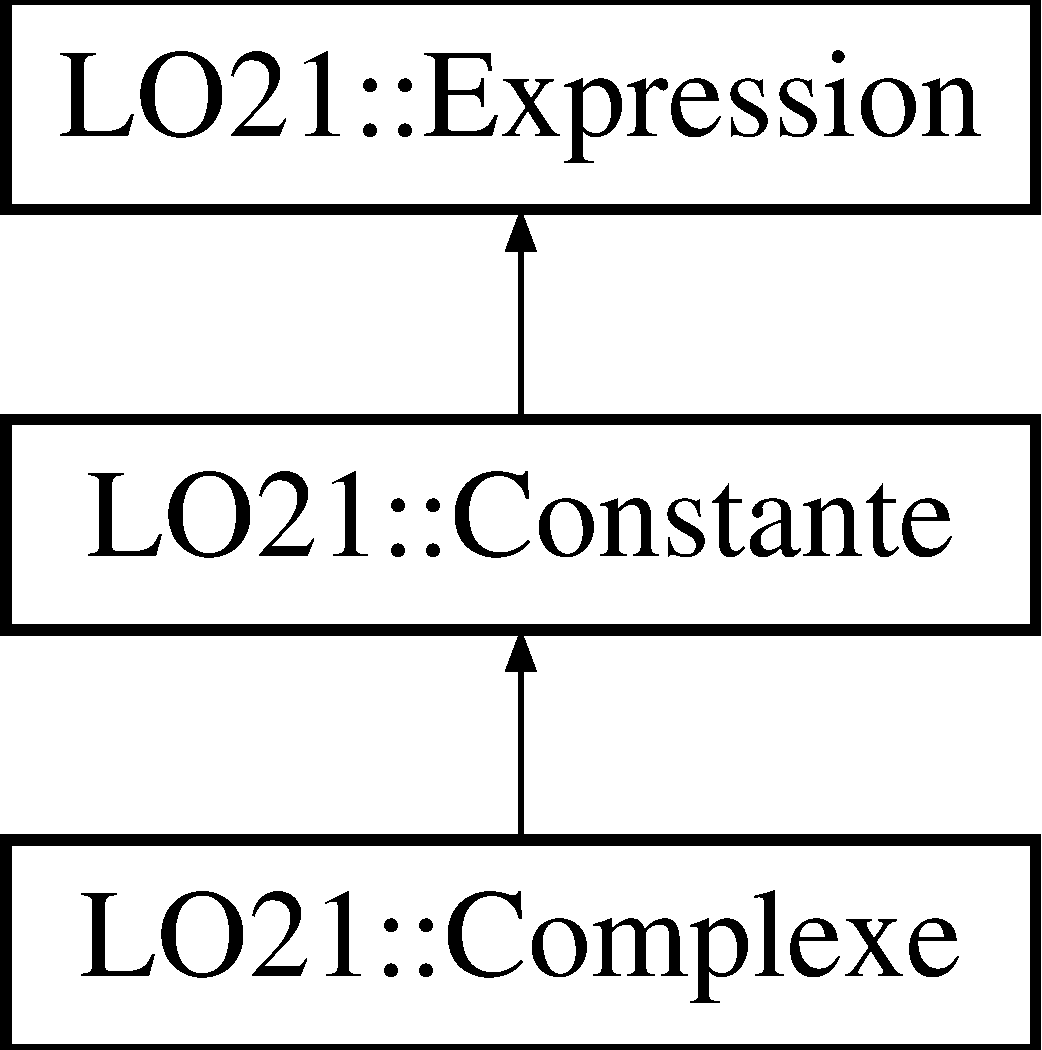
\includegraphics[height=3.000000cm]{class_l_o21_1_1_complexe}
\end{center}
\end{figure}
\subsection*{\-Public \-Member \-Functions}
\begin{DoxyCompactItemize}
\item 
\hypertarget{class_l_o21_1_1_complexe_ae9949fb1e28f1b232c83acafecf67d33}{{\bfseries \-Complexe} (const \hyperlink{class_l_o21_1_1_constante}{\-Constante} \&a, const \hyperlink{class_l_o21_1_1_constante}{\-Constante} \&b)}\label{class_l_o21_1_1_complexe_ae9949fb1e28f1b232c83acafecf67d33}

\item 
\hypertarget{class_l_o21_1_1_complexe_ac92996231047d39d40e11384bb9311b6}{\hyperlink{class_l_o21_1_1_complexe_ac92996231047d39d40e11384bb9311b6}{$\sim$\-Complexe} ()}\label{class_l_o21_1_1_complexe_ac92996231047d39d40e11384bb9311b6}

\begin{DoxyCompactList}\small\item\em \-Destructeur de la classe \hyperlink{class_l_o21_1_1_complexe}{\-Complexe}. \end{DoxyCompactList}\item 
const \hyperlink{class_l_o21_1_1_nombre}{\-Nombre} $\ast$ \hyperlink{class_l_o21_1_1_complexe_a97339c7e868c0b487f69b8b001efed67}{get\-\_\-a} () const 
\begin{DoxyCompactList}\small\item\em \-Retourne la partie reelle du complexe. \end{DoxyCompactList}\item 
const \hyperlink{class_l_o21_1_1_nombre}{\-Nombre} $\ast$ \hyperlink{class_l_o21_1_1_complexe_af2221f90de1c2558ed18020b0f5b10cd}{get\-\_\-b} () const 
\begin{DoxyCompactList}\small\item\em \-Retourne la partie imaginaire du complexe. \end{DoxyCompactList}\item 
\-Q\-String \hyperlink{class_l_o21_1_1_complexe_a327fd83ec9743fb43c5d47831d8ed45c}{to\-String} () const 
\begin{DoxyCompactList}\small\item\em \-Permet l'affichage textuel d'un nombre complexe. \end{DoxyCompactList}\item 
\hyperlink{class_l_o21_1_1_constante}{\-Constante} \& \hyperlink{class_l_o21_1_1_complexe_a6b6c993906543f2fe78d8cb1be6244b3}{module} () const 
\begin{DoxyCompactList}\small\item\em \-Calcule le module d'un complexe. \end{DoxyCompactList}\item 
\hyperlink{class_l_o21_1_1_constante}{\-Constante} \& \hyperlink{class_l_o21_1_1_complexe_ad5808de0a73b0116d8df9ab7d1be599b}{addition} (const \hyperlink{class_l_o21_1_1_constante}{\-Constante} \&nb) const 
\begin{DoxyCompactList}\small\item\em \-Gere l'addition entre un complexe et une constante quelle qu'elle soit. \end{DoxyCompactList}\item 
\hyperlink{class_l_o21_1_1_constante}{\-Constante} \& \hyperlink{class_l_o21_1_1_complexe_a4b699507ed3f22fde85fb4a569fe0f14}{soustraction} (const \hyperlink{class_l_o21_1_1_constante}{\-Constante} \&nb) const 
\begin{DoxyCompactList}\small\item\em \-Gere la soustraction entre un complexe et une constante quelle qu'elle soit. \end{DoxyCompactList}\item 
\hyperlink{class_l_o21_1_1_constante}{\-Constante} \& \hyperlink{class_l_o21_1_1_complexe_aa52efe24813e29d3ae868404c1650cd3}{multiplication} (const \hyperlink{class_l_o21_1_1_constante}{\-Constante} \&nb) const 
\begin{DoxyCompactList}\small\item\em \-Gere la multiplication entre un complexe et une constante quelle qu'elle soit. \end{DoxyCompactList}\item 
\hyperlink{class_l_o21_1_1_constante}{\-Constante} \& \hyperlink{class_l_o21_1_1_complexe_abcf2883f67e57e3ad2b376ea39727fd3}{division} (const \hyperlink{class_l_o21_1_1_constante}{\-Constante} \&nb) const 
\begin{DoxyCompactList}\small\item\em \-Gere la division entre un complexe et une constante quelle qu'elle soit. \end{DoxyCompactList}\item 
\hyperlink{class_l_o21_1_1_constante}{\-Constante} \& \hyperlink{class_l_o21_1_1_complexe_aee563da58f38b8c0295133023f00e09e}{\-S\-I\-G\-N} () const 
\begin{DoxyCompactList}\small\item\em \-Cree un complexe a partir de l'oppose de l'objet appelant. \end{DoxyCompactList}\item 
\hyperlink{class_l_o21_1_1_constante}{\-Constante} \& \hyperlink{class_l_o21_1_1_complexe_a2289c8e181d428d842ed2228f146d1ab}{\-S\-Q\-R} () const 
\begin{DoxyCompactList}\small\item\em \-Effectue le carre d'un nombre complexe. \end{DoxyCompactList}\item 
\hyperlink{class_l_o21_1_1_constante}{\-Constante} \& \hyperlink{class_l_o21_1_1_complexe_af3cba1596766da1820b1e1a52768f145}{\-C\-U\-B\-E} () const 
\begin{DoxyCompactList}\small\item\em \-Effectue le cube d'un nombre complexe. \end{DoxyCompactList}\item 
\hyperlink{class_l_o21_1_1_constante}{\-Constante} \& \hyperlink{class_l_o21_1_1_complexe_a5d383443b7a02ccf583daaadcbff2449}{hook\-Operation} ()
\begin{DoxyCompactList}\small\item\em \-Permet de vérifier le type d'opération et de constante pour instancier correctement un objet. \end{DoxyCompactList}\item 
\hyperlink{class_l_o21_1_1_complexe}{\-Complexe} $\ast$ \hyperlink{class_l_o21_1_1_complexe_a7a7a8d883e959fd7d5f84d5b2b7b2a9e}{clone} () const 
\begin{DoxyCompactList}\small\item\em \-Cree un complexe a partir du complexe appelant. \end{DoxyCompactList}\end{DoxyCompactItemize}


\subsection{\-Detailed \-Description}
\-Classe permettant de gerer les nombres complexes. 

\subsection{\-Member \-Function \-Documentation}
\hypertarget{class_l_o21_1_1_complexe_ad5808de0a73b0116d8df9ab7d1be599b}{\index{\-L\-O21\-::\-Complexe@{\-L\-O21\-::\-Complexe}!addition@{addition}}
\index{addition@{addition}!LO21::Complexe@{\-L\-O21\-::\-Complexe}}
\subsubsection[{addition}]{\setlength{\rightskip}{0pt plus 5cm}{\bf \-Constante} \& {\bf \-Complexe\-::addition} (
\begin{DoxyParamCaption}
\item[{const {\bf \-Constante} \&}]{nb}
\end{DoxyParamCaption}
) const\hspace{0.3cm}{\ttfamily  \mbox{[}virtual\mbox{]}}}}\label{class_l_o21_1_1_complexe_ad5808de0a73b0116d8df9ab7d1be599b}


\-Gere l'addition entre un complexe et une constante quelle qu'elle soit. 

\-Pointeur vers un nombre (\hyperlink{class_l_o21_1_1_entier}{\-Entier}, \hyperlink{class_l_o21_1_1_reel}{\-Reel} ou \hyperlink{class_l_o21_1_1_rationnel}{\-Rationnel}) representant la partie imaginaire du complexe


\begin{DoxyParams}{\-Parameters}
{\em a} & une reference vers une constante (avec verification que celle-\/ci est un nombre et pas un complexe) \\
\hline
{\em b} & une reference vers une constante (avec verification que celle-\/ci est un nombre et pas un complexe)\\
\hline
{\em nb} & une reference vers une constante \\
\hline
\end{DoxyParams}
\begin{DoxyReturn}{\-Returns}
\hyperlink{class_l_o21_1_1_constante}{\-Constante}\& une reference vers la constante creee a partir du resultat 
\end{DoxyReturn}


\-Implements \hyperlink{class_l_o21_1_1_constante_afbe7b10d30d13243c9e6e53c94b9bcb4}{\-L\-O21\-::\-Constante}.

\hypertarget{class_l_o21_1_1_complexe_a7a7a8d883e959fd7d5f84d5b2b7b2a9e}{\index{\-L\-O21\-::\-Complexe@{\-L\-O21\-::\-Complexe}!clone@{clone}}
\index{clone@{clone}!LO21::Complexe@{\-L\-O21\-::\-Complexe}}
\subsubsection[{clone}]{\setlength{\rightskip}{0pt plus 5cm}{\bf \-Complexe} $\ast$ {\bf \-Complexe\-::clone} (
\begin{DoxyParamCaption}
{}
\end{DoxyParamCaption}
) const\hspace{0.3cm}{\ttfamily  \mbox{[}virtual\mbox{]}}}}\label{class_l_o21_1_1_complexe_a7a7a8d883e959fd7d5f84d5b2b7b2a9e}


\-Cree un complexe a partir du complexe appelant. 

\begin{DoxyReturn}{\-Returns}
\-Constante$\ast$ un pointeur vers le complexe cree par recopie 
\end{DoxyReturn}


\-Implements \hyperlink{class_l_o21_1_1_constante_a88ab8ec81b794ed881fba45264133aac}{\-L\-O21\-::\-Constante}.

\hypertarget{class_l_o21_1_1_complexe_af3cba1596766da1820b1e1a52768f145}{\index{\-L\-O21\-::\-Complexe@{\-L\-O21\-::\-Complexe}!\-C\-U\-B\-E@{\-C\-U\-B\-E}}
\index{\-C\-U\-B\-E@{\-C\-U\-B\-E}!LO21::Complexe@{\-L\-O21\-::\-Complexe}}
\subsubsection[{\-C\-U\-B\-E}]{\setlength{\rightskip}{0pt plus 5cm}{\bf \-Constante} \& {\bf \-Complexe\-::\-C\-U\-B\-E} (
\begin{DoxyParamCaption}
{}
\end{DoxyParamCaption}
) const}}\label{class_l_o21_1_1_complexe_af3cba1596766da1820b1e1a52768f145}


\-Effectue le cube d'un nombre complexe. 

\begin{DoxyReturn}{\-Returns}
\hyperlink{class_l_o21_1_1_constante}{\-Constante}\& une reference vers la constante creee a partir du resultat 
\end{DoxyReturn}


\-Reimplemented from \hyperlink{class_l_o21_1_1_constante_a6c1caa0adefa4eaf0429414840542531}{\-L\-O21\-::\-Constante}.

\hypertarget{class_l_o21_1_1_complexe_abcf2883f67e57e3ad2b376ea39727fd3}{\index{\-L\-O21\-::\-Complexe@{\-L\-O21\-::\-Complexe}!division@{division}}
\index{division@{division}!LO21::Complexe@{\-L\-O21\-::\-Complexe}}
\subsubsection[{division}]{\setlength{\rightskip}{0pt plus 5cm}{\bf \-Constante} \& {\bf \-Complexe\-::division} (
\begin{DoxyParamCaption}
\item[{const {\bf \-Constante} \&}]{nb}
\end{DoxyParamCaption}
) const\hspace{0.3cm}{\ttfamily  \mbox{[}virtual\mbox{]}}}}\label{class_l_o21_1_1_complexe_abcf2883f67e57e3ad2b376ea39727fd3}


\-Gere la division entre un complexe et une constante quelle qu'elle soit. 


\begin{DoxyParams}{\-Parameters}
{\em nb} & une reference vers une constante \\
\hline
\end{DoxyParams}
\begin{DoxyReturn}{\-Returns}
\hyperlink{class_l_o21_1_1_constante}{\-Constante}\& une reference vers la constante creee a partir du resultat 
\end{DoxyReturn}


\-Implements \hyperlink{class_l_o21_1_1_constante_a6ffc44753a672f59272792f061c8cd55}{\-L\-O21\-::\-Constante}.

\hypertarget{class_l_o21_1_1_complexe_a97339c7e868c0b487f69b8b001efed67}{\index{\-L\-O21\-::\-Complexe@{\-L\-O21\-::\-Complexe}!get\-\_\-a@{get\-\_\-a}}
\index{get\-\_\-a@{get\-\_\-a}!LO21::Complexe@{\-L\-O21\-::\-Complexe}}
\subsubsection[{get\-\_\-a}]{\setlength{\rightskip}{0pt plus 5cm}const {\bf \-Nombre} $\ast$ {\bf \-Complexe\-::get\-\_\-a} (
\begin{DoxyParamCaption}
{}
\end{DoxyParamCaption}
) const\hspace{0.3cm}{\ttfamily  \mbox{[}inline\mbox{]}}}}\label{class_l_o21_1_1_complexe_a97339c7e868c0b487f69b8b001efed67}


\-Retourne la partie reelle du complexe. 

\begin{DoxyReturn}{\-Returns}
const \-Nombre$\ast$ un pointeur vers le nombre definissant la partie reelle du nombre complexe 
\end{DoxyReturn}
\hypertarget{class_l_o21_1_1_complexe_af2221f90de1c2558ed18020b0f5b10cd}{\index{\-L\-O21\-::\-Complexe@{\-L\-O21\-::\-Complexe}!get\-\_\-b@{get\-\_\-b}}
\index{get\-\_\-b@{get\-\_\-b}!LO21::Complexe@{\-L\-O21\-::\-Complexe}}
\subsubsection[{get\-\_\-b}]{\setlength{\rightskip}{0pt plus 5cm}const {\bf \-Nombre} $\ast$ {\bf \-Complexe\-::get\-\_\-b} (
\begin{DoxyParamCaption}
{}
\end{DoxyParamCaption}
) const\hspace{0.3cm}{\ttfamily  \mbox{[}inline\mbox{]}}}}\label{class_l_o21_1_1_complexe_af2221f90de1c2558ed18020b0f5b10cd}


\-Retourne la partie imaginaire du complexe. 

\begin{DoxyReturn}{\-Returns}
const \-Nombre$\ast$ un pointeur vers le nombre definissant la partie imaginaire du nombre complexe 
\end{DoxyReturn}
\hypertarget{class_l_o21_1_1_complexe_a5d383443b7a02ccf583daaadcbff2449}{\index{\-L\-O21\-::\-Complexe@{\-L\-O21\-::\-Complexe}!hook\-Operation@{hook\-Operation}}
\index{hook\-Operation@{hook\-Operation}!LO21::Complexe@{\-L\-O21\-::\-Complexe}}
\subsubsection[{hook\-Operation}]{\setlength{\rightskip}{0pt plus 5cm}{\bf \-Constante} \& {\bf \-Complexe\-::hook\-Operation} (
\begin{DoxyParamCaption}
{}
\end{DoxyParamCaption}
)\hspace{0.3cm}{\ttfamily  \mbox{[}virtual\mbox{]}}}}\label{class_l_o21_1_1_complexe_a5d383443b7a02ccf583daaadcbff2449}


\-Permet de vérifier le type d'opération et de constante pour instancier correctement un objet. 

\begin{DoxyReturn}{\-Returns}
\hyperlink{class_l_o21_1_1_constante}{\-Constante}\& \-Une reference vers une constante instanciee 
\end{DoxyReturn}


\-Implements \hyperlink{class_l_o21_1_1_constante_a0e0ad1254afea74deb69a05f51220852}{\-L\-O21\-::\-Constante}.

\hypertarget{class_l_o21_1_1_complexe_a6b6c993906543f2fe78d8cb1be6244b3}{\index{\-L\-O21\-::\-Complexe@{\-L\-O21\-::\-Complexe}!module@{module}}
\index{module@{module}!LO21::Complexe@{\-L\-O21\-::\-Complexe}}
\subsubsection[{module}]{\setlength{\rightskip}{0pt plus 5cm}{\bf \-Constante} \& {\bf \-Complexe\-::module} (
\begin{DoxyParamCaption}
{}
\end{DoxyParamCaption}
) const}}\label{class_l_o21_1_1_complexe_a6b6c993906543f2fe78d8cb1be6244b3}


\-Calcule le module d'un complexe. 

\begin{DoxyReturn}{\-Returns}
\hyperlink{class_l_o21_1_1_constante}{\-Constante}\& une reference vers la constante creee a partir du resultat 
\end{DoxyReturn}
\hypertarget{class_l_o21_1_1_complexe_aa52efe24813e29d3ae868404c1650cd3}{\index{\-L\-O21\-::\-Complexe@{\-L\-O21\-::\-Complexe}!multiplication@{multiplication}}
\index{multiplication@{multiplication}!LO21::Complexe@{\-L\-O21\-::\-Complexe}}
\subsubsection[{multiplication}]{\setlength{\rightskip}{0pt plus 5cm}{\bf \-Constante} \& {\bf \-Complexe\-::multiplication} (
\begin{DoxyParamCaption}
\item[{const {\bf \-Constante} \&}]{nb}
\end{DoxyParamCaption}
) const\hspace{0.3cm}{\ttfamily  \mbox{[}virtual\mbox{]}}}}\label{class_l_o21_1_1_complexe_aa52efe24813e29d3ae868404c1650cd3}


\-Gere la multiplication entre un complexe et une constante quelle qu'elle soit. 


\begin{DoxyParams}{\-Parameters}
{\em nb} & une reference vers une constante \\
\hline
\end{DoxyParams}
\begin{DoxyReturn}{\-Returns}
\hyperlink{class_l_o21_1_1_constante}{\-Constante}\& une reference vers la constante creee a partir du resultat 
\end{DoxyReturn}


\-Implements \hyperlink{class_l_o21_1_1_constante_ab2f5d581536b98c0703349fcb6536527}{\-L\-O21\-::\-Constante}.

\hypertarget{class_l_o21_1_1_complexe_aee563da58f38b8c0295133023f00e09e}{\index{\-L\-O21\-::\-Complexe@{\-L\-O21\-::\-Complexe}!\-S\-I\-G\-N@{\-S\-I\-G\-N}}
\index{\-S\-I\-G\-N@{\-S\-I\-G\-N}!LO21::Complexe@{\-L\-O21\-::\-Complexe}}
\subsubsection[{\-S\-I\-G\-N}]{\setlength{\rightskip}{0pt plus 5cm}{\bf \-Constante} \& {\bf \-Complexe\-::\-S\-I\-G\-N} (
\begin{DoxyParamCaption}
{}
\end{DoxyParamCaption}
) const}}\label{class_l_o21_1_1_complexe_aee563da58f38b8c0295133023f00e09e}


\-Cree un complexe a partir de l'oppose de l'objet appelant. 

\begin{DoxyReturn}{\-Returns}
\hyperlink{class_l_o21_1_1_constante}{\-Constante}\& une reference vers la constante creee a partir du resultat 
\end{DoxyReturn}


\-Reimplemented from \hyperlink{class_l_o21_1_1_constante_a279a9cb03a7652957e5f20b2adc1f270}{\-L\-O21\-::\-Constante}.

\hypertarget{class_l_o21_1_1_complexe_a4b699507ed3f22fde85fb4a569fe0f14}{\index{\-L\-O21\-::\-Complexe@{\-L\-O21\-::\-Complexe}!soustraction@{soustraction}}
\index{soustraction@{soustraction}!LO21::Complexe@{\-L\-O21\-::\-Complexe}}
\subsubsection[{soustraction}]{\setlength{\rightskip}{0pt plus 5cm}{\bf \-Constante} \& {\bf \-Complexe\-::soustraction} (
\begin{DoxyParamCaption}
\item[{const {\bf \-Constante} \&}]{nb}
\end{DoxyParamCaption}
) const\hspace{0.3cm}{\ttfamily  \mbox{[}virtual\mbox{]}}}}\label{class_l_o21_1_1_complexe_a4b699507ed3f22fde85fb4a569fe0f14}


\-Gere la soustraction entre un complexe et une constante quelle qu'elle soit. 


\begin{DoxyParams}{\-Parameters}
{\em nb} & une reference vers une constante \\
\hline
\end{DoxyParams}
\begin{DoxyReturn}{\-Returns}
\hyperlink{class_l_o21_1_1_constante}{\-Constante}\& une reference vers la constante creee a partir du resultat 
\end{DoxyReturn}


\-Implements \hyperlink{class_l_o21_1_1_constante_aedf16155a16ea835c61e55c57643fa49}{\-L\-O21\-::\-Constante}.

\hypertarget{class_l_o21_1_1_complexe_a2289c8e181d428d842ed2228f146d1ab}{\index{\-L\-O21\-::\-Complexe@{\-L\-O21\-::\-Complexe}!\-S\-Q\-R@{\-S\-Q\-R}}
\index{\-S\-Q\-R@{\-S\-Q\-R}!LO21::Complexe@{\-L\-O21\-::\-Complexe}}
\subsubsection[{\-S\-Q\-R}]{\setlength{\rightskip}{0pt plus 5cm}{\bf \-Constante} \& {\bf \-Complexe\-::\-S\-Q\-R} (
\begin{DoxyParamCaption}
{}
\end{DoxyParamCaption}
) const}}\label{class_l_o21_1_1_complexe_a2289c8e181d428d842ed2228f146d1ab}


\-Effectue le carre d'un nombre complexe. 

\begin{DoxyReturn}{\-Returns}
\hyperlink{class_l_o21_1_1_constante}{\-Constante}\& une reference vers la constante creee a partir du resultat 
\end{DoxyReturn}


\-Reimplemented from \hyperlink{class_l_o21_1_1_constante_ab3581cf3213fb36e1c19d33e22f1e829}{\-L\-O21\-::\-Constante}.

\hypertarget{class_l_o21_1_1_complexe_a327fd83ec9743fb43c5d47831d8ed45c}{\index{\-L\-O21\-::\-Complexe@{\-L\-O21\-::\-Complexe}!to\-String@{to\-String}}
\index{to\-String@{to\-String}!LO21::Complexe@{\-L\-O21\-::\-Complexe}}
\subsubsection[{to\-String}]{\setlength{\rightskip}{0pt plus 5cm}\-Q\-String {\bf \-Complexe\-::to\-String} (
\begin{DoxyParamCaption}
{}
\end{DoxyParamCaption}
) const\hspace{0.3cm}{\ttfamily  \mbox{[}inline, virtual\mbox{]}}}}\label{class_l_o21_1_1_complexe_a327fd83ec9743fb43c5d47831d8ed45c}


\-Permet l'affichage textuel d'un nombre complexe. 

\begin{DoxyReturn}{\-Returns}
\-Q\-String contenant le texte representant le complexe 
\end{DoxyReturn}


\-Implements \hyperlink{class_l_o21_1_1_expression}{\-L\-O21\-::\-Expression}.



\-The documentation for this class was generated from the following files\-:\begin{DoxyCompactItemize}
\item 
\hyperlink{_complexe_8h}{\-Complexe.\-h}\item 
\-Complexe.\-cpp\end{DoxyCompactItemize}

\hypertarget{class_complexe}{\section{\-Complexe \-Class \-Reference}
\label{class_complexe}\index{\-Complexe@{\-Complexe}}
}


\-Classe permettant de gerer les nombres complexes.  




{\ttfamily \#include $<$\-Option.\-h$>$}



\subsection{\-Detailed \-Description}
\-Classe permettant de gerer les nombres complexes. 

\-The documentation for this class was generated from the following file\-:\begin{DoxyCompactItemize}
\item 
\hyperlink{_option_8h}{\-Option.\-h}\end{DoxyCompactItemize}

\hypertarget{class_l_o21_1_1_constante}{\section{\-L\-O21\-:\-:\-Constante \-Class \-Reference}
\label{class_l_o21_1_1_constante}\index{\-L\-O21\-::\-Constante@{\-L\-O21\-::\-Constante}}
}


\-Definit d'une maniere generale les operations possibles sur les constantes qu'elles soient entieres, reelles, rationnelles ou complexes.  




{\ttfamily \#include $<$\-Constante.\-h$>$}

\-Inheritance diagram for \-L\-O21\-:\-:\-Constante\-:\begin{figure}[H]
\begin{center}
\leavevmode
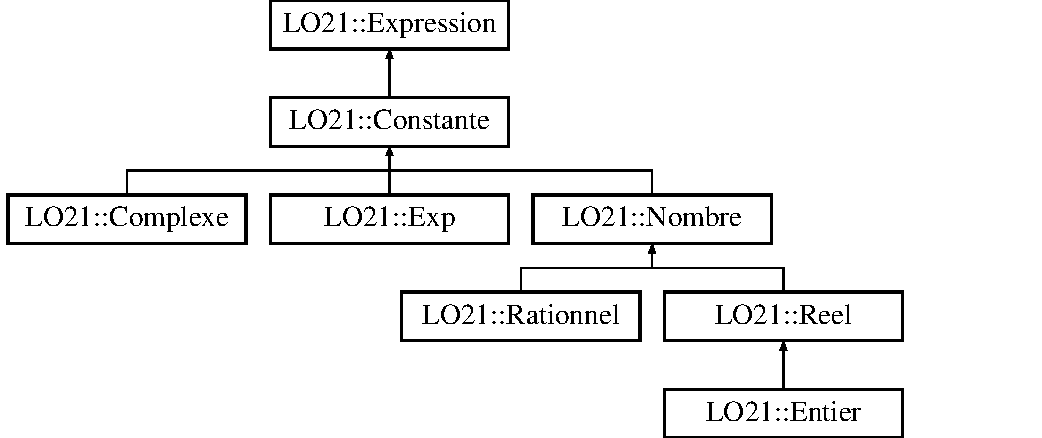
\includegraphics[height=5.000000cm]{class_l_o21_1_1_constante}
\end{center}
\end{figure}
\subsection*{\-Public \-Member \-Functions}
\begin{DoxyCompactItemize}
\item 
\hyperlink{class_l_o21_1_1_constante}{\-Constante} \& \hyperlink{class_l_o21_1_1_constante_a279a9cb03a7652957e5f20b2adc1f270}{\-S\-I\-G\-N} () const 
\begin{DoxyCompactList}\small\item\em \-Retourne l'oppose de la constante. \end{DoxyCompactList}\item 
\hyperlink{class_l_o21_1_1_constante}{\-Constante} \& \hyperlink{class_l_o21_1_1_constante_ab3581cf3213fb36e1c19d33e22f1e829}{\-S\-Q\-R} () const 
\begin{DoxyCompactList}\small\item\em \-Effectue le carre de la constante. \end{DoxyCompactList}\item 
\hyperlink{class_l_o21_1_1_constante}{\-Constante} \& \hyperlink{class_l_o21_1_1_constante_a6c1caa0adefa4eaf0429414840542531}{\-C\-U\-B\-E} () const 
\begin{DoxyCompactList}\small\item\em \-Effectue le cube de la constante. \end{DoxyCompactList}\item 
\hyperlink{class_l_o21_1_1_constante}{\-Constante} \& \hyperlink{class_l_o21_1_1_constante_a3e6291c03f657aa368671857b3ea9440}{operator+} (const \hyperlink{class_l_o21_1_1_constante}{\-Constante} \&nb)
\begin{DoxyCompactList}\small\item\em \-Surcharge de l'operateur + entre deux constantes. \end{DoxyCompactList}\item 
\hyperlink{class_l_o21_1_1_constante}{\-Constante} \& \hyperlink{class_l_o21_1_1_constante_a6e9af4e1804e4ef41bec14f155c83ff5}{operator-\/} (const \hyperlink{class_l_o21_1_1_constante}{\-Constante} \&nb)
\begin{DoxyCompactList}\small\item\em \-Surcharge de l'operateur -\/ entre deux constantes. \end{DoxyCompactList}\item 
\hyperlink{class_l_o21_1_1_constante}{\-Constante} \& \hyperlink{class_l_o21_1_1_constante_ae88587bdfaebe7beb505cea25df2655b}{operator$\ast$} (const \hyperlink{class_l_o21_1_1_constante}{\-Constante} \&nb)
\begin{DoxyCompactList}\small\item\em \-Surcharge de l'operateur $\ast$ entre deux constantes. \end{DoxyCompactList}\item 
\hyperlink{class_l_o21_1_1_constante}{\-Constante} \& \hyperlink{class_l_o21_1_1_constante_ab64f390bb6e24b854cb357fd2dc06a89}{operator/} (const \hyperlink{class_l_o21_1_1_constante}{\-Constante} \&nb)
\begin{DoxyCompactList}\small\item\em \-Surcharge de l'operateur / entre deux constantes. \end{DoxyCompactList}\item 
\hyperlink{classvirtual}{virtual} \hyperlink{class_l_o21_1_1_constante}{\-Constante} \& \hyperlink{class_l_o21_1_1_constante_afbe7b10d30d13243c9e6e53c94b9bcb4}{addition} (const \hyperlink{class_l_o21_1_1_constante}{\-Constante} \&nb) const =0
\begin{DoxyCompactList}\small\item\em \-Gere l'addition entre deux constantes quelles qu'elles soient. \end{DoxyCompactList}\item 
\hyperlink{classvirtual}{virtual} \hyperlink{class_l_o21_1_1_constante}{\-Constante} \& \hyperlink{class_l_o21_1_1_constante_aedf16155a16ea835c61e55c57643fa49}{soustraction} (const \hyperlink{class_l_o21_1_1_constante}{\-Constante} \&nb) const =0
\begin{DoxyCompactList}\small\item\em \-Gere la soustraction entre deux constantes quelles qu'elles soient. \end{DoxyCompactList}\item 
\hyperlink{classvirtual}{virtual} \hyperlink{class_l_o21_1_1_constante}{\-Constante} \& \hyperlink{class_l_o21_1_1_constante_ab2f5d581536b98c0703349fcb6536527}{multiplication} (const \hyperlink{class_l_o21_1_1_constante}{\-Constante} \&nb) const =0
\begin{DoxyCompactList}\small\item\em \-Gere la multiplication entre deux constantes quelles qu'elles soient. \end{DoxyCompactList}\item 
\hyperlink{classvirtual}{virtual} \hyperlink{class_l_o21_1_1_constante}{\-Constante} \& \hyperlink{class_l_o21_1_1_constante_a6ffc44753a672f59272792f061c8cd55}{division} (const \hyperlink{class_l_o21_1_1_constante}{\-Constante} \&nb) const =0
\begin{DoxyCompactList}\small\item\em \-Gere la division entre deux constantes quelles qu'elles soient. \end{DoxyCompactList}\item 
\hyperlink{classvirtual}{virtual} \hyperlink{class_l_o21_1_1_constante}{\-Constante} \& \hyperlink{class_l_o21_1_1_constante_a0e0ad1254afea74deb69a05f51220852}{hook\-Operation} ()=0
\item 
\hypertarget{class_l_o21_1_1_constante_af6774f6830ad656777082e1f3c7e4164}{void \hyperlink{class_l_o21_1_1_constante_af6774f6830ad656777082e1f3c7e4164}{\-E\-V\-A\-L} ()}\label{class_l_o21_1_1_constante_af6774f6830ad656777082e1f3c7e4164}

\begin{DoxyCompactList}\small\item\em \-Evalue une constante. \end{DoxyCompactList}\item 
\hyperlink{class_l_o21_1_1_constante}{\-Constante} $\ast$ \hyperlink{class_l_o21_1_1_constante_a88ab8ec81b794ed881fba45264133aac}{clone} () const =0
\begin{DoxyCompactList}\small\item\em \-Recopie la constante appelante. \end{DoxyCompactList}\end{DoxyCompactItemize}


\subsection{\-Detailed \-Description}
\-Definit d'une maniere generale les operations possibles sur les constantes qu'elles soient entieres, reelles, rationnelles ou complexes. 

\subsection{\-Member \-Function \-Documentation}
\hypertarget{class_l_o21_1_1_constante_afbe7b10d30d13243c9e6e53c94b9bcb4}{\index{\-L\-O21\-::\-Constante@{\-L\-O21\-::\-Constante}!addition@{addition}}
\index{addition@{addition}!LO21::Constante@{\-L\-O21\-::\-Constante}}
\subsubsection[{addition}]{\setlength{\rightskip}{0pt plus 5cm}{\bf \-Constante} \& {\bf \-L\-O21\-::\-Constante\-::addition} (
\begin{DoxyParamCaption}
\item[{const {\bf \-Constante} \&}]{nb}
\end{DoxyParamCaption}
) const\hspace{0.3cm}{\ttfamily  \mbox{[}pure virtual\mbox{]}}}}\label{class_l_o21_1_1_constante_afbe7b10d30d13243c9e6e53c94b9bcb4}


\-Gere l'addition entre deux constantes quelles qu'elles soient. 


\begin{DoxyParams}{\-Parameters}
{\em nb} & une reference vers une constante \\
\hline
\end{DoxyParams}
\begin{DoxyReturn}{\-Returns}
\hyperlink{class_l_o21_1_1_constante}{\-Constante}\& une reference vers la constante creee a partir du resultat 
\end{DoxyReturn}


\-Implemented in \hyperlink{class_l_o21_1_1_nombre_a75c7a5c063ed122f7ba004e09f1f6621}{\-L\-O21\-::\-Nombre}, \hyperlink{class_l_o21_1_1_complexe_ad5808de0a73b0116d8df9ab7d1be599b}{\-L\-O21\-::\-Complexe}, \hyperlink{class_l_o21_1_1_reel_ada705f00ece11942f330bad8497c2cb5}{\-L\-O21\-::\-Reel}, \hyperlink{class_l_o21_1_1_exp_afdb7c0687e2b8cda07ff85bd86299866}{\-L\-O21\-::\-Exp}, \hyperlink{class_l_o21_1_1_entier_a8c70a23f95a29034d78fc5b8c76c4265}{\-L\-O21\-::\-Entier}, and \hyperlink{class_l_o21_1_1_rationnel_a67e3dea6269482abdf3101e16e53c769}{\-L\-O21\-::\-Rationnel}.

\hypertarget{class_l_o21_1_1_constante_a88ab8ec81b794ed881fba45264133aac}{\index{\-L\-O21\-::\-Constante@{\-L\-O21\-::\-Constante}!clone@{clone}}
\index{clone@{clone}!LO21::Constante@{\-L\-O21\-::\-Constante}}
\subsubsection[{clone}]{\setlength{\rightskip}{0pt plus 5cm}{\bf \-Constante} $\ast$ {\bf \-L\-O21\-::\-Constante\-::clone} (
\begin{DoxyParamCaption}
{}
\end{DoxyParamCaption}
) const\hspace{0.3cm}{\ttfamily  \mbox{[}pure virtual\mbox{]}}}}\label{class_l_o21_1_1_constante_a88ab8ec81b794ed881fba45264133aac}


\-Recopie la constante appelante. 

\begin{DoxyReturn}{\-Returns}
\-Constante$\ast$ un pointeur vers la constante creee par recopie 
\end{DoxyReturn}


\-Implements \hyperlink{class_l_o21_1_1_expression_ad2c9e5301c976f9a2d40edaff0332715}{\-L\-O21\-::\-Expression}.



\-Implemented in \hyperlink{class_l_o21_1_1_nombre_aea071e3bcebfdc9337eaea8515e248c9}{\-L\-O21\-::\-Nombre}, \hyperlink{class_l_o21_1_1_complexe_a7a7a8d883e959fd7d5f84d5b2b7b2a9e}{\-L\-O21\-::\-Complexe}, \hyperlink{class_l_o21_1_1_rationnel_aab7de5f24ff5fa9f5d250e8b096ceb34}{\-L\-O21\-::\-Rationnel}, \hyperlink{class_l_o21_1_1_entier_a76f8af45d660b33c6e082986be0a9223}{\-L\-O21\-::\-Entier}, \hyperlink{class_l_o21_1_1_reel_a03bf8d59ba75b2fc45d3db330210201a}{\-L\-O21\-::\-Reel}, and \hyperlink{class_l_o21_1_1_exp_ac6109efb09b218264b5a44db300bfa12}{\-L\-O21\-::\-Exp}.

\hypertarget{class_l_o21_1_1_constante_a6c1caa0adefa4eaf0429414840542531}{\index{\-L\-O21\-::\-Constante@{\-L\-O21\-::\-Constante}!\-C\-U\-B\-E@{\-C\-U\-B\-E}}
\index{\-C\-U\-B\-E@{\-C\-U\-B\-E}!LO21::Constante@{\-L\-O21\-::\-Constante}}
\subsubsection[{\-C\-U\-B\-E}]{\setlength{\rightskip}{0pt plus 5cm}{\bf \-Constante} \& {\bf \-L\-O21\-::\-Constante\-::\-C\-U\-B\-E} (
\begin{DoxyParamCaption}
{}
\end{DoxyParamCaption}
) const}}\label{class_l_o21_1_1_constante_a6c1caa0adefa4eaf0429414840542531}


\-Effectue le cube de la constante. 

\begin{DoxyReturn}{\-Returns}
\hyperlink{class_l_o21_1_1_constante}{\-Constante}\& une reference vers la constante creee a partir du resultat 
\end{DoxyReturn}


\-Reimplemented in \hyperlink{class_l_o21_1_1_complexe_af3cba1596766da1820b1e1a52768f145}{\-L\-O21\-::\-Complexe}.

\hypertarget{class_l_o21_1_1_constante_a6ffc44753a672f59272792f061c8cd55}{\index{\-L\-O21\-::\-Constante@{\-L\-O21\-::\-Constante}!division@{division}}
\index{division@{division}!LO21::Constante@{\-L\-O21\-::\-Constante}}
\subsubsection[{division}]{\setlength{\rightskip}{0pt plus 5cm}{\bf \-Constante} \& {\bf \-L\-O21\-::\-Constante\-::division} (
\begin{DoxyParamCaption}
\item[{const {\bf \-Constante} \&}]{nb}
\end{DoxyParamCaption}
) const\hspace{0.3cm}{\ttfamily  \mbox{[}pure virtual\mbox{]}}}}\label{class_l_o21_1_1_constante_a6ffc44753a672f59272792f061c8cd55}


\-Gere la division entre deux constantes quelles qu'elles soient. 


\begin{DoxyParams}{\-Parameters}
{\em nb} & une reference vers une constante \\
\hline
\end{DoxyParams}
\begin{DoxyReturn}{\-Returns}
\hyperlink{class_l_o21_1_1_constante}{\-Constante}\& une reference vers la constante creee a partir du resultat 
\end{DoxyReturn}


\-Implemented in \hyperlink{class_l_o21_1_1_nombre_aafde3453c22512a8ca152f4013d0f08f}{\-L\-O21\-::\-Nombre}, \hyperlink{class_l_o21_1_1_complexe_abcf2883f67e57e3ad2b376ea39727fd3}{\-L\-O21\-::\-Complexe}, \hyperlink{class_l_o21_1_1_reel_a2b4c6ae1d997ddd4e32e10e4511cfae0}{\-L\-O21\-::\-Reel}, \hyperlink{class_l_o21_1_1_exp_ac957713a5ae0c400745b3c76a5a00eba}{\-L\-O21\-::\-Exp}, \hyperlink{class_l_o21_1_1_entier_a4a9e09753bde4c527596c9a2cda8c87e}{\-L\-O21\-::\-Entier}, and \hyperlink{class_l_o21_1_1_rationnel_abc26382a7434c12b941e8c68547985c4}{\-L\-O21\-::\-Rationnel}.

\hypertarget{class_l_o21_1_1_constante_a0e0ad1254afea74deb69a05f51220852}{\index{\-L\-O21\-::\-Constante@{\-L\-O21\-::\-Constante}!hook\-Operation@{hook\-Operation}}
\index{hook\-Operation@{hook\-Operation}!LO21::Constante@{\-L\-O21\-::\-Constante}}
\subsubsection[{hook\-Operation}]{\setlength{\rightskip}{0pt plus 5cm}{\bf \-Constante} \& {\bf \-L\-O21\-::\-Constante\-::hook\-Operation} (
\begin{DoxyParamCaption}
{}
\end{DoxyParamCaption}
)\hspace{0.3cm}{\ttfamily  \mbox{[}pure virtual\mbox{]}}}}\label{class_l_o21_1_1_constante_a0e0ad1254afea74deb69a05f51220852}
\begin{DoxyReturn}{\-Returns}
\hyperlink{class_l_o21_1_1_constante}{\-Constante}\& \-Une reference vers une constante instanciee 
\end{DoxyReturn}


\-Implemented in \hyperlink{class_l_o21_1_1_nombre_a27247b37ee0159071efbd64bc73d852c}{\-L\-O21\-::\-Nombre}, \hyperlink{class_l_o21_1_1_complexe_a5d383443b7a02ccf583daaadcbff2449}{\-L\-O21\-::\-Complexe}, and \hyperlink{class_l_o21_1_1_exp_a7733be371723e1e003b0ebf713f72124}{\-L\-O21\-::\-Exp}.

\hypertarget{class_l_o21_1_1_constante_ab2f5d581536b98c0703349fcb6536527}{\index{\-L\-O21\-::\-Constante@{\-L\-O21\-::\-Constante}!multiplication@{multiplication}}
\index{multiplication@{multiplication}!LO21::Constante@{\-L\-O21\-::\-Constante}}
\subsubsection[{multiplication}]{\setlength{\rightskip}{0pt plus 5cm}{\bf \-Constante} \& {\bf \-L\-O21\-::\-Constante\-::multiplication} (
\begin{DoxyParamCaption}
\item[{const {\bf \-Constante} \&}]{nb}
\end{DoxyParamCaption}
) const\hspace{0.3cm}{\ttfamily  \mbox{[}pure virtual\mbox{]}}}}\label{class_l_o21_1_1_constante_ab2f5d581536b98c0703349fcb6536527}


\-Gere la multiplication entre deux constantes quelles qu'elles soient. 


\begin{DoxyParams}{\-Parameters}
{\em nb} & une reference vers une constante \\
\hline
\end{DoxyParams}
\begin{DoxyReturn}{\-Returns}
\hyperlink{class_l_o21_1_1_constante}{\-Constante}\& une reference vers la constante creee a partir du resultat 
\end{DoxyReturn}


\-Implemented in \hyperlink{class_l_o21_1_1_nombre_a63cf8dbd304585fe106e8eeebe8c4e89}{\-L\-O21\-::\-Nombre}, \hyperlink{class_l_o21_1_1_complexe_aa52efe24813e29d3ae868404c1650cd3}{\-L\-O21\-::\-Complexe}, \hyperlink{class_l_o21_1_1_reel_a01e5dc973684a30f98f7bde0d0c5840d}{\-L\-O21\-::\-Reel}, \hyperlink{class_l_o21_1_1_exp_a6f72d9ff76fa8479d8e035eb4d1f30f0}{\-L\-O21\-::\-Exp}, \hyperlink{class_l_o21_1_1_entier_a34fdbc8acc0a18318916312983dc78f9}{\-L\-O21\-::\-Entier}, and \hyperlink{class_l_o21_1_1_rationnel_ad59a24eab43b40d59e639078a9a9d638}{\-L\-O21\-::\-Rationnel}.

\hypertarget{class_l_o21_1_1_constante_ae88587bdfaebe7beb505cea25df2655b}{\index{\-L\-O21\-::\-Constante@{\-L\-O21\-::\-Constante}!operator$\ast$@{operator$\ast$}}
\index{operator$\ast$@{operator$\ast$}!LO21::Constante@{\-L\-O21\-::\-Constante}}
\subsubsection[{operator$\ast$}]{\setlength{\rightskip}{0pt plus 5cm}{\bf \-Constante} \& \-L\-O21\-::\-Constante\-::operator$\ast$ (
\begin{DoxyParamCaption}
\item[{const {\bf \-Constante} \&}]{nb}
\end{DoxyParamCaption}
)\hspace{0.3cm}{\ttfamily  \mbox{[}inline\mbox{]}}}}\label{class_l_o21_1_1_constante_ae88587bdfaebe7beb505cea25df2655b}


\-Surcharge de l'operateur $\ast$ entre deux constantes. 


\begin{DoxyParams}{\-Parameters}
{\em nb} & une reference vers une constante \\
\hline
\end{DoxyParams}
\begin{DoxyReturn}{\-Returns}
\hyperlink{class_l_o21_1_1_constante}{\-Constante}\& une reference vers la constante creee a partir du resultat 
\end{DoxyReturn}
\hypertarget{class_l_o21_1_1_constante_a3e6291c03f657aa368671857b3ea9440}{\index{\-L\-O21\-::\-Constante@{\-L\-O21\-::\-Constante}!operator+@{operator+}}
\index{operator+@{operator+}!LO21::Constante@{\-L\-O21\-::\-Constante}}
\subsubsection[{operator+}]{\setlength{\rightskip}{0pt plus 5cm}{\bf \-Constante} \& \-L\-O21\-::\-Constante\-::operator+ (
\begin{DoxyParamCaption}
\item[{const {\bf \-Constante} \&}]{nb}
\end{DoxyParamCaption}
)\hspace{0.3cm}{\ttfamily  \mbox{[}inline\mbox{]}}}}\label{class_l_o21_1_1_constante_a3e6291c03f657aa368671857b3ea9440}


\-Surcharge de l'operateur + entre deux constantes. 


\begin{DoxyParams}{\-Parameters}
{\em nb} & une reference vers une constante \\
\hline
\end{DoxyParams}
\begin{DoxyReturn}{\-Returns}
\hyperlink{class_l_o21_1_1_constante}{\-Constante}\& une reference vers la constante creee a partir du resultat 
\end{DoxyReturn}
\hypertarget{class_l_o21_1_1_constante_a6e9af4e1804e4ef41bec14f155c83ff5}{\index{\-L\-O21\-::\-Constante@{\-L\-O21\-::\-Constante}!operator-\/@{operator-\/}}
\index{operator-\/@{operator-\/}!LO21::Constante@{\-L\-O21\-::\-Constante}}
\subsubsection[{operator-\/}]{\setlength{\rightskip}{0pt plus 5cm}{\bf \-Constante} \& \-L\-O21\-::\-Constante\-::operator-\/ (
\begin{DoxyParamCaption}
\item[{const {\bf \-Constante} \&}]{nb}
\end{DoxyParamCaption}
)\hspace{0.3cm}{\ttfamily  \mbox{[}inline\mbox{]}}}}\label{class_l_o21_1_1_constante_a6e9af4e1804e4ef41bec14f155c83ff5}


\-Surcharge de l'operateur -\/ entre deux constantes. 


\begin{DoxyParams}{\-Parameters}
{\em nb} & une reference vers une constante \\
\hline
\end{DoxyParams}
\begin{DoxyReturn}{\-Returns}
\hyperlink{class_l_o21_1_1_constante}{\-Constante}\& une reference vers la constante creee a partir du resultat 
\end{DoxyReturn}
\hypertarget{class_l_o21_1_1_constante_ab64f390bb6e24b854cb357fd2dc06a89}{\index{\-L\-O21\-::\-Constante@{\-L\-O21\-::\-Constante}!operator/@{operator/}}
\index{operator/@{operator/}!LO21::Constante@{\-L\-O21\-::\-Constante}}
\subsubsection[{operator/}]{\setlength{\rightskip}{0pt plus 5cm}{\bf \-Constante} \& \-L\-O21\-::\-Constante\-::operator/ (
\begin{DoxyParamCaption}
\item[{const {\bf \-Constante} \&}]{nb}
\end{DoxyParamCaption}
)\hspace{0.3cm}{\ttfamily  \mbox{[}inline\mbox{]}}}}\label{class_l_o21_1_1_constante_ab64f390bb6e24b854cb357fd2dc06a89}


\-Surcharge de l'operateur / entre deux constantes. 


\begin{DoxyParams}{\-Parameters}
{\em nb} & une reference vers une constante \\
\hline
\end{DoxyParams}
\begin{DoxyReturn}{\-Returns}
\hyperlink{class_l_o21_1_1_constante}{\-Constante}\& une reference vers la constante creee a partir du resultat 
\end{DoxyReturn}
\hypertarget{class_l_o21_1_1_constante_a279a9cb03a7652957e5f20b2adc1f270}{\index{\-L\-O21\-::\-Constante@{\-L\-O21\-::\-Constante}!\-S\-I\-G\-N@{\-S\-I\-G\-N}}
\index{\-S\-I\-G\-N@{\-S\-I\-G\-N}!LO21::Constante@{\-L\-O21\-::\-Constante}}
\subsubsection[{\-S\-I\-G\-N}]{\setlength{\rightskip}{0pt plus 5cm}{\bf \-Constante} \& {\bf \-L\-O21\-::\-Constante\-::\-S\-I\-G\-N} (
\begin{DoxyParamCaption}
{}
\end{DoxyParamCaption}
) const}}\label{class_l_o21_1_1_constante_a279a9cb03a7652957e5f20b2adc1f270}


\-Retourne l'oppose de la constante. 

\begin{DoxyReturn}{\-Returns}
\hyperlink{class_l_o21_1_1_constante}{\-Constante}\& une reference vers la constante creee a partir du resultat 
\end{DoxyReturn}


\-Reimplemented in \hyperlink{class_l_o21_1_1_nombre_ac420c18d67faf83c1e0751be1c69579d}{\-L\-O21\-::\-Nombre}, and \hyperlink{class_l_o21_1_1_complexe_aee563da58f38b8c0295133023f00e09e}{\-L\-O21\-::\-Complexe}.

\hypertarget{class_l_o21_1_1_constante_aedf16155a16ea835c61e55c57643fa49}{\index{\-L\-O21\-::\-Constante@{\-L\-O21\-::\-Constante}!soustraction@{soustraction}}
\index{soustraction@{soustraction}!LO21::Constante@{\-L\-O21\-::\-Constante}}
\subsubsection[{soustraction}]{\setlength{\rightskip}{0pt plus 5cm}{\bf \-Constante} \& {\bf \-L\-O21\-::\-Constante\-::soustraction} (
\begin{DoxyParamCaption}
\item[{const {\bf \-Constante} \&}]{nb}
\end{DoxyParamCaption}
) const\hspace{0.3cm}{\ttfamily  \mbox{[}pure virtual\mbox{]}}}}\label{class_l_o21_1_1_constante_aedf16155a16ea835c61e55c57643fa49}


\-Gere la soustraction entre deux constantes quelles qu'elles soient. 


\begin{DoxyParams}{\-Parameters}
{\em nb} & une reference vers une constante \\
\hline
\end{DoxyParams}
\begin{DoxyReturn}{\-Returns}
\hyperlink{class_l_o21_1_1_constante}{\-Constante}\& une reference vers la constante creee a partir du resultat 
\end{DoxyReturn}


\-Implemented in \hyperlink{class_l_o21_1_1_nombre_a1e412b0e89c0b68c0ee04a3078c098b1}{\-L\-O21\-::\-Nombre}, \hyperlink{class_l_o21_1_1_complexe_a4b699507ed3f22fde85fb4a569fe0f14}{\-L\-O21\-::\-Complexe}, \hyperlink{class_l_o21_1_1_reel_a9e9ed5805f01d5661aa26c5f626e10ad}{\-L\-O21\-::\-Reel}, \hyperlink{class_l_o21_1_1_exp_ab4f295f8ce2768312576d76c26b6caa7}{\-L\-O21\-::\-Exp}, \hyperlink{class_l_o21_1_1_entier_aa9ebbf0b51016b7e14a12909ed6ab7bb}{\-L\-O21\-::\-Entier}, and \hyperlink{class_l_o21_1_1_rationnel_a3e0d87746663be866be81543d552b6a1}{\-L\-O21\-::\-Rationnel}.

\hypertarget{class_l_o21_1_1_constante_ab3581cf3213fb36e1c19d33e22f1e829}{\index{\-L\-O21\-::\-Constante@{\-L\-O21\-::\-Constante}!\-S\-Q\-R@{\-S\-Q\-R}}
\index{\-S\-Q\-R@{\-S\-Q\-R}!LO21::Constante@{\-L\-O21\-::\-Constante}}
\subsubsection[{\-S\-Q\-R}]{\setlength{\rightskip}{0pt plus 5cm}{\bf \-Constante} \& {\bf \-L\-O21\-::\-Constante\-::\-S\-Q\-R} (
\begin{DoxyParamCaption}
{}
\end{DoxyParamCaption}
) const}}\label{class_l_o21_1_1_constante_ab3581cf3213fb36e1c19d33e22f1e829}


\-Effectue le carre de la constante. 

\begin{DoxyReturn}{\-Returns}
\hyperlink{class_l_o21_1_1_constante}{\-Constante}\& une reference vers la constante creee a partir du resultat 
\end{DoxyReturn}


\-Reimplemented in \hyperlink{class_l_o21_1_1_complexe_a2289c8e181d428d842ed2228f146d1ab}{\-L\-O21\-::\-Complexe}.



\-The documentation for this class was generated from the following files\-:\begin{DoxyCompactItemize}
\item 
\hyperlink{_constante_8h}{\-Constante.\-h}\item 
\-Constante.\-cpp\end{DoxyCompactItemize}

\hypertarget{class_l_o21_1_1_entier}{\section{\-L\-O21\-:\-:\-Entier \-Class \-Reference}
\label{class_l_o21_1_1_entier}\index{\-L\-O21\-::\-Entier@{\-L\-O21\-::\-Entier}}
}


\-Classe representant un entier \-La classe gere les operations sur les entiers positifs et negatifs.  




{\ttfamily \#include $<$\-Entier.\-h$>$}

\-Inheritance diagram for \-L\-O21\-:\-:\-Entier\-:\begin{figure}[H]
\begin{center}
\leavevmode
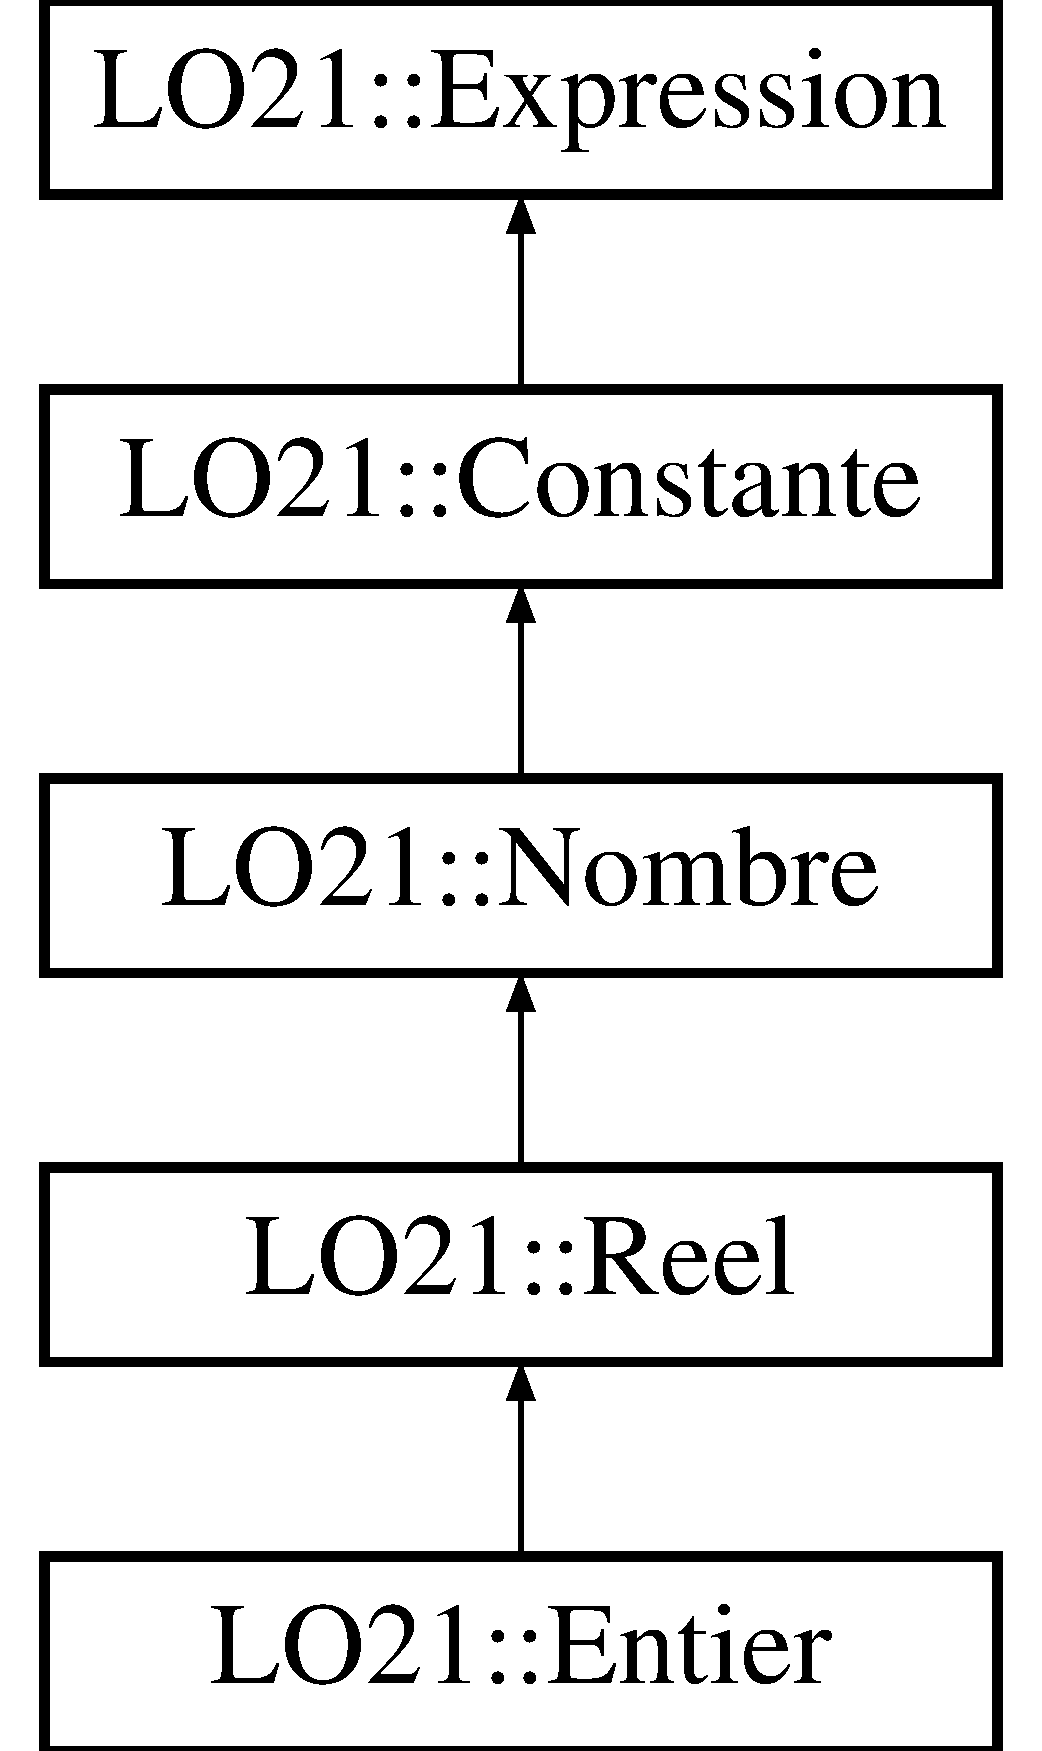
\includegraphics[height=5.000000cm]{class_l_o21_1_1_entier}
\end{center}
\end{figure}
\subsection*{\-Public \-Member \-Functions}
\begin{DoxyCompactItemize}
\item 
\hyperlink{class_l_o21_1_1_constante}{\-Constante} \& \hyperlink{class_l_o21_1_1_entier_a8c70a23f95a29034d78fc5b8c76c4265}{addition} (const \hyperlink{class_l_o21_1_1_constante}{\-Constante} \&nb) const 
\begin{DoxyCompactList}\small\item\em \-Gere l'addition entre un entier et une constante quelle qu'elle soit. \end{DoxyCompactList}\item 
\hyperlink{class_l_o21_1_1_constante}{\-Constante} \& \hyperlink{class_l_o21_1_1_entier_aa9ebbf0b51016b7e14a12909ed6ab7bb}{soustraction} (const \hyperlink{class_l_o21_1_1_constante}{\-Constante} \&nb) const 
\begin{DoxyCompactList}\small\item\em \-Gere la soustraction entre un entier et une constante quelle qu'elle soit. \end{DoxyCompactList}\item 
\hyperlink{class_l_o21_1_1_constante}{\-Constante} \& \hyperlink{class_l_o21_1_1_entier_a34fdbc8acc0a18318916312983dc78f9}{multiplication} (const \hyperlink{class_l_o21_1_1_constante}{\-Constante} \&nb) const 
\begin{DoxyCompactList}\small\item\em \-Gere la multiplication entre un entier et une constante quelle qu'elle soit. \end{DoxyCompactList}\item 
\hyperlink{class_l_o21_1_1_constante}{\-Constante} \& \hyperlink{class_l_o21_1_1_entier_a4a9e09753bde4c527596c9a2cda8c87e}{division} (const \hyperlink{class_l_o21_1_1_constante}{\-Constante} \&nb) const 
\begin{DoxyCompactList}\small\item\em \-Gere la division entre un entier et une constante quelle qu'elle soit. \end{DoxyCompactList}\item 
\-Q\-String \hyperlink{class_l_o21_1_1_entier_a8741d3caf244a1993d478b7353b5a65e}{to\-String} () const 
\begin{DoxyCompactList}\small\item\em \-Permet d'afficher sous forme textuelle un objet \hyperlink{class_l_o21_1_1_entier}{\-Entier}. \end{DoxyCompactList}\item 
\hyperlink{class_l_o21_1_1_rationnel}{\-Rationnel} \& \hyperlink{class_l_o21_1_1_entier_a1039b5ecf2ba82f2f8967d52eb81e2b2}{to\-Rationnel} () const 
\begin{DoxyCompactList}\small\item\em \-Transforme un entier en rationnel. \end{DoxyCompactList}\item 
\hyperlink{class_l_o21_1_1_reel}{\-Reel} \& \hyperlink{class_l_o21_1_1_entier_a1e41e6a2514d7e0b01b8ed6b245fd901}{to\-Reel} () const 
\begin{DoxyCompactList}\small\item\em \-Transforme un entier en reel. \end{DoxyCompactList}\item 
\hyperlink{class_l_o21_1_1_complexe}{\-Complexe} \& \hyperlink{class_l_o21_1_1_entier_abc46eb792359f8dc47785b12837571e3}{to\-Complexe} () const 
\begin{DoxyCompactList}\small\item\em \-Transforme un entier en complexe. \end{DoxyCompactList}\item 
\hyperlink{class_l_o21_1_1_entier}{\-Entier} \& \hyperlink{class_l_o21_1_1_entier_abe27251b6086929c2b2279985e18b752}{\-M\-O\-D} (const \hyperlink{class_l_o21_1_1_entier}{\-Entier} \&nb)
\begin{DoxyCompactList}\small\item\em \-Permet d'appliquer l'operateur modulo sur un entier. \end{DoxyCompactList}\item 
\hyperlink{class_l_o21_1_1_entier}{\-Entier} \& \hyperlink{class_l_o21_1_1_entier_aec2695af3a4a9754ddde3c09a89fda83}{\-F\-A\-C\-T\-O\-R\-I\-E\-L\-L\-E} ()
\begin{DoxyCompactList}\small\item\em \-Permet de calculer la factorielle d'un entier. \end{DoxyCompactList}\item 
int \hyperlink{class_l_o21_1_1_entier_a144f7ad9fd1d1de79503aa647c53d758}{get\-\_\-x} () const 
\begin{DoxyCompactList}\small\item\em \-Retourne l'entier utilise dans l'objet \hyperlink{class_l_o21_1_1_entier}{\-Entier}. \end{DoxyCompactList}\item 
\hyperlink{class_l_o21_1_1_entier_a725b26cfe72bbbbb380a3a6166e7643f}{\-Entier} (int x=0)
\begin{DoxyCompactList}\small\item\em \-Constructeur de la classe \hyperlink{class_l_o21_1_1_entier}{\-Entier}. \end{DoxyCompactList}\item 
bool \hyperlink{class_l_o21_1_1_entier_aefa913cae22177927e3c9d15b00eaac5}{operator==} (const \hyperlink{class_l_o21_1_1_entier}{\-Entier} \&e)
\begin{DoxyCompactList}\small\item\em \-Teste si la valeur d'un \hyperlink{class_l_o21_1_1_entier}{\-Entier} est egale a la valeur d'un autre \hyperlink{class_l_o21_1_1_entier}{\-Entier}. \end{DoxyCompactList}\item 
\hyperlink{class_l_o21_1_1_entier}{\-Entier} $\ast$ \hyperlink{class_l_o21_1_1_entier_a76f8af45d660b33c6e082986be0a9223}{clone} () const 
\begin{DoxyCompactList}\small\item\em \-Recopie l'objet \hyperlink{class_l_o21_1_1_entier}{\-Entier} appelant. \end{DoxyCompactList}\end{DoxyCompactItemize}


\subsection{\-Detailed \-Description}
\-Classe representant un entier \-La classe gere les operations sur les entiers positifs et negatifs. 

\-Calcule le plus grand denominateur commun entre deux entiers.

\hyperlink{class_l_o21_1_1_entier}{\-Entier}\& a, const \hyperlink{class_l_o21_1_1_entier}{\-Entier}\& b) 
\begin{DoxyParams}{\-Parameters}
{\em a} & une reference vers un entier \\
\hline
{\em b} & une reference vers un entier \\
\hline
\end{DoxyParams}
\begin{DoxyReturn}{\-Returns}
\hyperlink{class_l_o21_1_1_entier}{\-Entier} \-Un entier contenant le resultat calcule 
\end{DoxyReturn}


\subsection{\-Constructor \& \-Destructor \-Documentation}
\hypertarget{class_l_o21_1_1_entier_a725b26cfe72bbbbb380a3a6166e7643f}{\index{\-L\-O21\-::\-Entier@{\-L\-O21\-::\-Entier}!\-Entier@{\-Entier}}
\index{\-Entier@{\-Entier}!LO21::Entier@{\-L\-O21\-::\-Entier}}
\subsubsection[{\-Entier}]{\setlength{\rightskip}{0pt plus 5cm}{\bf \-L\-O21\-::\-Entier\-::\-Entier} (
\begin{DoxyParamCaption}
\item[{int}]{x = {\ttfamily 0}}
\end{DoxyParamCaption}
)\hspace{0.3cm}{\ttfamily  \mbox{[}inline\mbox{]}}}}\label{class_l_o21_1_1_entier_a725b26cfe72bbbbb380a3a6166e7643f}


\-Constructeur de la classe \hyperlink{class_l_o21_1_1_entier}{\-Entier}. 


\begin{DoxyParams}{\-Parameters}
{\em x} & l'entier dont on veut la correspondance dans notre classe \hyperlink{class_l_o21_1_1_entier}{\-Entier} \\
\hline
\end{DoxyParams}


\subsection{\-Member \-Function \-Documentation}
\hypertarget{class_l_o21_1_1_entier_a8c70a23f95a29034d78fc5b8c76c4265}{\index{\-L\-O21\-::\-Entier@{\-L\-O21\-::\-Entier}!addition@{addition}}
\index{addition@{addition}!LO21::Entier@{\-L\-O21\-::\-Entier}}
\subsubsection[{addition}]{\setlength{\rightskip}{0pt plus 5cm}{\bf \-Constante} \& {\bf \-L\-O21\-::\-Entier\-::addition} (
\begin{DoxyParamCaption}
\item[{const {\bf \-Constante} \&}]{nb}
\end{DoxyParamCaption}
) const\hspace{0.3cm}{\ttfamily  \mbox{[}virtual\mbox{]}}}}\label{class_l_o21_1_1_entier_a8c70a23f95a29034d78fc5b8c76c4265}


\-Gere l'addition entre un entier et une constante quelle qu'elle soit. 

\-L'entier


\begin{DoxyParams}{\-Parameters}
{\em nb} & une reference vers une constante \\
\hline
\end{DoxyParams}
\begin{DoxyReturn}{\-Returns}
\hyperlink{class_l_o21_1_1_constante}{\-Constante}\& une reference vers la constante creee a partir du resultat 
\end{DoxyReturn}


\-Reimplemented from \hyperlink{class_l_o21_1_1_reel_ada705f00ece11942f330bad8497c2cb5}{\-L\-O21\-::\-Reel}.

\hypertarget{class_l_o21_1_1_entier_a76f8af45d660b33c6e082986be0a9223}{\index{\-L\-O21\-::\-Entier@{\-L\-O21\-::\-Entier}!clone@{clone}}
\index{clone@{clone}!LO21::Entier@{\-L\-O21\-::\-Entier}}
\subsubsection[{clone}]{\setlength{\rightskip}{0pt plus 5cm}{\bf \-Entier} $\ast$ {\bf \-L\-O21\-::\-Entier\-::clone} (
\begin{DoxyParamCaption}
{}
\end{DoxyParamCaption}
) const\hspace{0.3cm}{\ttfamily  \mbox{[}virtual\mbox{]}}}}\label{class_l_o21_1_1_entier_a76f8af45d660b33c6e082986be0a9223}


\-Recopie l'objet \hyperlink{class_l_o21_1_1_entier}{\-Entier} appelant. 

\begin{DoxyReturn}{\-Returns}
\-Entier$\ast$ un pointeur vers l'objet \hyperlink{class_l_o21_1_1_entier}{\-Entier} cree 
\end{DoxyReturn}


\-Reimplemented from \hyperlink{class_l_o21_1_1_reel_a03bf8d59ba75b2fc45d3db330210201a}{\-L\-O21\-::\-Reel}.

\hypertarget{class_l_o21_1_1_entier_a4a9e09753bde4c527596c9a2cda8c87e}{\index{\-L\-O21\-::\-Entier@{\-L\-O21\-::\-Entier}!division@{division}}
\index{division@{division}!LO21::Entier@{\-L\-O21\-::\-Entier}}
\subsubsection[{division}]{\setlength{\rightskip}{0pt plus 5cm}{\bf \-Constante} \& {\bf \-L\-O21\-::\-Entier\-::division} (
\begin{DoxyParamCaption}
\item[{const {\bf \-Constante} \&}]{nb}
\end{DoxyParamCaption}
) const\hspace{0.3cm}{\ttfamily  \mbox{[}virtual\mbox{]}}}}\label{class_l_o21_1_1_entier_a4a9e09753bde4c527596c9a2cda8c87e}


\-Gere la division entre un entier et une constante quelle qu'elle soit. 


\begin{DoxyParams}{\-Parameters}
{\em nb} & une reference vers une constante \\
\hline
\end{DoxyParams}
\begin{DoxyReturn}{\-Returns}
\hyperlink{class_l_o21_1_1_constante}{\-Constante}\& une reference vers la constante creee a partir du resultat 
\end{DoxyReturn}


\-Reimplemented from \hyperlink{class_l_o21_1_1_reel_a2b4c6ae1d997ddd4e32e10e4511cfae0}{\-L\-O21\-::\-Reel}.

\hypertarget{class_l_o21_1_1_entier_aec2695af3a4a9754ddde3c09a89fda83}{\index{\-L\-O21\-::\-Entier@{\-L\-O21\-::\-Entier}!\-F\-A\-C\-T\-O\-R\-I\-E\-L\-L\-E@{\-F\-A\-C\-T\-O\-R\-I\-E\-L\-L\-E}}
\index{\-F\-A\-C\-T\-O\-R\-I\-E\-L\-L\-E@{\-F\-A\-C\-T\-O\-R\-I\-E\-L\-L\-E}!LO21::Entier@{\-L\-O21\-::\-Entier}}
\subsubsection[{\-F\-A\-C\-T\-O\-R\-I\-E\-L\-L\-E}]{\setlength{\rightskip}{0pt plus 5cm}{\bf \-Entier} \& {\bf \-L\-O21\-::\-Entier\-::\-F\-A\-C\-T\-O\-R\-I\-E\-L\-L\-E} (
\begin{DoxyParamCaption}
{}
\end{DoxyParamCaption}
)}}\label{class_l_o21_1_1_entier_aec2695af3a4a9754ddde3c09a89fda83}


\-Permet de calculer la factorielle d'un entier. 

\begin{DoxyReturn}{\-Returns}
\hyperlink{class_l_o21_1_1_entier}{\-Entier}\& une reference vers l'entier cree a partir du resultat 
\end{DoxyReturn}
\hypertarget{class_l_o21_1_1_entier_a144f7ad9fd1d1de79503aa647c53d758}{\index{\-L\-O21\-::\-Entier@{\-L\-O21\-::\-Entier}!get\-\_\-x@{get\-\_\-x}}
\index{get\-\_\-x@{get\-\_\-x}!LO21::Entier@{\-L\-O21\-::\-Entier}}
\subsubsection[{get\-\_\-x}]{\setlength{\rightskip}{0pt plus 5cm}int {\bf \-L\-O21\-::\-Entier\-::get\-\_\-x} (
\begin{DoxyParamCaption}
{}
\end{DoxyParamCaption}
) const\hspace{0.3cm}{\ttfamily  \mbox{[}inline\mbox{]}}}}\label{class_l_o21_1_1_entier_a144f7ad9fd1d1de79503aa647c53d758}


\-Retourne l'entier utilise dans l'objet \hyperlink{class_l_o21_1_1_entier}{\-Entier}. 

\begin{DoxyReturn}{\-Returns}
int l'entier utilise comme attribut de l'objet \hyperlink{class_l_o21_1_1_entier}{\-Entier} 
\end{DoxyReturn}


\-Reimplemented from \hyperlink{class_l_o21_1_1_reel_a2a989b2cac3a15ae99d22f39111f19c6}{\-L\-O21\-::\-Reel}.

\hypertarget{class_l_o21_1_1_entier_abe27251b6086929c2b2279985e18b752}{\index{\-L\-O21\-::\-Entier@{\-L\-O21\-::\-Entier}!\-M\-O\-D@{\-M\-O\-D}}
\index{\-M\-O\-D@{\-M\-O\-D}!LO21::Entier@{\-L\-O21\-::\-Entier}}
\subsubsection[{\-M\-O\-D}]{\setlength{\rightskip}{0pt plus 5cm}{\bf \-Entier} \& {\bf \-L\-O21\-::\-Entier\-::\-M\-O\-D} (
\begin{DoxyParamCaption}
\item[{const {\bf \-Entier} \&}]{nb}
\end{DoxyParamCaption}
)}}\label{class_l_o21_1_1_entier_abe27251b6086929c2b2279985e18b752}


\-Permet d'appliquer l'operateur modulo sur un entier. 


\begin{DoxyParams}{\-Parameters}
{\em nb} & l'entier parametre du modulo \\
\hline
\end{DoxyParams}
\begin{DoxyReturn}{\-Returns}
\hyperlink{class_l_o21_1_1_entier}{\-Entier}\& une reference vers l'entier resultant du modulo 
\end{DoxyReturn}
\hypertarget{class_l_o21_1_1_entier_a34fdbc8acc0a18318916312983dc78f9}{\index{\-L\-O21\-::\-Entier@{\-L\-O21\-::\-Entier}!multiplication@{multiplication}}
\index{multiplication@{multiplication}!LO21::Entier@{\-L\-O21\-::\-Entier}}
\subsubsection[{multiplication}]{\setlength{\rightskip}{0pt plus 5cm}{\bf \-Constante} \& {\bf \-L\-O21\-::\-Entier\-::multiplication} (
\begin{DoxyParamCaption}
\item[{const {\bf \-Constante} \&}]{nb}
\end{DoxyParamCaption}
) const\hspace{0.3cm}{\ttfamily  \mbox{[}virtual\mbox{]}}}}\label{class_l_o21_1_1_entier_a34fdbc8acc0a18318916312983dc78f9}


\-Gere la multiplication entre un entier et une constante quelle qu'elle soit. 


\begin{DoxyParams}{\-Parameters}
{\em nb} & une reference vers une constante \\
\hline
\end{DoxyParams}
\begin{DoxyReturn}{\-Returns}
\hyperlink{class_l_o21_1_1_constante}{\-Constante}\& une reference vers la constante creee a partir du resultat 
\end{DoxyReturn}


\-Reimplemented from \hyperlink{class_l_o21_1_1_reel_a01e5dc973684a30f98f7bde0d0c5840d}{\-L\-O21\-::\-Reel}.

\hypertarget{class_l_o21_1_1_entier_aefa913cae22177927e3c9d15b00eaac5}{\index{\-L\-O21\-::\-Entier@{\-L\-O21\-::\-Entier}!operator==@{operator==}}
\index{operator==@{operator==}!LO21::Entier@{\-L\-O21\-::\-Entier}}
\subsubsection[{operator==}]{\setlength{\rightskip}{0pt plus 5cm}bool \-L\-O21\-::\-Entier\-::operator== (
\begin{DoxyParamCaption}
\item[{const {\bf \-Entier} \&}]{e}
\end{DoxyParamCaption}
)\hspace{0.3cm}{\ttfamily  \mbox{[}inline\mbox{]}}}}\label{class_l_o21_1_1_entier_aefa913cae22177927e3c9d15b00eaac5}


\-Teste si la valeur d'un \hyperlink{class_l_o21_1_1_entier}{\-Entier} est egale a la valeur d'un autre \hyperlink{class_l_o21_1_1_entier}{\-Entier}. 


\begin{DoxyParams}{\-Parameters}
{\em e} & l'\hyperlink{class_l_o21_1_1_entier}{\-Entier} dont la valeur est a tester \\
\hline
\end{DoxyParams}
\begin{DoxyReturn}{\-Returns}
bool determinant la veracite de la proposition logique 
\end{DoxyReturn}
\hypertarget{class_l_o21_1_1_entier_aa9ebbf0b51016b7e14a12909ed6ab7bb}{\index{\-L\-O21\-::\-Entier@{\-L\-O21\-::\-Entier}!soustraction@{soustraction}}
\index{soustraction@{soustraction}!LO21::Entier@{\-L\-O21\-::\-Entier}}
\subsubsection[{soustraction}]{\setlength{\rightskip}{0pt plus 5cm}{\bf \-Constante} \& {\bf \-L\-O21\-::\-Entier\-::soustraction} (
\begin{DoxyParamCaption}
\item[{const {\bf \-Constante} \&}]{nb}
\end{DoxyParamCaption}
) const\hspace{0.3cm}{\ttfamily  \mbox{[}virtual\mbox{]}}}}\label{class_l_o21_1_1_entier_aa9ebbf0b51016b7e14a12909ed6ab7bb}


\-Gere la soustraction entre un entier et une constante quelle qu'elle soit. 


\begin{DoxyParams}{\-Parameters}
{\em nb} & une reference vers une constante \\
\hline
\end{DoxyParams}
\begin{DoxyReturn}{\-Returns}
\hyperlink{class_l_o21_1_1_constante}{\-Constante}\& une reference vers la constante creee a partir du resultat 
\end{DoxyReturn}


\-Reimplemented from \hyperlink{class_l_o21_1_1_reel_a9e9ed5805f01d5661aa26c5f626e10ad}{\-L\-O21\-::\-Reel}.

\hypertarget{class_l_o21_1_1_entier_abc46eb792359f8dc47785b12837571e3}{\index{\-L\-O21\-::\-Entier@{\-L\-O21\-::\-Entier}!to\-Complexe@{to\-Complexe}}
\index{to\-Complexe@{to\-Complexe}!LO21::Entier@{\-L\-O21\-::\-Entier}}
\subsubsection[{to\-Complexe}]{\setlength{\rightskip}{0pt plus 5cm}{\bf \-Complexe} \& {\bf \-L\-O21\-::\-Entier\-::to\-Complexe} (
\begin{DoxyParamCaption}
{}
\end{DoxyParamCaption}
) const}}\label{class_l_o21_1_1_entier_abc46eb792359f8dc47785b12837571e3}


\-Transforme un entier en complexe. 

\begin{DoxyReturn}{\-Returns}
\hyperlink{class_l_o21_1_1_complexe}{\-Complexe}\& une reference vers le complexe cree 
\end{DoxyReturn}


\-Reimplemented from \hyperlink{class_l_o21_1_1_reel_a9b50412d065606b01f322f94e5dd0639}{\-L\-O21\-::\-Reel}.

\hypertarget{class_l_o21_1_1_entier_a1039b5ecf2ba82f2f8967d52eb81e2b2}{\index{\-L\-O21\-::\-Entier@{\-L\-O21\-::\-Entier}!to\-Rationnel@{to\-Rationnel}}
\index{to\-Rationnel@{to\-Rationnel}!LO21::Entier@{\-L\-O21\-::\-Entier}}
\subsubsection[{to\-Rationnel}]{\setlength{\rightskip}{0pt plus 5cm}{\bf \-Rationnel} \& {\bf \-L\-O21\-::\-Entier\-::to\-Rationnel} (
\begin{DoxyParamCaption}
{}
\end{DoxyParamCaption}
) const\hspace{0.3cm}{\ttfamily  \mbox{[}virtual\mbox{]}}}}\label{class_l_o21_1_1_entier_a1039b5ecf2ba82f2f8967d52eb81e2b2}


\-Transforme un entier en rationnel. 

\begin{DoxyReturn}{\-Returns}
\hyperlink{class_l_o21_1_1_rationnel}{\-Rationnel}\& une reference vers le rationnel cree 
\end{DoxyReturn}


\-Reimplemented from \hyperlink{class_l_o21_1_1_reel_ada7096a46903e140082b945904018ca7}{\-L\-O21\-::\-Reel}.

\hypertarget{class_l_o21_1_1_entier_a1e41e6a2514d7e0b01b8ed6b245fd901}{\index{\-L\-O21\-::\-Entier@{\-L\-O21\-::\-Entier}!to\-Reel@{to\-Reel}}
\index{to\-Reel@{to\-Reel}!LO21::Entier@{\-L\-O21\-::\-Entier}}
\subsubsection[{to\-Reel}]{\setlength{\rightskip}{0pt plus 5cm}{\bf \-Reel} \& {\bf \-L\-O21\-::\-Entier\-::to\-Reel} (
\begin{DoxyParamCaption}
{}
\end{DoxyParamCaption}
) const\hspace{0.3cm}{\ttfamily  \mbox{[}virtual\mbox{]}}}}\label{class_l_o21_1_1_entier_a1e41e6a2514d7e0b01b8ed6b245fd901}


\-Transforme un entier en reel. 

\begin{DoxyReturn}{\-Returns}
\hyperlink{class_l_o21_1_1_reel}{\-Reel}\& une reference vers le reel cree 
\end{DoxyReturn}


\-Reimplemented from \hyperlink{class_l_o21_1_1_nombre_a778c4e954d3bfb9a226b4fb618441a56}{\-L\-O21\-::\-Nombre}.

\hypertarget{class_l_o21_1_1_entier_a8741d3caf244a1993d478b7353b5a65e}{\index{\-L\-O21\-::\-Entier@{\-L\-O21\-::\-Entier}!to\-String@{to\-String}}
\index{to\-String@{to\-String}!LO21::Entier@{\-L\-O21\-::\-Entier}}
\subsubsection[{to\-String}]{\setlength{\rightskip}{0pt plus 5cm}\-Q\-String {\bf \-L\-O21\-::\-Entier\-::to\-String} (
\begin{DoxyParamCaption}
{}
\end{DoxyParamCaption}
) const\hspace{0.3cm}{\ttfamily  \mbox{[}virtual\mbox{]}}}}\label{class_l_o21_1_1_entier_a8741d3caf244a1993d478b7353b5a65e}


\-Permet d'afficher sous forme textuelle un objet \hyperlink{class_l_o21_1_1_entier}{\-Entier}. 

\begin{DoxyReturn}{\-Returns}
\-Q\-String contenant le texte representant l'\hyperlink{class_l_o21_1_1_entier}{\-Entier} 
\end{DoxyReturn}


\-Reimplemented from \hyperlink{class_l_o21_1_1_reel_a3a9ad40b48c0fe365d69d023b026b34c}{\-L\-O21\-::\-Reel}.



\-The documentation for this class was generated from the following files\-:\begin{DoxyCompactItemize}
\item 
\hyperlink{_entier_8h}{\-Entier.\-h}\item 
\-Entier.\-cpp\end{DoxyCompactItemize}

\hypertarget{class_l_o21_1_1_exp}{\section{\-L\-O21\-:\-:\-Exp \-Class \-Reference}
\label{class_l_o21_1_1_exp}\index{\-L\-O21\-::\-Exp@{\-L\-O21\-::\-Exp}}
}


\-Classe permettant de gerer les expressions entre ' ' a evaluer plus tard.  




{\ttfamily \#include $<$\-Exp.\-h$>$}

\-Inheritance diagram for \-L\-O21\-:\-:\-Exp\-:\begin{figure}[H]
\begin{center}
\leavevmode
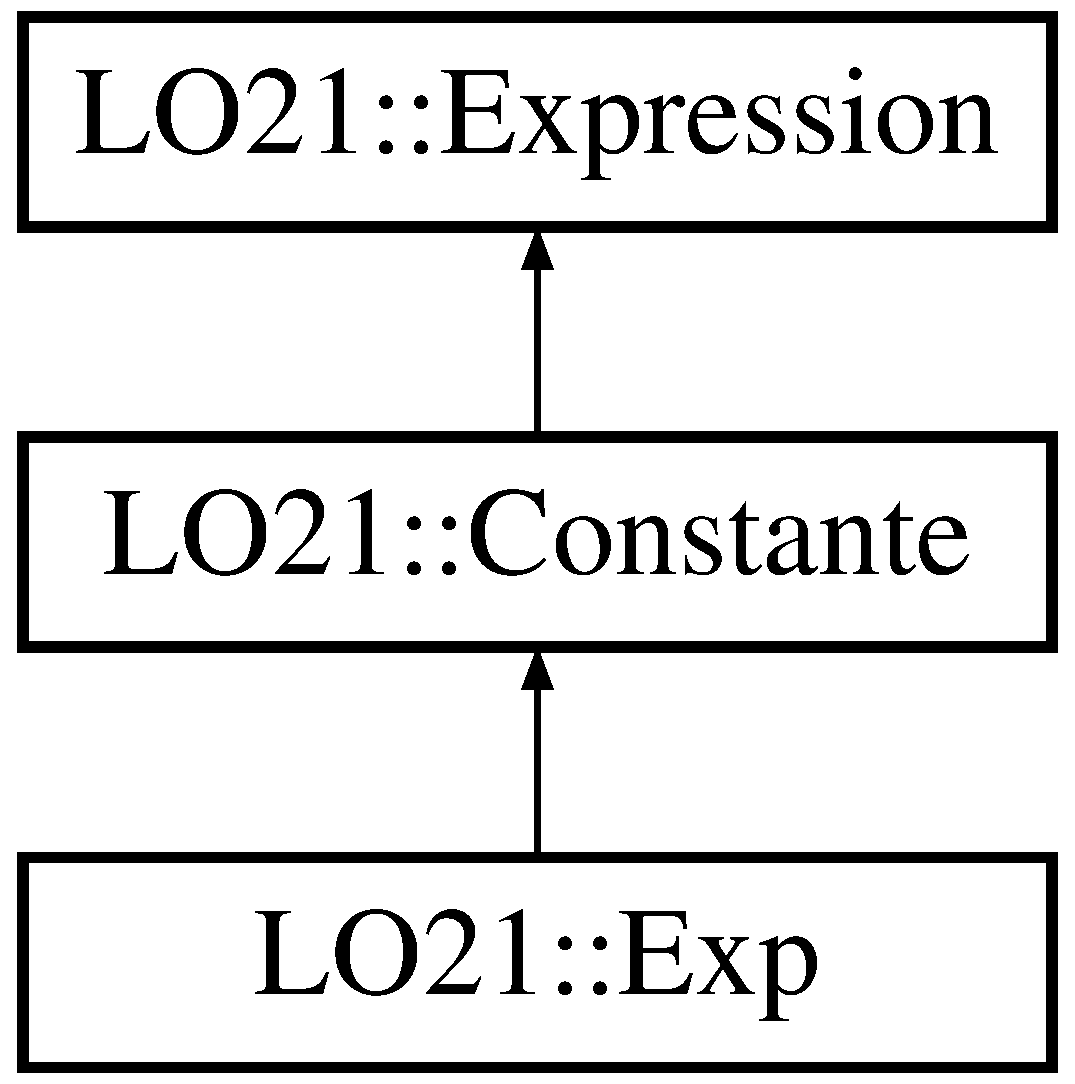
\includegraphics[height=3.000000cm]{class_l_o21_1_1_exp}
\end{center}
\end{figure}
\subsection*{\-Public \-Member \-Functions}
\begin{DoxyCompactItemize}
\item 
\hyperlink{class_l_o21_1_1_exp_a90c8e9f7a2f15a9a72423b703d5ec182}{\-Exp} (const \-Q\-String \&s)
\begin{DoxyCompactList}\small\item\em \-Constructeur de la classe \hyperlink{class_l_o21_1_1_exp}{\-Exp}. \end{DoxyCompactList}\item 
\hyperlink{class_l_o21_1_1_constante}{\-Constante} \& \hyperlink{class_l_o21_1_1_exp_afdb7c0687e2b8cda07ff85bd86299866}{addition} (const \hyperlink{class_l_o21_1_1_constante}{\-Constante} \&nb) const 
\begin{DoxyCompactList}\small\item\em \-Gere l'addition d'une constante avec l'evaluation. \end{DoxyCompactList}\item 
\hyperlink{class_l_o21_1_1_constante}{\-Constante} \& \hyperlink{class_l_o21_1_1_exp_ab4f295f8ce2768312576d76c26b6caa7}{soustraction} (const \hyperlink{class_l_o21_1_1_constante}{\-Constante} \&nb) const 
\begin{DoxyCompactList}\small\item\em \-Gere la soustraction d'une constante avec l'evaluation. \end{DoxyCompactList}\item 
\hyperlink{class_l_o21_1_1_constante}{\-Constante} \& \hyperlink{class_l_o21_1_1_exp_a6f72d9ff76fa8479d8e035eb4d1f30f0}{multiplication} (const \hyperlink{class_l_o21_1_1_constante}{\-Constante} \&nb) const 
\begin{DoxyCompactList}\small\item\em \-Gere la multiplication d'une constante avec l'evaluation. \end{DoxyCompactList}\item 
\hyperlink{class_l_o21_1_1_constante}{\-Constante} \& \hyperlink{class_l_o21_1_1_exp_ac957713a5ae0c400745b3c76a5a00eba}{division} (const \hyperlink{class_l_o21_1_1_constante}{\-Constante} \&nb) const 
\begin{DoxyCompactList}\small\item\em \-Gere la division d'une constante avec l'evaluation. \end{DoxyCompactList}\item 
\hypertarget{class_l_o21_1_1_exp_a4bf22a079395805f4e6ec3e9e254090f}{void \hyperlink{class_l_o21_1_1_exp_a4bf22a079395805f4e6ec3e9e254090f}{\-E\-V\-A\-L} ()}\label{class_l_o21_1_1_exp_a4bf22a079395805f4e6ec3e9e254090f}

\begin{DoxyCompactList}\small\item\em \-Evalue le contenu d'une expression. \end{DoxyCompactList}\item 
\hyperlink{class_l_o21_1_1_constante}{\-Constante} \& \hyperlink{class_l_o21_1_1_exp_a7733be371723e1e003b0ebf713f72124}{hook\-Operation} ()
\begin{DoxyCompactList}\small\item\em ? \end{DoxyCompactList}\item 
\-Q\-String \hyperlink{class_l_o21_1_1_exp_a89d2f21bcc4317f87d9e66809a04d2f3}{to\-String} () const 
\begin{DoxyCompactList}\small\item\em \-Permet d'afficher le contenu de l'expression. \end{DoxyCompactList}\item 
\hyperlink{class_l_o21_1_1_exp}{\-Exp} $\ast$ \hyperlink{class_l_o21_1_1_exp_ac6109efb09b218264b5a44db300bfa12}{clone} () const 
\begin{DoxyCompactList}\small\item\em \-Duplique une expression. \end{DoxyCompactList}\end{DoxyCompactItemize}


\subsection{\-Detailed \-Description}
\-Classe permettant de gerer les expressions entre ' ' a evaluer plus tard. 

\subsection{\-Constructor \& \-Destructor \-Documentation}
\hypertarget{class_l_o21_1_1_exp_a90c8e9f7a2f15a9a72423b703d5ec182}{\index{\-L\-O21\-::\-Exp@{\-L\-O21\-::\-Exp}!\-Exp@{\-Exp}}
\index{\-Exp@{\-Exp}!LO21::Exp@{\-L\-O21\-::\-Exp}}
\subsubsection[{\-Exp}]{\setlength{\rightskip}{0pt plus 5cm}{\bf \-L\-O21\-::\-Exp\-::\-Exp} (
\begin{DoxyParamCaption}
\item[{const \-Q\-String \&}]{s}
\end{DoxyParamCaption}
)\hspace{0.3cm}{\ttfamily  \mbox{[}inline\mbox{]}}}}\label{class_l_o21_1_1_exp_a90c8e9f7a2f15a9a72423b703d5ec182}


\-Constructeur de la classe \hyperlink{class_l_o21_1_1_exp}{\-Exp}. 

\hyperlink{class_l_o21_1_1_expression}{\-Expression} a garder en memoire


\begin{DoxyParams}{\-Parameters}
{\em s} & l'expression a stocker \\
\hline
\end{DoxyParams}


\subsection{\-Member \-Function \-Documentation}
\hypertarget{class_l_o21_1_1_exp_afdb7c0687e2b8cda07ff85bd86299866}{\index{\-L\-O21\-::\-Exp@{\-L\-O21\-::\-Exp}!addition@{addition}}
\index{addition@{addition}!LO21::Exp@{\-L\-O21\-::\-Exp}}
\subsubsection[{addition}]{\setlength{\rightskip}{0pt plus 5cm}{\bf \-Constante} \& {\bf \-L\-O21\-::\-Exp\-::addition} (
\begin{DoxyParamCaption}
\item[{const {\bf \-Constante} \&}]{nb}
\end{DoxyParamCaption}
) const\hspace{0.3cm}{\ttfamily  \mbox{[}virtual\mbox{]}}}}\label{class_l_o21_1_1_exp_afdb7c0687e2b8cda07ff85bd86299866}


\-Gere l'addition d'une constante avec l'evaluation. 


\begin{DoxyParams}{\-Parameters}
{\em nb} & une reference vers une constante \\
\hline
\end{DoxyParams}
\begin{DoxyReturn}{\-Returns}
\hyperlink{class_l_o21_1_1_constante}{\-Constante}\& une reference vers la constante creee a partir du resultat 
\end{DoxyReturn}


\-Implements \hyperlink{class_l_o21_1_1_constante_afbe7b10d30d13243c9e6e53c94b9bcb4}{\-L\-O21\-::\-Constante}.

\hypertarget{class_l_o21_1_1_exp_ac6109efb09b218264b5a44db300bfa12}{\index{\-L\-O21\-::\-Exp@{\-L\-O21\-::\-Exp}!clone@{clone}}
\index{clone@{clone}!LO21::Exp@{\-L\-O21\-::\-Exp}}
\subsubsection[{clone}]{\setlength{\rightskip}{0pt plus 5cm}{\bf \-Exp} $\ast$ {\bf \-L\-O21\-::\-Exp\-::clone} (
\begin{DoxyParamCaption}
{}
\end{DoxyParamCaption}
) const\hspace{0.3cm}{\ttfamily  \mbox{[}virtual\mbox{]}}}}\label{class_l_o21_1_1_exp_ac6109efb09b218264b5a44db300bfa12}


\-Duplique une expression. 

\begin{DoxyReturn}{\-Returns}
\-Exp$\ast$ un pointeur vers l'expression clonee 
\end{DoxyReturn}


\-Implements \hyperlink{class_l_o21_1_1_constante_a88ab8ec81b794ed881fba45264133aac}{\-L\-O21\-::\-Constante}.

\hypertarget{class_l_o21_1_1_exp_ac957713a5ae0c400745b3c76a5a00eba}{\index{\-L\-O21\-::\-Exp@{\-L\-O21\-::\-Exp}!division@{division}}
\index{division@{division}!LO21::Exp@{\-L\-O21\-::\-Exp}}
\subsubsection[{division}]{\setlength{\rightskip}{0pt plus 5cm}{\bf \-Constante} \& {\bf \-L\-O21\-::\-Exp\-::division} (
\begin{DoxyParamCaption}
\item[{const {\bf \-Constante} \&}]{nb}
\end{DoxyParamCaption}
) const\hspace{0.3cm}{\ttfamily  \mbox{[}virtual\mbox{]}}}}\label{class_l_o21_1_1_exp_ac957713a5ae0c400745b3c76a5a00eba}


\-Gere la division d'une constante avec l'evaluation. 


\begin{DoxyParams}{\-Parameters}
{\em nb} & une reference vers une constante \\
\hline
\end{DoxyParams}
\begin{DoxyReturn}{\-Returns}
\hyperlink{class_l_o21_1_1_constante}{\-Constante}\& une reference vers la constante creee a partir du resultat 
\end{DoxyReturn}


\-Implements \hyperlink{class_l_o21_1_1_constante_a6ffc44753a672f59272792f061c8cd55}{\-L\-O21\-::\-Constante}.

\hypertarget{class_l_o21_1_1_exp_a7733be371723e1e003b0ebf713f72124}{\index{\-L\-O21\-::\-Exp@{\-L\-O21\-::\-Exp}!hook\-Operation@{hook\-Operation}}
\index{hook\-Operation@{hook\-Operation}!LO21::Exp@{\-L\-O21\-::\-Exp}}
\subsubsection[{hook\-Operation}]{\setlength{\rightskip}{0pt plus 5cm}{\bf \-Constante} \& {\bf \-L\-O21\-::\-Exp\-::hook\-Operation} (
\begin{DoxyParamCaption}
{}
\end{DoxyParamCaption}
)\hspace{0.3cm}{\ttfamily  \mbox{[}virtual\mbox{]}}}}\label{class_l_o21_1_1_exp_a7733be371723e1e003b0ebf713f72124}


? 

\begin{DoxyReturn}{\-Returns}
\hyperlink{class_l_o21_1_1_constante}{\-Constante}\& 
\end{DoxyReturn}


\-Implements \hyperlink{class_l_o21_1_1_constante_a0e0ad1254afea74deb69a05f51220852}{\-L\-O21\-::\-Constante}.

\hypertarget{class_l_o21_1_1_exp_a6f72d9ff76fa8479d8e035eb4d1f30f0}{\index{\-L\-O21\-::\-Exp@{\-L\-O21\-::\-Exp}!multiplication@{multiplication}}
\index{multiplication@{multiplication}!LO21::Exp@{\-L\-O21\-::\-Exp}}
\subsubsection[{multiplication}]{\setlength{\rightskip}{0pt plus 5cm}{\bf \-Constante} \& {\bf \-L\-O21\-::\-Exp\-::multiplication} (
\begin{DoxyParamCaption}
\item[{const {\bf \-Constante} \&}]{nb}
\end{DoxyParamCaption}
) const\hspace{0.3cm}{\ttfamily  \mbox{[}virtual\mbox{]}}}}\label{class_l_o21_1_1_exp_a6f72d9ff76fa8479d8e035eb4d1f30f0}


\-Gere la multiplication d'une constante avec l'evaluation. 


\begin{DoxyParams}{\-Parameters}
{\em nb} & une reference vers une constante \\
\hline
\end{DoxyParams}
\begin{DoxyReturn}{\-Returns}
\hyperlink{class_l_o21_1_1_constante}{\-Constante}\& une reference vers la constante creee a partir du resultat 
\end{DoxyReturn}


\-Implements \hyperlink{class_l_o21_1_1_constante_ab2f5d581536b98c0703349fcb6536527}{\-L\-O21\-::\-Constante}.

\hypertarget{class_l_o21_1_1_exp_ab4f295f8ce2768312576d76c26b6caa7}{\index{\-L\-O21\-::\-Exp@{\-L\-O21\-::\-Exp}!soustraction@{soustraction}}
\index{soustraction@{soustraction}!LO21::Exp@{\-L\-O21\-::\-Exp}}
\subsubsection[{soustraction}]{\setlength{\rightskip}{0pt plus 5cm}{\bf \-Constante} \& {\bf \-L\-O21\-::\-Exp\-::soustraction} (
\begin{DoxyParamCaption}
\item[{const {\bf \-Constante} \&}]{nb}
\end{DoxyParamCaption}
) const\hspace{0.3cm}{\ttfamily  \mbox{[}virtual\mbox{]}}}}\label{class_l_o21_1_1_exp_ab4f295f8ce2768312576d76c26b6caa7}


\-Gere la soustraction d'une constante avec l'evaluation. 


\begin{DoxyParams}{\-Parameters}
{\em nb} & une reference vers une constante \\
\hline
\end{DoxyParams}
\begin{DoxyReturn}{\-Returns}
\hyperlink{class_l_o21_1_1_constante}{\-Constante}\& une reference vers la constante creee a partir du resultat 
\end{DoxyReturn}


\-Implements \hyperlink{class_l_o21_1_1_constante_aedf16155a16ea835c61e55c57643fa49}{\-L\-O21\-::\-Constante}.

\hypertarget{class_l_o21_1_1_exp_a89d2f21bcc4317f87d9e66809a04d2f3}{\index{\-L\-O21\-::\-Exp@{\-L\-O21\-::\-Exp}!to\-String@{to\-String}}
\index{to\-String@{to\-String}!LO21::Exp@{\-L\-O21\-::\-Exp}}
\subsubsection[{to\-String}]{\setlength{\rightskip}{0pt plus 5cm}\-Q\-String {\bf \-L\-O21\-::\-Exp\-::to\-String} (
\begin{DoxyParamCaption}
{}
\end{DoxyParamCaption}
) const\hspace{0.3cm}{\ttfamily  \mbox{[}virtual\mbox{]}}}}\label{class_l_o21_1_1_exp_a89d2f21bcc4317f87d9e66809a04d2f3}


\-Permet d'afficher le contenu de l'expression. 

\begin{DoxyReturn}{\-Returns}
\-Q\-String l'expression stockee 
\end{DoxyReturn}


\-Implements \hyperlink{class_l_o21_1_1_expression}{\-L\-O21\-::\-Expression}.



\-The documentation for this class was generated from the following files\-:\begin{DoxyCompactItemize}
\item 
\hyperlink{_exp_8h}{\-Exp.\-h}\item 
\-Exp.\-cpp\end{DoxyCompactItemize}

\hypertarget{class_l_o21_1_1_expression}{\section{\-L\-O21\-:\-:\-Expression \-Class \-Reference}
\label{class_l_o21_1_1_expression}\index{\-L\-O21\-::\-Expression@{\-L\-O21\-::\-Expression}}
}


\-Classe permettant d'encapsuler des \-Constantes et des \-Operateurs pour les stocker dans la pile.  




{\ttfamily \#include $<$\-Expression.\-h$>$}

\-Inheritance diagram for \-L\-O21\-:\-:\-Expression\-:\begin{figure}[H]
\begin{center}
\leavevmode
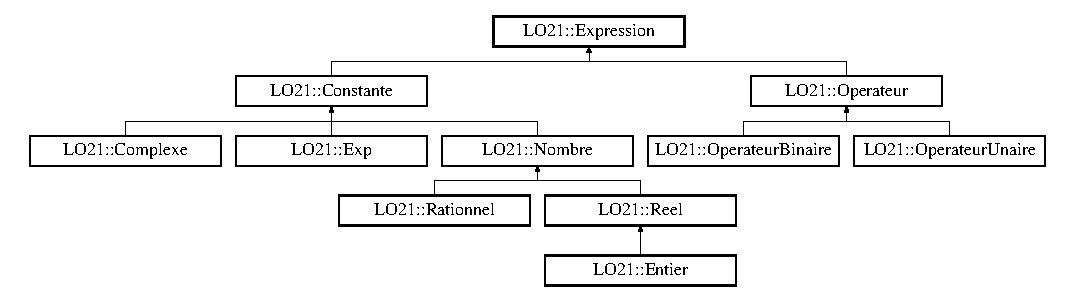
\includegraphics[height=3.612903cm]{class_l_o21_1_1_expression}
\end{center}
\end{figure}
\subsection*{\-Public \-Member \-Functions}
\begin{DoxyCompactItemize}
\item 
\hypertarget{class_l_o21_1_1_expression_a2bfd638d2010da1b60247130d24fcc13}{\hyperlink{classvirtual}{virtual} void {\bfseries \-E\-V\-A\-L} ()=0}\label{class_l_o21_1_1_expression_a2bfd638d2010da1b60247130d24fcc13}

\item 
\hypertarget{class_l_o21_1_1_expression_a067fc40ca2eb668f80420b129721b1cd}{\hyperlink{classvirtual}{virtual} \-Q\-String {\bfseries to\-String} () const =0}\label{class_l_o21_1_1_expression_a067fc40ca2eb668f80420b129721b1cd}

\item 
\hypertarget{class_l_o21_1_1_expression_ad6501101ddf87edea596d23aa85b1682}{void \hyperlink{class_l_o21_1_1_expression_ad6501101ddf87edea596d23aa85b1682}{afficher} () const }\label{class_l_o21_1_1_expression_ad6501101ddf87edea596d23aa85b1682}

\begin{DoxyCompactList}\small\item\em \-Affiche l'expression. \end{DoxyCompactList}\item 
\hyperlink{classvirtual}{virtual} \hyperlink{class_l_o21_1_1_expression}{\-Expression} $\ast$ \hyperlink{class_l_o21_1_1_expression_ad2c9e5301c976f9a2d40edaff0332715}{clone} () const =0
\begin{DoxyCompactList}\small\item\em \-Duplique un objet \hyperlink{class_l_o21_1_1_expression}{\-Expression}. \end{DoxyCompactList}\end{DoxyCompactItemize}


\subsection{\-Detailed \-Description}
\-Classe permettant d'encapsuler des \-Constantes et des \-Operateurs pour les stocker dans la pile. 

\subsection{\-Member \-Function \-Documentation}
\hypertarget{class_l_o21_1_1_expression_ad2c9e5301c976f9a2d40edaff0332715}{\index{\-L\-O21\-::\-Expression@{\-L\-O21\-::\-Expression}!clone@{clone}}
\index{clone@{clone}!LO21::Expression@{\-L\-O21\-::\-Expression}}
\subsubsection[{clone}]{\setlength{\rightskip}{0pt plus 5cm}{\bf \-Expression} $\ast$ {\bf \-L\-O21\-::\-Expression\-::clone} (
\begin{DoxyParamCaption}
{}
\end{DoxyParamCaption}
) const\hspace{0.3cm}{\ttfamily  \mbox{[}pure virtual\mbox{]}}}}\label{class_l_o21_1_1_expression_ad2c9e5301c976f9a2d40edaff0332715}


\-Duplique un objet \hyperlink{class_l_o21_1_1_expression}{\-Expression}. 

\begin{DoxyReturn}{\-Returns}
\-Expression$\ast$ un pointeur qui encapsule le reel objet duplique (\hyperlink{class_l_o21_1_1_constante}{\-Constante} ou \hyperlink{class_l_o21_1_1_operateur}{\-Operateur}) 
\end{DoxyReturn}


\-Implemented in \hyperlink{class_l_o21_1_1_nombre_aea071e3bcebfdc9337eaea8515e248c9}{\-L\-O21\-::\-Nombre}, \hyperlink{class_l_o21_1_1_complexe_a7a7a8d883e959fd7d5f84d5b2b7b2a9e}{\-L\-O21\-::\-Complexe}, \hyperlink{class_l_o21_1_1_rationnel_aab7de5f24ff5fa9f5d250e8b096ceb34}{\-L\-O21\-::\-Rationnel}, \hyperlink{class_l_o21_1_1_entier_a76f8af45d660b33c6e082986be0a9223}{\-L\-O21\-::\-Entier}, \hyperlink{class_l_o21_1_1_constante_a88ab8ec81b794ed881fba45264133aac}{\-L\-O21\-::\-Constante}, \hyperlink{class_l_o21_1_1_reel_a03bf8d59ba75b2fc45d3db330210201a}{\-L\-O21\-::\-Reel}, \hyperlink{class_l_o21_1_1_exp_ac6109efb09b218264b5a44db300bfa12}{\-L\-O21\-::\-Exp}, and \hyperlink{class_l_o21_1_1_operateur_aabf23ebda8447811b12db2f2e174b9d1}{\-L\-O21\-::\-Operateur}.



\-The documentation for this class was generated from the following file\-:\begin{DoxyCompactItemize}
\item 
\hyperlink{_expression_8h}{\-Expression.\-h}\end{DoxyCompactItemize}

\hypertarget{class_l_o21_1_1_fabrique}{\section{\-L\-O21\-:\-:\-Fabrique \-Class \-Reference}
\label{class_l_o21_1_1_fabrique}\index{\-L\-O21\-::\-Fabrique@{\-L\-O21\-::\-Fabrique}}
}


\-Classe implementant le design pattern \-Singleton, servant a decrypter la saisie utilisateur pour pouvoir instancier les bons objets.  




{\ttfamily \#include $<$\-Fabrique.\-h$>$}

\subsection*{\-Public \-Member \-Functions}
\begin{DoxyCompactItemize}
\item 
void \hyperlink{class_l_o21_1_1_fabrique_ae4a3c2c0fb11aa3a90eae748888c5279}{creer} (const \-Q\-String \&text) const 
\begin{DoxyCompactList}\small\item\em \-Parse la chaine de caractere passee en arguments et cree la classe correcte, encapsulee dans un pointeur d'\hyperlink{class_l_o21_1_1_expression}{\-Expression}, afin d'etre stockee dans la pile. \end{DoxyCompactList}\end{DoxyCompactItemize}
\subsection*{\-Static \-Public \-Member \-Functions}
\begin{DoxyCompactItemize}
\item 
static \hyperlink{class_l_o21_1_1_fabrique}{\-Fabrique} \& \hyperlink{class_l_o21_1_1_fabrique_a346ae0b4a734f429f0c51bf66ad90ccb}{get\-Instance} ()
\begin{DoxyCompactList}\small\item\em \-Permet de demander la recuperation de l'instance de \hyperlink{class_l_o21_1_1_fabrique}{\-Fabrique}, et si elle n'est pas instanciee, en creer une. \end{DoxyCompactList}\item 
\hypertarget{class_l_o21_1_1_fabrique_a4abc9c9f335269ad973781cc3018be15}{static void \hyperlink{class_l_o21_1_1_fabrique_a4abc9c9f335269ad973781cc3018be15}{libere\-Instance} ()}\label{class_l_o21_1_1_fabrique_a4abc9c9f335269ad973781cc3018be15}

\begin{DoxyCompactList}\small\item\em \-Permet de demander la destruction de l'instance de \hyperlink{class_l_o21_1_1_fabrique}{\-Fabrique}. \end{DoxyCompactList}\end{DoxyCompactItemize}


\subsection{\-Detailed \-Description}
\-Classe implementant le design pattern \-Singleton, servant a decrypter la saisie utilisateur pour pouvoir instancier les bons objets. 

\subsection{\-Member \-Function \-Documentation}
\hypertarget{class_l_o21_1_1_fabrique_ae4a3c2c0fb11aa3a90eae748888c5279}{\index{\-L\-O21\-::\-Fabrique@{\-L\-O21\-::\-Fabrique}!creer@{creer}}
\index{creer@{creer}!LO21::Fabrique@{\-L\-O21\-::\-Fabrique}}
\subsubsection[{creer}]{\setlength{\rightskip}{0pt plus 5cm}void {\bf \-L\-O21\-::\-Fabrique\-::creer} (
\begin{DoxyParamCaption}
\item[{const \-Q\-String \&}]{text}
\end{DoxyParamCaption}
) const}}\label{class_l_o21_1_1_fabrique_ae4a3c2c0fb11aa3a90eae748888c5279}


\-Parse la chaine de caractere passee en arguments et cree la classe correcte, encapsulee dans un pointeur d'\hyperlink{class_l_o21_1_1_expression}{\-Expression}, afin d'etre stockee dans la pile. 


\begin{DoxyParams}{\-Parameters}
{\em text} & la chaine a partir de laquelle les objets vont etre crees \\
\hline
\end{DoxyParams}
\hypertarget{class_l_o21_1_1_fabrique_a346ae0b4a734f429f0c51bf66ad90ccb}{\index{\-L\-O21\-::\-Fabrique@{\-L\-O21\-::\-Fabrique}!get\-Instance@{get\-Instance}}
\index{get\-Instance@{get\-Instance}!LO21::Fabrique@{\-L\-O21\-::\-Fabrique}}
\subsubsection[{get\-Instance}]{\setlength{\rightskip}{0pt plus 5cm}static {\bf \-Fabrique} \& {\bf \-L\-O21\-::\-Fabrique\-::get\-Instance} (
\begin{DoxyParamCaption}
{}
\end{DoxyParamCaption}
)\hspace{0.3cm}{\ttfamily  \mbox{[}static\mbox{]}}}}\label{class_l_o21_1_1_fabrique_a346ae0b4a734f429f0c51bf66ad90ccb}


\-Permet de demander la recuperation de l'instance de \hyperlink{class_l_o21_1_1_fabrique}{\-Fabrique}, et si elle n'est pas instanciee, en creer une. 

\begin{DoxyReturn}{\-Returns}
\hyperlink{class_l_o21_1_1_fabrique}{\-Fabrique}\& la reference vers l'instance de \hyperlink{class_l_o21_1_1_fabrique}{\-Fabrique} 
\end{DoxyReturn}


\-The documentation for this class was generated from the following files\-:\begin{DoxyCompactItemize}
\item 
\-Fabrique.\-h\item 
\-Fabrique.\-cpp\end{DoxyCompactItemize}

\hypertarget{class_l_o21_1_1_gardien}{\section{\-L\-O21\-:\-:\-Gardien \-Class \-Reference}
\label{class_l_o21_1_1_gardien}\index{\-L\-O21\-::\-Gardien@{\-L\-O21\-::\-Gardien}}
}


\-Classe qui s'occupe de gerer les operations d'undo redo grace a l'implementation d'un design pattern \-Memento.  




{\ttfamily \#include $<$\-Gardien.\-h$>$}

\subsection*{\-Public \-Member \-Functions}
\begin{DoxyCompactItemize}
\item 
void \hyperlink{class_l_o21_1_1_gardien_a893f075d068eb7cd937845c9604c069e}{ajouter\-Memento\-Undo} (\hyperlink{class_l_o21_1_1_pile_1_1_memento}{\-Pile\-::\-Memento} $\ast$p\-Memento)
\begin{DoxyCompactList}\small\item\em \-Constructeur de la classe \-Memento. \end{DoxyCompactList}\item 
void \hyperlink{class_l_o21_1_1_gardien_a01a57e73de1a335bae9d5c83465d51e3}{ajouter\-Memento\-Redo} (\hyperlink{class_l_o21_1_1_pile_1_1_memento}{\-Pile\-::\-Memento} $\ast$p\-Memento)
\begin{DoxyCompactList}\small\item\em \-Constructeur de la classe \-Memento. \end{DoxyCompactList}\item 
\hyperlink{class_l_o21_1_1_pile_1_1_memento}{\-Pile\-::\-Memento} $\ast$ \hyperlink{class_l_o21_1_1_gardien_a6abc703f1f7847d335bbf4194349082b}{get\-Memento\-Undo} ()
\begin{DoxyCompactList}\small\item\em \-Constructeur de la classe \-Memento. \end{DoxyCompactList}\item 
\hyperlink{class_l_o21_1_1_pile_1_1_memento}{\-Pile\-::\-Memento} $\ast$ \hyperlink{class_l_o21_1_1_gardien_a215a9621ff0092452a9ed46a4539988f}{get\-Memento\-Redo} ()
\begin{DoxyCompactList}\small\item\em \-Constructeur de la classe \-Memento. \end{DoxyCompactList}\item 
\hypertarget{class_l_o21_1_1_gardien_aa833c3f80e13743a175d146a6a3dca94}{void {\bfseries afficher} ()}\label{class_l_o21_1_1_gardien_aa833c3f80e13743a175d146a6a3dca94}

\item 
void \hyperlink{class_l_o21_1_1_gardien_ab2589195775b272fc05bc2de197c96be}{set\-\_\-index} (int i)
\begin{DoxyCompactList}\small\item\em \-Permet de modifier l'attribut index du \hyperlink{class_l_o21_1_1_gardien}{\-Gardien}. \end{DoxyCompactList}\end{DoxyCompactItemize}
\subsection*{\-Static \-Public \-Member \-Functions}
\begin{DoxyCompactItemize}
\item 
static \hyperlink{class_l_o21_1_1_gardien}{\-Gardien} $\ast$ \hyperlink{class_l_o21_1_1_gardien_a79253967bc5d3acf2bf110d7af6b1ed2}{get\-Instance} ()
\begin{DoxyCompactList}\small\item\em \-Recupere l'instance de l'objet \hyperlink{class_l_o21_1_1_gardien}{\-Gardien}, et s'il n'en existe pas, en cree une. \end{DoxyCompactList}\item 
\hypertarget{class_l_o21_1_1_gardien_acf2f9752ad767b1a0ae75bd718a180ac}{static void \hyperlink{class_l_o21_1_1_gardien_acf2f9752ad767b1a0ae75bd718a180ac}{libere\-Instance} ()}\label{class_l_o21_1_1_gardien_acf2f9752ad767b1a0ae75bd718a180ac}

\begin{DoxyCompactList}\small\item\em \-Demande la destruction de l'instance de la classe \hyperlink{class_l_o21_1_1_gardien}{\-Gardien}. \end{DoxyCompactList}\end{DoxyCompactItemize}


\subsection{\-Detailed \-Description}
\-Classe qui s'occupe de gerer les operations d'undo redo grace a l'implementation d'un design pattern \-Memento. 

\subsection{\-Member \-Function \-Documentation}
\hypertarget{class_l_o21_1_1_gardien_a01a57e73de1a335bae9d5c83465d51e3}{\index{\-L\-O21\-::\-Gardien@{\-L\-O21\-::\-Gardien}!ajouter\-Memento\-Redo@{ajouter\-Memento\-Redo}}
\index{ajouter\-Memento\-Redo@{ajouter\-Memento\-Redo}!LO21::Gardien@{\-L\-O21\-::\-Gardien}}
\subsubsection[{ajouter\-Memento\-Redo}]{\setlength{\rightskip}{0pt plus 5cm}void {\bf \-L\-O21\-::\-Gardien\-::ajouter\-Memento\-Redo} (
\begin{DoxyParamCaption}
\item[{{\bf \-Pile\-::\-Memento} $\ast$}]{p\-Memento}
\end{DoxyParamCaption}
)}}\label{class_l_o21_1_1_gardien_a01a57e73de1a335bae9d5c83465d51e3}


\-Constructeur de la classe \-Memento. 


\begin{DoxyParams}{\-Parameters}
{\em petat} & pointeur vers la pile actuelle a sauver en memoire \\
\hline
\end{DoxyParams}
\hypertarget{class_l_o21_1_1_gardien_a893f075d068eb7cd937845c9604c069e}{\index{\-L\-O21\-::\-Gardien@{\-L\-O21\-::\-Gardien}!ajouter\-Memento\-Undo@{ajouter\-Memento\-Undo}}
\index{ajouter\-Memento\-Undo@{ajouter\-Memento\-Undo}!LO21::Gardien@{\-L\-O21\-::\-Gardien}}
\subsubsection[{ajouter\-Memento\-Undo}]{\setlength{\rightskip}{0pt plus 5cm}void {\bf \-L\-O21\-::\-Gardien\-::ajouter\-Memento\-Undo} (
\begin{DoxyParamCaption}
\item[{{\bf \-Pile\-::\-Memento} $\ast$}]{p\-Memento}
\end{DoxyParamCaption}
)}}\label{class_l_o21_1_1_gardien_a893f075d068eb7cd937845c9604c069e}


\-Constructeur de la classe \-Memento. 


\begin{DoxyParams}{\-Parameters}
{\em petat} & pointeur vers la pile actuelle a sauver en memoire \\
\hline
\end{DoxyParams}
\hypertarget{class_l_o21_1_1_gardien_a79253967bc5d3acf2bf110d7af6b1ed2}{\index{\-L\-O21\-::\-Gardien@{\-L\-O21\-::\-Gardien}!get\-Instance@{get\-Instance}}
\index{get\-Instance@{get\-Instance}!LO21::Gardien@{\-L\-O21\-::\-Gardien}}
\subsubsection[{get\-Instance}]{\setlength{\rightskip}{0pt plus 5cm}static {\bf \-Gardien} $\ast$ {\bf \-L\-O21\-::\-Gardien\-::get\-Instance} (
\begin{DoxyParamCaption}
{}
\end{DoxyParamCaption}
)\hspace{0.3cm}{\ttfamily  \mbox{[}static\mbox{]}}}}\label{class_l_o21_1_1_gardien_a79253967bc5d3acf2bf110d7af6b1ed2}


\-Recupere l'instance de l'objet \hyperlink{class_l_o21_1_1_gardien}{\-Gardien}, et s'il n'en existe pas, en cree une. 

\begin{DoxyReturn}{\-Returns}
\-Gardien$\ast$ un pointeur vers l'objet \hyperlink{class_l_o21_1_1_gardien}{\-Gardien} surveillant l'etat de la calculatrice 
\end{DoxyReturn}
\hypertarget{class_l_o21_1_1_gardien_a215a9621ff0092452a9ed46a4539988f}{\index{\-L\-O21\-::\-Gardien@{\-L\-O21\-::\-Gardien}!get\-Memento\-Redo@{get\-Memento\-Redo}}
\index{get\-Memento\-Redo@{get\-Memento\-Redo}!LO21::Gardien@{\-L\-O21\-::\-Gardien}}
\subsubsection[{get\-Memento\-Redo}]{\setlength{\rightskip}{0pt plus 5cm}{\bf \-Pile\-::\-Memento} $\ast$ {\bf \-L\-O21\-::\-Gardien\-::get\-Memento\-Redo} (
\begin{DoxyParamCaption}
{}
\end{DoxyParamCaption}
)}}\label{class_l_o21_1_1_gardien_a215a9621ff0092452a9ed46a4539988f}


\-Constructeur de la classe \-Memento. 


\begin{DoxyParams}{\-Parameters}
{\em petat} & pointeur vers la pile actuelle a sauver en memoire \\
\hline
\end{DoxyParams}
\hypertarget{class_l_o21_1_1_gardien_a6abc703f1f7847d335bbf4194349082b}{\index{\-L\-O21\-::\-Gardien@{\-L\-O21\-::\-Gardien}!get\-Memento\-Undo@{get\-Memento\-Undo}}
\index{get\-Memento\-Undo@{get\-Memento\-Undo}!LO21::Gardien@{\-L\-O21\-::\-Gardien}}
\subsubsection[{get\-Memento\-Undo}]{\setlength{\rightskip}{0pt plus 5cm}{\bf \-Pile\-::\-Memento} $\ast$ {\bf \-L\-O21\-::\-Gardien\-::get\-Memento\-Undo} (
\begin{DoxyParamCaption}
{}
\end{DoxyParamCaption}
)}}\label{class_l_o21_1_1_gardien_a6abc703f1f7847d335bbf4194349082b}


\-Constructeur de la classe \-Memento. 


\begin{DoxyParams}{\-Parameters}
{\em petat} & pointeur vers la pile actuelle a sauver en memoire \\
\hline
\end{DoxyParams}
\hypertarget{class_l_o21_1_1_gardien_ab2589195775b272fc05bc2de197c96be}{\index{\-L\-O21\-::\-Gardien@{\-L\-O21\-::\-Gardien}!set\-\_\-index@{set\-\_\-index}}
\index{set\-\_\-index@{set\-\_\-index}!LO21::Gardien@{\-L\-O21\-::\-Gardien}}
\subsubsection[{set\-\_\-index}]{\setlength{\rightskip}{0pt plus 5cm}void {\bf \-L\-O21\-::\-Gardien\-::set\-\_\-index} (
\begin{DoxyParamCaption}
\item[{int}]{i}
\end{DoxyParamCaption}
)\hspace{0.3cm}{\ttfamily  \mbox{[}inline\mbox{]}}}}\label{class_l_o21_1_1_gardien_ab2589195775b272fc05bc2de197c96be}


\-Permet de modifier l'attribut index du \hyperlink{class_l_o21_1_1_gardien}{\-Gardien}. 


\begin{DoxyParams}{\-Parameters}
{\em i} & l'indice de la pile actuellement utilisee \\
\hline
\end{DoxyParams}


\-The documentation for this class was generated from the following files\-:\begin{DoxyCompactItemize}
\item 
\hyperlink{_gardien_8h}{\-Gardien.\-h}\item 
\-Gardien.\-cpp\end{DoxyCompactItemize}

\hypertarget{class_l_o21_1_1_log_message}{\section{\-L\-O21\-:\-:\-Log\-Message \-Class \-Reference}
\label{class_l_o21_1_1_log_message}\index{\-L\-O21\-::\-Log\-Message@{\-L\-O21\-::\-Log\-Message}}
}


\-Classe permettant de gerer l'affichage de messages informatifs.  




{\ttfamily \#include $<$\-Log\-Message.\-h$>$}

\subsection*{\-Public \-Member \-Functions}
\begin{DoxyCompactItemize}
\item 
\hyperlink{class_l_o21_1_1_log_message_a1ad22414291bccb702051bd0b1c8ff2a}{\-Log\-Message} (const \-Q\-String \&s, \hyperlink{namespace_l_o21_a129f8d204fc6d0d79283a2cf32d833df}{enum\-\_\-\-Log\-Message} i=\-I\-N\-F\-O)
\begin{DoxyCompactList}\small\item\em \-Constructeur de la classe \hyperlink{class_l_o21_1_1_log_message}{\-Log\-Message}. \end{DoxyCompactList}\item 
\-Q\-String \hyperlink{class_l_o21_1_1_log_message_a7f434101ea4728eaee6ce6c0dc6f28a7}{info} () const 
\begin{DoxyCompactList}\small\item\em \-Renvoie un message contenant les informations sur le log (date, type, message) \end{DoxyCompactList}\end{DoxyCompactItemize}


\subsection{\-Detailed \-Description}
\-Classe permettant de gerer l'affichage de messages informatifs. 

\subsection{\-Constructor \& \-Destructor \-Documentation}
\hypertarget{class_l_o21_1_1_log_message_a1ad22414291bccb702051bd0b1c8ff2a}{\index{\-L\-O21\-::\-Log\-Message@{\-L\-O21\-::\-Log\-Message}!\-Log\-Message@{\-Log\-Message}}
\index{\-Log\-Message@{\-Log\-Message}!LO21::LogMessage@{\-L\-O21\-::\-Log\-Message}}
\subsubsection[{\-Log\-Message}]{\setlength{\rightskip}{0pt plus 5cm}{\bf \-L\-O21\-::\-Log\-Message\-::\-Log\-Message} (
\begin{DoxyParamCaption}
\item[{const \-Q\-String \&}]{s, }
\item[{{\bf enum\-\_\-\-Log\-Message}}]{i = {\ttfamily \-I\-N\-F\-O}}
\end{DoxyParamCaption}
)\hspace{0.3cm}{\ttfamily  \mbox{[}inline\mbox{]}}}}\label{class_l_o21_1_1_log_message_a1ad22414291bccb702051bd0b1c8ff2a}


\-Constructeur de la classe \hyperlink{class_l_o21_1_1_log_message}{\-Log\-Message}. 

\-Type du message


\begin{DoxyParams}{\-Parameters}
{\em s} & la cha�ne de caracteres que le message affichera \\
\hline
{\em i} & le type du message \\
\hline
\end{DoxyParams}


\subsection{\-Member \-Function \-Documentation}
\hypertarget{class_l_o21_1_1_log_message_a7f434101ea4728eaee6ce6c0dc6f28a7}{\index{\-L\-O21\-::\-Log\-Message@{\-L\-O21\-::\-Log\-Message}!info@{info}}
\index{info@{info}!LO21::LogMessage@{\-L\-O21\-::\-Log\-Message}}
\subsubsection[{info}]{\setlength{\rightskip}{0pt plus 5cm}\-Q\-String {\bf \-L\-O21\-::\-Log\-Message\-::info} (
\begin{DoxyParamCaption}
{}
\end{DoxyParamCaption}
) const}}\label{class_l_o21_1_1_log_message_a7f434101ea4728eaee6ce6c0dc6f28a7}


\-Renvoie un message contenant les informations sur le log (date, type, message) 

\begin{DoxyReturn}{\-Returns}
\-Q\-String contenant la version textualisee des informations 
\end{DoxyReturn}


\-The documentation for this class was generated from the following files\-:\begin{DoxyCompactItemize}
\item 
\-Log\-Message.\-h\item 
\-Log\-Message.\-cpp\end{DoxyCompactItemize}

\hypertarget{class_l_o21_1_1_log_system}{\section{\-L\-O21\-:\-:\-Log\-System \-Class \-Reference}
\label{class_l_o21_1_1_log_system}\index{\-L\-O21\-::\-Log\-System@{\-L\-O21\-::\-Log\-System}}
}


\-Classe permettant de gerer les nombres complexes.  




{\ttfamily \#include $<$\-Log\-System.\-h$>$}

\subsection*{\-Static \-Public \-Member \-Functions}
\begin{DoxyCompactItemize}
\item 
static void \hyperlink{class_l_o21_1_1_log_system_ad6f5625c05219acbe572b3f0616e943a}{ecrire\-Console} (const \hyperlink{class_l_o21_1_1_log_message}{\-Log\-Message} \&m)
\begin{DoxyCompactList}\small\item\em \-Ecrire le message sur la console. \end{DoxyCompactList}\item 
static void \hyperlink{class_l_o21_1_1_log_system_ad6ad18df1ea2c9cb638ee562dfb76e3d}{ecrire\-Fichier} (const \hyperlink{class_l_o21_1_1_log_message}{\-Log\-Message} \&m)
\begin{DoxyCompactList}\small\item\em \-Ecrire le message dans un fichier. \end{DoxyCompactList}\item 
static void \hyperlink{class_l_o21_1_1_log_system_add7c2d0ae741eab031eb2d362c47274e}{ecrire\-Log} (const \hyperlink{class_l_o21_1_1_log_message}{\-Log\-Message} \&m)
\begin{DoxyCompactList}\small\item\em \-Permet l'appel aux deux fonctions pour ecrire dans un fichier et sur la console. \end{DoxyCompactList}\end{DoxyCompactItemize}


\subsection{\-Detailed \-Description}
\-Classe permettant de gerer les nombres complexes. 

\subsection{\-Member \-Function \-Documentation}
\hypertarget{class_l_o21_1_1_log_system_ad6f5625c05219acbe572b3f0616e943a}{\index{\-L\-O21\-::\-Log\-System@{\-L\-O21\-::\-Log\-System}!ecrire\-Console@{ecrire\-Console}}
\index{ecrire\-Console@{ecrire\-Console}!LO21::LogSystem@{\-L\-O21\-::\-Log\-System}}
\subsubsection[{ecrire\-Console}]{\setlength{\rightskip}{0pt plus 5cm}static void {\bf \-L\-O21\-::\-Log\-System\-::ecrire\-Console} (
\begin{DoxyParamCaption}
\item[{const {\bf \-Log\-Message} \&}]{m}
\end{DoxyParamCaption}
)\hspace{0.3cm}{\ttfamily  \mbox{[}static\mbox{]}}}}\label{class_l_o21_1_1_log_system_ad6f5625c05219acbe572b3f0616e943a}


\-Ecrire le message sur la console. 


\begin{DoxyParams}{\-Parameters}
{\em m} & le message a afficher \\
\hline
\end{DoxyParams}
\hypertarget{class_l_o21_1_1_log_system_ad6ad18df1ea2c9cb638ee562dfb76e3d}{\index{\-L\-O21\-::\-Log\-System@{\-L\-O21\-::\-Log\-System}!ecrire\-Fichier@{ecrire\-Fichier}}
\index{ecrire\-Fichier@{ecrire\-Fichier}!LO21::LogSystem@{\-L\-O21\-::\-Log\-System}}
\subsubsection[{ecrire\-Fichier}]{\setlength{\rightskip}{0pt plus 5cm}static void {\bf \-L\-O21\-::\-Log\-System\-::ecrire\-Fichier} (
\begin{DoxyParamCaption}
\item[{const {\bf \-Log\-Message} \&}]{m}
\end{DoxyParamCaption}
)\hspace{0.3cm}{\ttfamily  \mbox{[}static\mbox{]}}}}\label{class_l_o21_1_1_log_system_ad6ad18df1ea2c9cb638ee562dfb76e3d}


\-Ecrire le message dans un fichier. 


\begin{DoxyParams}{\-Parameters}
{\em m} & le message a afficher \\
\hline
\end{DoxyParams}
\hypertarget{class_l_o21_1_1_log_system_add7c2d0ae741eab031eb2d362c47274e}{\index{\-L\-O21\-::\-Log\-System@{\-L\-O21\-::\-Log\-System}!ecrire\-Log@{ecrire\-Log}}
\index{ecrire\-Log@{ecrire\-Log}!LO21::LogSystem@{\-L\-O21\-::\-Log\-System}}
\subsubsection[{ecrire\-Log}]{\setlength{\rightskip}{0pt plus 5cm}static void {\bf \-L\-O21\-::\-Log\-System\-::ecrire\-Log} (
\begin{DoxyParamCaption}
\item[{const {\bf \-Log\-Message} \&}]{m}
\end{DoxyParamCaption}
)\hspace{0.3cm}{\ttfamily  \mbox{[}static\mbox{]}}}}\label{class_l_o21_1_1_log_system_add7c2d0ae741eab031eb2d362c47274e}


\-Permet l'appel aux deux fonctions pour ecrire dans un fichier et sur la console. 


\begin{DoxyParams}{\-Parameters}
{\em m} & le message a afficher \\
\hline
\end{DoxyParams}


\-The documentation for this class was generated from the following files\-:\begin{DoxyCompactItemize}
\item 
\-Log\-System.\-h\item 
\-Log\-System.\-cpp\end{DoxyCompactItemize}

\hypertarget{class_main_window}{\section{\-Main\-Window \-Class \-Reference}
\label{class_main_window}\index{\-Main\-Window@{\-Main\-Window}}
}
\subsection*{\-Public \-Member \-Functions}
\begin{DoxyCompactItemize}
\item 
\hypertarget{class_main_window_a8b244be8b7b7db1b08de2a2acb9409db}{{\bfseries \-Main\-Window} (\-Q\-Widget $\ast$parent=0)}\label{class_main_window_a8b244be8b7b7db1b08de2a2acb9409db}

\end{DoxyCompactItemize}


\-The documentation for this class was generated from the following files\-:\begin{DoxyCompactItemize}
\item 
\hyperlink{mainwindow_8h}{mainwindow.\-h}\item 
mainwindow.\-cpp\end{DoxyCompactItemize}

\hypertarget{class_l_o21_1_1_pile_1_1_memento}{\section{\-L\-O21\-:\-:\-Pile\-:\-:\-Memento \-Class \-Reference}
\label{class_l_o21_1_1_pile_1_1_memento}\index{\-L\-O21\-::\-Pile\-::\-Memento@{\-L\-O21\-::\-Pile\-::\-Memento}}
}


\-Classe permettant de gerer divers etats d'un meme objet.  




{\ttfamily \#include $<$\-Pile.\-h$>$}

\subsection*{\-Public \-Member \-Functions}
\begin{DoxyCompactItemize}
\item 
\hyperlink{class_l_o21_1_1_pile_1_1_memento_a494b30790ff93d10f3291bd3ccc8f591}{\-Memento} (const \hyperlink{class_l_o21_1_1_pile}{\-Pile} $\ast$petat)
\begin{DoxyCompactList}\small\item\em \-Constructeur de la classe \hyperlink{class_l_o21_1_1_pile_1_1_memento}{\-Memento}. \end{DoxyCompactList}\item 
\hyperlink{class_l_o21_1_1_pile}{\-Pile} $\ast$ \hyperlink{class_l_o21_1_1_pile_1_1_memento_a69c6f76d7b3cf1bf10b811aac48037fc}{get\-\_\-etat} () const 
\begin{DoxyCompactList}\small\item\em \-Retourne l'etat sauvegarde de la pile. \end{DoxyCompactList}\end{DoxyCompactItemize}


\subsection{\-Detailed \-Description}
\-Classe permettant de gerer divers etats d'un meme objet. 

\subsection{\-Constructor \& \-Destructor \-Documentation}
\hypertarget{class_l_o21_1_1_pile_1_1_memento_a494b30790ff93d10f3291bd3ccc8f591}{\index{\-L\-O21\-::\-Pile\-::\-Memento@{\-L\-O21\-::\-Pile\-::\-Memento}!\-Memento@{\-Memento}}
\index{\-Memento@{\-Memento}!LO21::Pile::Memento@{\-L\-O21\-::\-Pile\-::\-Memento}}
\subsubsection[{\-Memento}]{\setlength{\rightskip}{0pt plus 5cm}{\bf \-L\-O21\-::\-Pile\-::\-Memento\-::\-Memento} (
\begin{DoxyParamCaption}
\item[{const {\bf \-Pile} $\ast$}]{petat}
\end{DoxyParamCaption}
)\hspace{0.3cm}{\ttfamily  \mbox{[}inline\mbox{]}}}}\label{class_l_o21_1_1_pile_1_1_memento_a494b30790ff93d10f3291bd3ccc8f591}


\-Constructeur de la classe \hyperlink{class_l_o21_1_1_pile_1_1_memento}{\-Memento}. 

\-La pile dont on veut garder l'etat en memoire


\begin{DoxyParams}{\-Parameters}
{\em petat} & pointeur vers la pile actuelle a sauver en memoire \\
\hline
\end{DoxyParams}


\subsection{\-Member \-Function \-Documentation}
\hypertarget{class_l_o21_1_1_pile_1_1_memento_a69c6f76d7b3cf1bf10b811aac48037fc}{\index{\-L\-O21\-::\-Pile\-::\-Memento@{\-L\-O21\-::\-Pile\-::\-Memento}!get\-\_\-etat@{get\-\_\-etat}}
\index{get\-\_\-etat@{get\-\_\-etat}!LO21::Pile::Memento@{\-L\-O21\-::\-Pile\-::\-Memento}}
\subsubsection[{get\-\_\-etat}]{\setlength{\rightskip}{0pt plus 5cm}{\bf \-Pile} $\ast$ {\bf \-L\-O21\-::\-Pile\-::\-Memento\-::get\-\_\-etat} (
\begin{DoxyParamCaption}
{}
\end{DoxyParamCaption}
) const\hspace{0.3cm}{\ttfamily  \mbox{[}inline\mbox{]}}}}\label{class_l_o21_1_1_pile_1_1_memento_a69c6f76d7b3cf1bf10b811aac48037fc}


\-Retourne l'etat sauvegarde de la pile. 

\begin{DoxyReturn}{\-Returns}
\-Pile$\ast$ pointeur vers la pile sauvegardee 
\end{DoxyReturn}


\-The documentation for this class was generated from the following file\-:\begin{DoxyCompactItemize}
\item 
\hyperlink{_pile_8h}{\-Pile.\-h}\end{DoxyCompactItemize}

\hypertarget{class_l_o21_1_1_nombre}{\section{\-L\-O21\-:\-:\-Nombre \-Class \-Reference}
\label{class_l_o21_1_1_nombre}\index{\-L\-O21\-::\-Nombre@{\-L\-O21\-::\-Nombre}}
}


\-Classe encapsulant les classes \hyperlink{class_l_o21_1_1_entier}{\-Entier}, \hyperlink{class_l_o21_1_1_rationnel}{\-Rationnel} et \hyperlink{class_l_o21_1_1_reel}{\-Reel}.  




{\ttfamily \#include $<$\-Nombre.\-h$>$}

\-Inheritance diagram for \-L\-O21\-:\-:\-Nombre\-:\begin{figure}[H]
\begin{center}
\leavevmode
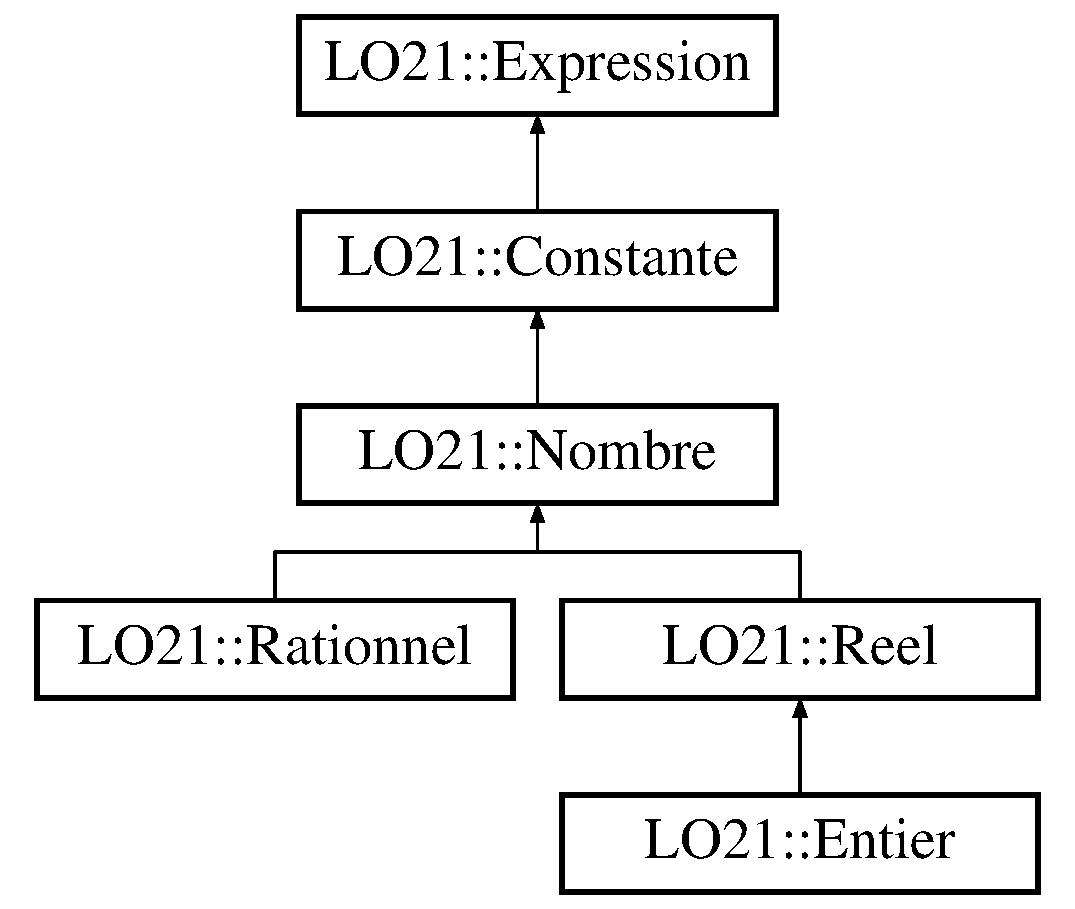
\includegraphics[height=5.000000cm]{class_l_o21_1_1_nombre}
\end{center}
\end{figure}
\subsection*{\-Public \-Member \-Functions}
\begin{DoxyCompactItemize}
\item 
\hyperlink{classvirtual}{virtual} \hyperlink{class_l_o21_1_1_constante}{\-Constante} \& \hyperlink{class_l_o21_1_1_nombre_abf009b9533e0d24f76944ba49372ff52}{\-S\-I\-N} () const 
\begin{DoxyCompactList}\small\item\em \-Calcule le sinus du nombre. \end{DoxyCompactList}\item 
\hyperlink{classvirtual}{virtual} \hyperlink{class_l_o21_1_1_constante}{\-Constante} \& \hyperlink{class_l_o21_1_1_nombre_a791656eaee79d02632d4c9a771c21d3f}{\-C\-O\-S} () const 
\begin{DoxyCompactList}\small\item\em \-Calcule le cosinus du nombre. \end{DoxyCompactList}\item 
\hyperlink{classvirtual}{virtual} \hyperlink{class_l_o21_1_1_constante}{\-Constante} \& \hyperlink{class_l_o21_1_1_nombre_a3281daef643e38927c06ef87ac0d16f9}{\-T\-A\-N} () const 
\begin{DoxyCompactList}\small\item\em \-Calcule la tangente du nombre. \end{DoxyCompactList}\item 
\hyperlink{classvirtual}{virtual} \hyperlink{class_l_o21_1_1_constante}{\-Constante} \& \hyperlink{class_l_o21_1_1_nombre_a551edca4f98fb71ba2b634d8cc2b9b0b}{\-S\-I\-N\-H} () const 
\begin{DoxyCompactList}\small\item\em \-Calcule le sinus hyperbolique du nombre. \end{DoxyCompactList}\item 
\hyperlink{classvirtual}{virtual} \hyperlink{class_l_o21_1_1_constante}{\-Constante} \& \hyperlink{class_l_o21_1_1_nombre_a9c944c852c27897718a54aca53e92bec}{\-C\-O\-S\-H} () const 
\begin{DoxyCompactList}\small\item\em \-Calcule le cosinus hyperbolique du nombre. \end{DoxyCompactList}\item 
\hyperlink{classvirtual}{virtual} \hyperlink{class_l_o21_1_1_constante}{\-Constante} \& \hyperlink{class_l_o21_1_1_nombre_a3085b62b3e4605b7f62cb824aff5309f}{\-T\-A\-N\-H} () const 
\begin{DoxyCompactList}\small\item\em \-Calcule la tangente hyperbolique du nombre. \end{DoxyCompactList}\item 
\hyperlink{classvirtual}{virtual} \hyperlink{class_l_o21_1_1_constante}{\-Constante} \& \hyperlink{class_l_o21_1_1_nombre_aa66572023ae408b6b2c8fc6babe2b9c9}{\-L\-N} () const 
\begin{DoxyCompactList}\small\item\em \-Calcule le logarithme neperien du nombre. \end{DoxyCompactList}\item 
\hyperlink{classvirtual}{virtual} \hyperlink{class_l_o21_1_1_constante}{\-Constante} \& \hyperlink{class_l_o21_1_1_nombre_aad5958e0b3583453b548e8369470a77f}{\-L\-O\-G} () const 
\begin{DoxyCompactList}\small\item\em \-Calcule le logarithme du nombre. \end{DoxyCompactList}\item 
\hyperlink{classvirtual}{virtual} \hyperlink{class_l_o21_1_1_constante}{\-Constante} \& \hyperlink{class_l_o21_1_1_nombre_a143b8821200279ae56a13531c94d891f}{\-I\-N\-V} () const 
\begin{DoxyCompactList}\small\item\em \-Calcule l'inverse du nombre. \end{DoxyCompactList}\item 
\hyperlink{classvirtual}{virtual} \hyperlink{class_l_o21_1_1_constante}{\-Constante} \& \hyperlink{class_l_o21_1_1_nombre_adac454c03cc80ab403fe1346e067be0b}{\-S\-Q\-R\-T} () const 
\begin{DoxyCompactList}\small\item\em \-Calcule la racine carre du nombre. \end{DoxyCompactList}\item 
\hyperlink{classvirtual}{virtual} \hyperlink{class_l_o21_1_1_constante}{\-Constante} \& \hyperlink{class_l_o21_1_1_nombre_a80021d921a8519d3548a11b2d6acea7d}{\-P\-O\-W} (const \hyperlink{class_l_o21_1_1_nombre}{\-Nombre} \&nb) const 
\begin{DoxyCompactList}\small\item\em \-Calcule le nombre a la puissance passee en argument. \end{DoxyCompactList}\item 
\hyperlink{classvirtual}{virtual} \hyperlink{class_l_o21_1_1_entier}{\-Entier} \& \hyperlink{class_l_o21_1_1_nombre_a50ad2148d1f0de749361329268117a25}{to\-Entier} () const 
\begin{DoxyCompactList}\small\item\em \-Transforme un \hyperlink{class_l_o21_1_1_nombre}{\-Nombre} en entier. \end{DoxyCompactList}\item 
\hyperlink{classvirtual}{virtual} \hyperlink{class_l_o21_1_1_reel}{\-Reel} \& \hyperlink{class_l_o21_1_1_nombre_a778c4e954d3bfb9a226b4fb618441a56}{to\-Reel} () const 
\begin{DoxyCompactList}\small\item\em \-Transforme un \hyperlink{class_l_o21_1_1_nombre}{\-Nombre} en reel. \end{DoxyCompactList}\item 
\hyperlink{classvirtual}{virtual} \hyperlink{class_l_o21_1_1_rationnel}{\-Rationnel} \& \hyperlink{class_l_o21_1_1_nombre_a89c9efd6230695a6ace9605a2a82ee96}{to\-Rationnel} () const 
\begin{DoxyCompactList}\small\item\em \-Transforme un \hyperlink{class_l_o21_1_1_nombre}{\-Nombre} en rationnel. \end{DoxyCompactList}\item 
\-Q\-String \hyperlink{class_l_o21_1_1_nombre_a081a338b80d4f51048c0729597708c24}{to\-String} () const =0
\begin{DoxyCompactList}\small\item\em \-Methode virtuelle servant a donner une representation textuelle d'un nombre. \end{DoxyCompactList}\item 
\hyperlink{class_l_o21_1_1_nombre}{\-Nombre} \& \hyperlink{class_l_o21_1_1_nombre_ac420c18d67faf83c1e0751be1c69579d}{\-S\-I\-G\-N} () const 
\begin{DoxyCompactList}\small\item\em \-Inverse le signe d'un nombre. \end{DoxyCompactList}\item 
\hyperlink{classvirtual}{virtual} \hyperlink{class_l_o21_1_1_constante}{\-Constante} \& \hyperlink{class_l_o21_1_1_nombre_a75c7a5c063ed122f7ba004e09f1f6621}{addition} (const \hyperlink{class_l_o21_1_1_constante}{\-Constante} \&nb) const =0
\begin{DoxyCompactList}\small\item\em \-Gere l'addition entre deux constantes quelles qu'elles soient. \end{DoxyCompactList}\item 
\hyperlink{classvirtual}{virtual} \hyperlink{class_l_o21_1_1_constante}{\-Constante} \& \hyperlink{class_l_o21_1_1_nombre_a1e412b0e89c0b68c0ee04a3078c098b1}{soustraction} (const \hyperlink{class_l_o21_1_1_constante}{\-Constante} \&nb) const =0
\begin{DoxyCompactList}\small\item\em \-Gere la soustraction entre deux constantes quelles qu'elles soient. \end{DoxyCompactList}\item 
\hyperlink{classvirtual}{virtual} \hyperlink{class_l_o21_1_1_constante}{\-Constante} \& \hyperlink{class_l_o21_1_1_nombre_a63cf8dbd304585fe106e8eeebe8c4e89}{multiplication} (const \hyperlink{class_l_o21_1_1_constante}{\-Constante} \&nb) const =0
\begin{DoxyCompactList}\small\item\em \-Gere la multiplication entre deux constantes quelles qu'elles soient. \end{DoxyCompactList}\item 
\hyperlink{classvirtual}{virtual} \hyperlink{class_l_o21_1_1_constante}{\-Constante} \& \hyperlink{class_l_o21_1_1_nombre_aafde3453c22512a8ca152f4013d0f08f}{division} (const \hyperlink{class_l_o21_1_1_constante}{\-Constante} \&nb) const =0
\begin{DoxyCompactList}\small\item\em \-Gere la division entre deux constantes quelles qu'elles soient. \end{DoxyCompactList}\item 
\hyperlink{class_l_o21_1_1_constante}{\-Constante} \& \hyperlink{class_l_o21_1_1_nombre_a27247b37ee0159071efbd64bc73d852c}{hook\-Operation} ()
\begin{DoxyCompactList}\small\item\em \-Permet de vérifier le type d'opération et de constante pour instancier correctement un objet. \end{DoxyCompactList}\item 
bool \hyperlink{class_l_o21_1_1_nombre_a13d1275bac5b339723ee7b033461c9a4}{operator==} (const \hyperlink{class_l_o21_1_1_nombre}{\-Nombre} \&nb) const 
\begin{DoxyCompactList}\small\item\em \-Teste si la valeur d'un \hyperlink{class_l_o21_1_1_nombre}{\-Nombre} est egale a la valeur d'un autre \hyperlink{class_l_o21_1_1_nombre}{\-Nombre}. \end{DoxyCompactList}\item 
bool \hyperlink{class_l_o21_1_1_nombre_ab0d95d7d706e176ee9121feecacf3be7}{operator==} (int nb) const 
\begin{DoxyCompactList}\small\item\em \-Teste si la valeur d'un \hyperlink{class_l_o21_1_1_nombre}{\-Nombre} est egale a la valeur d'un entier. \end{DoxyCompactList}\item 
\hyperlink{class_l_o21_1_1_nombre}{\-Nombre} $\ast$ \hyperlink{class_l_o21_1_1_nombre_aea071e3bcebfdc9337eaea8515e248c9}{clone} () const =0
\begin{DoxyCompactList}\small\item\em \-Recopie le nombre appelant. \end{DoxyCompactList}\end{DoxyCompactItemize}


\subsection{\-Detailed \-Description}
\-Classe encapsulant les classes \hyperlink{class_l_o21_1_1_entier}{\-Entier}, \hyperlink{class_l_o21_1_1_rationnel}{\-Rationnel} et \hyperlink{class_l_o21_1_1_reel}{\-Reel}. 

\subsection{\-Member \-Function \-Documentation}
\hypertarget{class_l_o21_1_1_nombre_a75c7a5c063ed122f7ba004e09f1f6621}{\index{\-L\-O21\-::\-Nombre@{\-L\-O21\-::\-Nombre}!addition@{addition}}
\index{addition@{addition}!LO21::Nombre@{\-L\-O21\-::\-Nombre}}
\subsubsection[{addition}]{\setlength{\rightskip}{0pt plus 5cm}{\bf \-Constante} \& {\bf \-L\-O21\-::\-Nombre\-::addition} (
\begin{DoxyParamCaption}
\item[{const {\bf \-Constante} \&}]{nb}
\end{DoxyParamCaption}
) const\hspace{0.3cm}{\ttfamily  \mbox{[}pure virtual\mbox{]}}}}\label{class_l_o21_1_1_nombre_a75c7a5c063ed122f7ba004e09f1f6621}


\-Gere l'addition entre deux constantes quelles qu'elles soient. 


\begin{DoxyParams}{\-Parameters}
{\em nb} & une reference vers une constante \\
\hline
\end{DoxyParams}
\begin{DoxyReturn}{\-Returns}
\hyperlink{class_l_o21_1_1_constante}{\-Constante}\& une reference vers la constante creee a partir du resultat 
\end{DoxyReturn}


\-Implements \hyperlink{class_l_o21_1_1_constante_afbe7b10d30d13243c9e6e53c94b9bcb4}{\-L\-O21\-::\-Constante}.



\-Implemented in \hyperlink{class_l_o21_1_1_reel_ada705f00ece11942f330bad8497c2cb5}{\-L\-O21\-::\-Reel}, \hyperlink{class_l_o21_1_1_entier_a8c70a23f95a29034d78fc5b8c76c4265}{\-L\-O21\-::\-Entier}, and \hyperlink{class_l_o21_1_1_rationnel_a67e3dea6269482abdf3101e16e53c769}{\-L\-O21\-::\-Rationnel}.

\hypertarget{class_l_o21_1_1_nombre_aea071e3bcebfdc9337eaea8515e248c9}{\index{\-L\-O21\-::\-Nombre@{\-L\-O21\-::\-Nombre}!clone@{clone}}
\index{clone@{clone}!LO21::Nombre@{\-L\-O21\-::\-Nombre}}
\subsubsection[{clone}]{\setlength{\rightskip}{0pt plus 5cm}{\bf \-Nombre} $\ast$ {\bf \-L\-O21\-::\-Nombre\-::clone} (
\begin{DoxyParamCaption}
{}
\end{DoxyParamCaption}
) const\hspace{0.3cm}{\ttfamily  \mbox{[}pure virtual\mbox{]}}}}\label{class_l_o21_1_1_nombre_aea071e3bcebfdc9337eaea8515e248c9}


\-Recopie le nombre appelant. 

\begin{DoxyReturn}{\-Returns}
\-Nombre$\ast$ un pointeur vers le nombre cree par recopie 
\end{DoxyReturn}


\-Implements \hyperlink{class_l_o21_1_1_constante_a88ab8ec81b794ed881fba45264133aac}{\-L\-O21\-::\-Constante}.



\-Implemented in \hyperlink{class_l_o21_1_1_rationnel_aab7de5f24ff5fa9f5d250e8b096ceb34}{\-L\-O21\-::\-Rationnel}, \hyperlink{class_l_o21_1_1_entier_a76f8af45d660b33c6e082986be0a9223}{\-L\-O21\-::\-Entier}, and \hyperlink{class_l_o21_1_1_reel_a03bf8d59ba75b2fc45d3db330210201a}{\-L\-O21\-::\-Reel}.

\hypertarget{class_l_o21_1_1_nombre_a791656eaee79d02632d4c9a771c21d3f}{\index{\-L\-O21\-::\-Nombre@{\-L\-O21\-::\-Nombre}!\-C\-O\-S@{\-C\-O\-S}}
\index{\-C\-O\-S@{\-C\-O\-S}!LO21::Nombre@{\-L\-O21\-::\-Nombre}}
\subsubsection[{\-C\-O\-S}]{\setlength{\rightskip}{0pt plus 5cm}{\bf \-Constante} \& {\bf \-L\-O21\-::\-Nombre\-::\-C\-O\-S} (
\begin{DoxyParamCaption}
{}
\end{DoxyParamCaption}
) const\hspace{0.3cm}{\ttfamily  \mbox{[}virtual\mbox{]}}}}\label{class_l_o21_1_1_nombre_a791656eaee79d02632d4c9a771c21d3f}


\-Calcule le cosinus du nombre. 

\begin{DoxyReturn}{\-Returns}
\hyperlink{class_l_o21_1_1_constante}{\-Constante}\& une reference vers la constante issue du resultat 
\end{DoxyReturn}
\hypertarget{class_l_o21_1_1_nombre_a9c944c852c27897718a54aca53e92bec}{\index{\-L\-O21\-::\-Nombre@{\-L\-O21\-::\-Nombre}!\-C\-O\-S\-H@{\-C\-O\-S\-H}}
\index{\-C\-O\-S\-H@{\-C\-O\-S\-H}!LO21::Nombre@{\-L\-O21\-::\-Nombre}}
\subsubsection[{\-C\-O\-S\-H}]{\setlength{\rightskip}{0pt plus 5cm}{\bf \-Constante} \& {\bf \-L\-O21\-::\-Nombre\-::\-C\-O\-S\-H} (
\begin{DoxyParamCaption}
{}
\end{DoxyParamCaption}
) const\hspace{0.3cm}{\ttfamily  \mbox{[}virtual\mbox{]}}}}\label{class_l_o21_1_1_nombre_a9c944c852c27897718a54aca53e92bec}


\-Calcule le cosinus hyperbolique du nombre. 

\begin{DoxyReturn}{\-Returns}
\hyperlink{class_l_o21_1_1_constante}{\-Constante}\& une reference vers la constante issue du resultat 
\end{DoxyReturn}
\hypertarget{class_l_o21_1_1_nombre_aafde3453c22512a8ca152f4013d0f08f}{\index{\-L\-O21\-::\-Nombre@{\-L\-O21\-::\-Nombre}!division@{division}}
\index{division@{division}!LO21::Nombre@{\-L\-O21\-::\-Nombre}}
\subsubsection[{division}]{\setlength{\rightskip}{0pt plus 5cm}{\bf \-Constante} \& {\bf \-L\-O21\-::\-Nombre\-::division} (
\begin{DoxyParamCaption}
\item[{const {\bf \-Constante} \&}]{nb}
\end{DoxyParamCaption}
) const\hspace{0.3cm}{\ttfamily  \mbox{[}pure virtual\mbox{]}}}}\label{class_l_o21_1_1_nombre_aafde3453c22512a8ca152f4013d0f08f}


\-Gere la division entre deux constantes quelles qu'elles soient. 


\begin{DoxyParams}{\-Parameters}
{\em nb} & une reference vers une constante \\
\hline
\end{DoxyParams}
\begin{DoxyReturn}{\-Returns}
\hyperlink{class_l_o21_1_1_constante}{\-Constante}\& une reference vers la constante creee a partir du resultat 
\end{DoxyReturn}


\-Implements \hyperlink{class_l_o21_1_1_constante_a6ffc44753a672f59272792f061c8cd55}{\-L\-O21\-::\-Constante}.



\-Implemented in \hyperlink{class_l_o21_1_1_reel_a2b4c6ae1d997ddd4e32e10e4511cfae0}{\-L\-O21\-::\-Reel}, \hyperlink{class_l_o21_1_1_entier_a4a9e09753bde4c527596c9a2cda8c87e}{\-L\-O21\-::\-Entier}, and \hyperlink{class_l_o21_1_1_rationnel_abc26382a7434c12b941e8c68547985c4}{\-L\-O21\-::\-Rationnel}.

\hypertarget{class_l_o21_1_1_nombre_a27247b37ee0159071efbd64bc73d852c}{\index{\-L\-O21\-::\-Nombre@{\-L\-O21\-::\-Nombre}!hook\-Operation@{hook\-Operation}}
\index{hook\-Operation@{hook\-Operation}!LO21::Nombre@{\-L\-O21\-::\-Nombre}}
\subsubsection[{hook\-Operation}]{\setlength{\rightskip}{0pt plus 5cm}{\bf \-Constante} \& {\bf \-L\-O21\-::\-Nombre\-::hook\-Operation} (
\begin{DoxyParamCaption}
{}
\end{DoxyParamCaption}
)\hspace{0.3cm}{\ttfamily  \mbox{[}virtual\mbox{]}}}}\label{class_l_o21_1_1_nombre_a27247b37ee0159071efbd64bc73d852c}


\-Permet de vérifier le type d'opération et de constante pour instancier correctement un objet. 

\begin{DoxyReturn}{\-Returns}
\hyperlink{class_l_o21_1_1_constante}{\-Constante}\& \-Une reference vers une constante instanciee 
\end{DoxyReturn}


\-Implements \hyperlink{class_l_o21_1_1_constante_a0e0ad1254afea74deb69a05f51220852}{\-L\-O21\-::\-Constante}.

\hypertarget{class_l_o21_1_1_nombre_a143b8821200279ae56a13531c94d891f}{\index{\-L\-O21\-::\-Nombre@{\-L\-O21\-::\-Nombre}!\-I\-N\-V@{\-I\-N\-V}}
\index{\-I\-N\-V@{\-I\-N\-V}!LO21::Nombre@{\-L\-O21\-::\-Nombre}}
\subsubsection[{\-I\-N\-V}]{\setlength{\rightskip}{0pt plus 5cm}{\bf \-Constante} \& {\bf \-L\-O21\-::\-Nombre\-::\-I\-N\-V} (
\begin{DoxyParamCaption}
{}
\end{DoxyParamCaption}
) const\hspace{0.3cm}{\ttfamily  \mbox{[}virtual\mbox{]}}}}\label{class_l_o21_1_1_nombre_a143b8821200279ae56a13531c94d891f}


\-Calcule l'inverse du nombre. 

\begin{DoxyReturn}{\-Returns}
\hyperlink{class_l_o21_1_1_constante}{\-Constante}\& une reference vers la constante issue du resultat 
\end{DoxyReturn}
\hypertarget{class_l_o21_1_1_nombre_aa66572023ae408b6b2c8fc6babe2b9c9}{\index{\-L\-O21\-::\-Nombre@{\-L\-O21\-::\-Nombre}!\-L\-N@{\-L\-N}}
\index{\-L\-N@{\-L\-N}!LO21::Nombre@{\-L\-O21\-::\-Nombre}}
\subsubsection[{\-L\-N}]{\setlength{\rightskip}{0pt plus 5cm}{\bf \-Constante} \& {\bf \-L\-O21\-::\-Nombre\-::\-L\-N} (
\begin{DoxyParamCaption}
{}
\end{DoxyParamCaption}
) const\hspace{0.3cm}{\ttfamily  \mbox{[}virtual\mbox{]}}}}\label{class_l_o21_1_1_nombre_aa66572023ae408b6b2c8fc6babe2b9c9}


\-Calcule le logarithme neperien du nombre. 

\begin{DoxyReturn}{\-Returns}
\hyperlink{class_l_o21_1_1_constante}{\-Constante}\& une reference vers la constante issue du resultat 
\end{DoxyReturn}
\hypertarget{class_l_o21_1_1_nombre_aad5958e0b3583453b548e8369470a77f}{\index{\-L\-O21\-::\-Nombre@{\-L\-O21\-::\-Nombre}!\-L\-O\-G@{\-L\-O\-G}}
\index{\-L\-O\-G@{\-L\-O\-G}!LO21::Nombre@{\-L\-O21\-::\-Nombre}}
\subsubsection[{\-L\-O\-G}]{\setlength{\rightskip}{0pt plus 5cm}{\bf \-Constante} \& {\bf \-L\-O21\-::\-Nombre\-::\-L\-O\-G} (
\begin{DoxyParamCaption}
{}
\end{DoxyParamCaption}
) const\hspace{0.3cm}{\ttfamily  \mbox{[}virtual\mbox{]}}}}\label{class_l_o21_1_1_nombre_aad5958e0b3583453b548e8369470a77f}


\-Calcule le logarithme du nombre. 

\begin{DoxyReturn}{\-Returns}
\hyperlink{class_l_o21_1_1_constante}{\-Constante}\& une reference vers la constante issue du resultat 
\end{DoxyReturn}
\hypertarget{class_l_o21_1_1_nombre_a63cf8dbd304585fe106e8eeebe8c4e89}{\index{\-L\-O21\-::\-Nombre@{\-L\-O21\-::\-Nombre}!multiplication@{multiplication}}
\index{multiplication@{multiplication}!LO21::Nombre@{\-L\-O21\-::\-Nombre}}
\subsubsection[{multiplication}]{\setlength{\rightskip}{0pt plus 5cm}{\bf \-Constante} \& {\bf \-L\-O21\-::\-Nombre\-::multiplication} (
\begin{DoxyParamCaption}
\item[{const {\bf \-Constante} \&}]{nb}
\end{DoxyParamCaption}
) const\hspace{0.3cm}{\ttfamily  \mbox{[}pure virtual\mbox{]}}}}\label{class_l_o21_1_1_nombre_a63cf8dbd304585fe106e8eeebe8c4e89}


\-Gere la multiplication entre deux constantes quelles qu'elles soient. 


\begin{DoxyParams}{\-Parameters}
{\em nb} & une reference vers une constante \\
\hline
\end{DoxyParams}
\begin{DoxyReturn}{\-Returns}
\hyperlink{class_l_o21_1_1_constante}{\-Constante}\& une reference vers la constante creee a partir du resultat 
\end{DoxyReturn}


\-Implements \hyperlink{class_l_o21_1_1_constante_ab2f5d581536b98c0703349fcb6536527}{\-L\-O21\-::\-Constante}.



\-Implemented in \hyperlink{class_l_o21_1_1_reel_a01e5dc973684a30f98f7bde0d0c5840d}{\-L\-O21\-::\-Reel}, \hyperlink{class_l_o21_1_1_entier_a34fdbc8acc0a18318916312983dc78f9}{\-L\-O21\-::\-Entier}, and \hyperlink{class_l_o21_1_1_rationnel_ad59a24eab43b40d59e639078a9a9d638}{\-L\-O21\-::\-Rationnel}.

\hypertarget{class_l_o21_1_1_nombre_a13d1275bac5b339723ee7b033461c9a4}{\index{\-L\-O21\-::\-Nombre@{\-L\-O21\-::\-Nombre}!operator==@{operator==}}
\index{operator==@{operator==}!LO21::Nombre@{\-L\-O21\-::\-Nombre}}
\subsubsection[{operator==}]{\setlength{\rightskip}{0pt plus 5cm}bool \-L\-O21\-::\-Nombre\-::operator== (
\begin{DoxyParamCaption}
\item[{const {\bf \-Nombre} \&}]{e}
\end{DoxyParamCaption}
) const}}\label{class_l_o21_1_1_nombre_a13d1275bac5b339723ee7b033461c9a4}


\-Teste si la valeur d'un \hyperlink{class_l_o21_1_1_nombre}{\-Nombre} est egale a la valeur d'un autre \hyperlink{class_l_o21_1_1_nombre}{\-Nombre}. 


\begin{DoxyParams}{\-Parameters}
{\em nb} & le \hyperlink{class_l_o21_1_1_nombre}{\-Nombre} a comparer avec l'objet appelant \\
\hline
\end{DoxyParams}
\begin{DoxyReturn}{\-Returns}
bool determinant la veracite de la proposition logique 
\end{DoxyReturn}
\hypertarget{class_l_o21_1_1_nombre_ab0d95d7d706e176ee9121feecacf3be7}{\index{\-L\-O21\-::\-Nombre@{\-L\-O21\-::\-Nombre}!operator==@{operator==}}
\index{operator==@{operator==}!LO21::Nombre@{\-L\-O21\-::\-Nombre}}
\subsubsection[{operator==}]{\setlength{\rightskip}{0pt plus 5cm}bool \-L\-O21\-::\-Nombre\-::operator== (
\begin{DoxyParamCaption}
\item[{int}]{nb}
\end{DoxyParamCaption}
) const}}\label{class_l_o21_1_1_nombre_ab0d95d7d706e176ee9121feecacf3be7}


\-Teste si la valeur d'un \hyperlink{class_l_o21_1_1_nombre}{\-Nombre} est egale a la valeur d'un entier. 


\begin{DoxyParams}{\-Parameters}
{\em nb} & l'entier a tester avec l'objet appelant \\
\hline
\end{DoxyParams}
\begin{DoxyReturn}{\-Returns}
bool determinant la veracite de la proposition logique 
\end{DoxyReturn}
\hypertarget{class_l_o21_1_1_nombre_a80021d921a8519d3548a11b2d6acea7d}{\index{\-L\-O21\-::\-Nombre@{\-L\-O21\-::\-Nombre}!\-P\-O\-W@{\-P\-O\-W}}
\index{\-P\-O\-W@{\-P\-O\-W}!LO21::Nombre@{\-L\-O21\-::\-Nombre}}
\subsubsection[{\-P\-O\-W}]{\setlength{\rightskip}{0pt plus 5cm}{\bf \-Constante} \& {\bf \-L\-O21\-::\-Nombre\-::\-P\-O\-W} (
\begin{DoxyParamCaption}
\item[{const {\bf \-Nombre} \&}]{nb}
\end{DoxyParamCaption}
) const\hspace{0.3cm}{\ttfamily  \mbox{[}virtual\mbox{]}}}}\label{class_l_o21_1_1_nombre_a80021d921a8519d3548a11b2d6acea7d}


\-Calcule le nombre a la puissance passee en argument. 


\begin{DoxyParams}{\-Parameters}
{\em nb} & un nombre representant la puissance associe au \hyperlink{class_l_o21_1_1_nombre}{\-Nombre} appelant \\
\hline
\end{DoxyParams}
\begin{DoxyReturn}{\-Returns}
\hyperlink{class_l_o21_1_1_constante}{\-Constante}\& une reference vers la constante resultant du calcul de la puissance 
\end{DoxyReturn}
\hypertarget{class_l_o21_1_1_nombre_ac420c18d67faf83c1e0751be1c69579d}{\index{\-L\-O21\-::\-Nombre@{\-L\-O21\-::\-Nombre}!\-S\-I\-G\-N@{\-S\-I\-G\-N}}
\index{\-S\-I\-G\-N@{\-S\-I\-G\-N}!LO21::Nombre@{\-L\-O21\-::\-Nombre}}
\subsubsection[{\-S\-I\-G\-N}]{\setlength{\rightskip}{0pt plus 5cm}{\bf \-Nombre} \& {\bf \-L\-O21\-::\-Nombre\-::\-S\-I\-G\-N} (
\begin{DoxyParamCaption}
{}
\end{DoxyParamCaption}
) const}}\label{class_l_o21_1_1_nombre_ac420c18d67faf83c1e0751be1c69579d}


\-Inverse le signe d'un nombre. 

\begin{DoxyReturn}{\-Returns}
\hyperlink{class_l_o21_1_1_nombre}{\-Nombre}\& la reference vers le \hyperlink{class_l_o21_1_1_nombre}{\-Nombre} cree a partir de l'oppose de l'objet appelant 
\end{DoxyReturn}


\-Reimplemented from \hyperlink{class_l_o21_1_1_constante_a279a9cb03a7652957e5f20b2adc1f270}{\-L\-O21\-::\-Constante}.

\hypertarget{class_l_o21_1_1_nombre_abf009b9533e0d24f76944ba49372ff52}{\index{\-L\-O21\-::\-Nombre@{\-L\-O21\-::\-Nombre}!\-S\-I\-N@{\-S\-I\-N}}
\index{\-S\-I\-N@{\-S\-I\-N}!LO21::Nombre@{\-L\-O21\-::\-Nombre}}
\subsubsection[{\-S\-I\-N}]{\setlength{\rightskip}{0pt plus 5cm}{\bf \-Constante} \& {\bf \-L\-O21\-::\-Nombre\-::\-S\-I\-N} (
\begin{DoxyParamCaption}
{}
\end{DoxyParamCaption}
) const\hspace{0.3cm}{\ttfamily  \mbox{[}virtual\mbox{]}}}}\label{class_l_o21_1_1_nombre_abf009b9533e0d24f76944ba49372ff52}


\-Calcule le sinus du nombre. 

\begin{DoxyReturn}{\-Returns}
\hyperlink{class_l_o21_1_1_constante}{\-Constante}\& une reference vers la constante issue du resultat 
\end{DoxyReturn}
\hypertarget{class_l_o21_1_1_nombre_a551edca4f98fb71ba2b634d8cc2b9b0b}{\index{\-L\-O21\-::\-Nombre@{\-L\-O21\-::\-Nombre}!\-S\-I\-N\-H@{\-S\-I\-N\-H}}
\index{\-S\-I\-N\-H@{\-S\-I\-N\-H}!LO21::Nombre@{\-L\-O21\-::\-Nombre}}
\subsubsection[{\-S\-I\-N\-H}]{\setlength{\rightskip}{0pt plus 5cm}{\bf \-Constante} \& {\bf \-L\-O21\-::\-Nombre\-::\-S\-I\-N\-H} (
\begin{DoxyParamCaption}
{}
\end{DoxyParamCaption}
) const\hspace{0.3cm}{\ttfamily  \mbox{[}virtual\mbox{]}}}}\label{class_l_o21_1_1_nombre_a551edca4f98fb71ba2b634d8cc2b9b0b}


\-Calcule le sinus hyperbolique du nombre. 

\begin{DoxyReturn}{\-Returns}
\hyperlink{class_l_o21_1_1_constante}{\-Constante}\& une reference vers la constante issue du resultat 
\end{DoxyReturn}
\hypertarget{class_l_o21_1_1_nombre_a1e412b0e89c0b68c0ee04a3078c098b1}{\index{\-L\-O21\-::\-Nombre@{\-L\-O21\-::\-Nombre}!soustraction@{soustraction}}
\index{soustraction@{soustraction}!LO21::Nombre@{\-L\-O21\-::\-Nombre}}
\subsubsection[{soustraction}]{\setlength{\rightskip}{0pt plus 5cm}{\bf \-Constante} \& {\bf \-L\-O21\-::\-Nombre\-::soustraction} (
\begin{DoxyParamCaption}
\item[{const {\bf \-Constante} \&}]{nb}
\end{DoxyParamCaption}
) const\hspace{0.3cm}{\ttfamily  \mbox{[}pure virtual\mbox{]}}}}\label{class_l_o21_1_1_nombre_a1e412b0e89c0b68c0ee04a3078c098b1}


\-Gere la soustraction entre deux constantes quelles qu'elles soient. 


\begin{DoxyParams}{\-Parameters}
{\em nb} & une reference vers une constante \\
\hline
\end{DoxyParams}
\begin{DoxyReturn}{\-Returns}
\hyperlink{class_l_o21_1_1_constante}{\-Constante}\& une reference vers la constante creee a partir du resultat 
\end{DoxyReturn}


\-Implements \hyperlink{class_l_o21_1_1_constante_aedf16155a16ea835c61e55c57643fa49}{\-L\-O21\-::\-Constante}.



\-Implemented in \hyperlink{class_l_o21_1_1_reel_a9e9ed5805f01d5661aa26c5f626e10ad}{\-L\-O21\-::\-Reel}, \hyperlink{class_l_o21_1_1_entier_aa9ebbf0b51016b7e14a12909ed6ab7bb}{\-L\-O21\-::\-Entier}, and \hyperlink{class_l_o21_1_1_rationnel_a3e0d87746663be866be81543d552b6a1}{\-L\-O21\-::\-Rationnel}.

\hypertarget{class_l_o21_1_1_nombre_adac454c03cc80ab403fe1346e067be0b}{\index{\-L\-O21\-::\-Nombre@{\-L\-O21\-::\-Nombre}!\-S\-Q\-R\-T@{\-S\-Q\-R\-T}}
\index{\-S\-Q\-R\-T@{\-S\-Q\-R\-T}!LO21::Nombre@{\-L\-O21\-::\-Nombre}}
\subsubsection[{\-S\-Q\-R\-T}]{\setlength{\rightskip}{0pt plus 5cm}{\bf \-Constante} \& {\bf \-L\-O21\-::\-Nombre\-::\-S\-Q\-R\-T} (
\begin{DoxyParamCaption}
{}
\end{DoxyParamCaption}
) const\hspace{0.3cm}{\ttfamily  \mbox{[}virtual\mbox{]}}}}\label{class_l_o21_1_1_nombre_adac454c03cc80ab403fe1346e067be0b}


\-Calcule la racine carre du nombre. 

\begin{DoxyReturn}{\-Returns}
\hyperlink{class_l_o21_1_1_constante}{\-Constante}\& une reference vers la constante issue du resultat 
\end{DoxyReturn}
\hypertarget{class_l_o21_1_1_nombre_a3281daef643e38927c06ef87ac0d16f9}{\index{\-L\-O21\-::\-Nombre@{\-L\-O21\-::\-Nombre}!\-T\-A\-N@{\-T\-A\-N}}
\index{\-T\-A\-N@{\-T\-A\-N}!LO21::Nombre@{\-L\-O21\-::\-Nombre}}
\subsubsection[{\-T\-A\-N}]{\setlength{\rightskip}{0pt plus 5cm}{\bf \-Constante} \& {\bf \-L\-O21\-::\-Nombre\-::\-T\-A\-N} (
\begin{DoxyParamCaption}
{}
\end{DoxyParamCaption}
) const\hspace{0.3cm}{\ttfamily  \mbox{[}virtual\mbox{]}}}}\label{class_l_o21_1_1_nombre_a3281daef643e38927c06ef87ac0d16f9}


\-Calcule la tangente du nombre. 

\begin{DoxyReturn}{\-Returns}
\hyperlink{class_l_o21_1_1_constante}{\-Constante}\& une reference vers la constante issue du resultat 
\end{DoxyReturn}
\hypertarget{class_l_o21_1_1_nombre_a3085b62b3e4605b7f62cb824aff5309f}{\index{\-L\-O21\-::\-Nombre@{\-L\-O21\-::\-Nombre}!\-T\-A\-N\-H@{\-T\-A\-N\-H}}
\index{\-T\-A\-N\-H@{\-T\-A\-N\-H}!LO21::Nombre@{\-L\-O21\-::\-Nombre}}
\subsubsection[{\-T\-A\-N\-H}]{\setlength{\rightskip}{0pt plus 5cm}{\bf \-Constante} \& {\bf \-L\-O21\-::\-Nombre\-::\-T\-A\-N\-H} (
\begin{DoxyParamCaption}
{}
\end{DoxyParamCaption}
) const\hspace{0.3cm}{\ttfamily  \mbox{[}virtual\mbox{]}}}}\label{class_l_o21_1_1_nombre_a3085b62b3e4605b7f62cb824aff5309f}


\-Calcule la tangente hyperbolique du nombre. 

\begin{DoxyReturn}{\-Returns}
\hyperlink{class_l_o21_1_1_constante}{\-Constante}\& une reference vers la constante issue du resultat 
\end{DoxyReturn}
\hypertarget{class_l_o21_1_1_nombre_a50ad2148d1f0de749361329268117a25}{\index{\-L\-O21\-::\-Nombre@{\-L\-O21\-::\-Nombre}!to\-Entier@{to\-Entier}}
\index{to\-Entier@{to\-Entier}!LO21::Nombre@{\-L\-O21\-::\-Nombre}}
\subsubsection[{to\-Entier}]{\setlength{\rightskip}{0pt plus 5cm}{\bf \-Entier} \& {\bf \-L\-O21\-::\-Nombre\-::to\-Entier} (
\begin{DoxyParamCaption}
{}
\end{DoxyParamCaption}
) const\hspace{0.3cm}{\ttfamily  \mbox{[}virtual\mbox{]}}}}\label{class_l_o21_1_1_nombre_a50ad2148d1f0de749361329268117a25}


\-Transforme un \hyperlink{class_l_o21_1_1_nombre}{\-Nombre} en entier. 

\begin{DoxyReturn}{\-Returns}
\hyperlink{class_l_o21_1_1_entier}{\-Entier}\& une reference vers l'\hyperlink{class_l_o21_1_1_entier}{\-Entier} cree 
\end{DoxyReturn}


\-Reimplemented in \hyperlink{class_l_o21_1_1_reel_aac90e89b0b11d89898fc5e6faf8ad2e4}{\-L\-O21\-::\-Reel}, and \hyperlink{class_l_o21_1_1_rationnel_acc531bade32af7c76f84b5ab150c0408}{\-L\-O21\-::\-Rationnel}.

\hypertarget{class_l_o21_1_1_nombre_a89c9efd6230695a6ace9605a2a82ee96}{\index{\-L\-O21\-::\-Nombre@{\-L\-O21\-::\-Nombre}!to\-Rationnel@{to\-Rationnel}}
\index{to\-Rationnel@{to\-Rationnel}!LO21::Nombre@{\-L\-O21\-::\-Nombre}}
\subsubsection[{to\-Rationnel}]{\setlength{\rightskip}{0pt plus 5cm}{\bf \-Rationnel} \& {\bf \-L\-O21\-::\-Nombre\-::to\-Rationnel} (
\begin{DoxyParamCaption}
{}
\end{DoxyParamCaption}
) const\hspace{0.3cm}{\ttfamily  \mbox{[}virtual\mbox{]}}}}\label{class_l_o21_1_1_nombre_a89c9efd6230695a6ace9605a2a82ee96}


\-Transforme un \hyperlink{class_l_o21_1_1_nombre}{\-Nombre} en rationnel. 

\begin{DoxyReturn}{\-Returns}
\hyperlink{class_l_o21_1_1_rationnel}{\-Rationnel}\& une reference vers le rationnel cree 
\end{DoxyReturn}


\-Reimplemented in \hyperlink{class_l_o21_1_1_reel_ada7096a46903e140082b945904018ca7}{\-L\-O21\-::\-Reel}, and \hyperlink{class_l_o21_1_1_entier_a1039b5ecf2ba82f2f8967d52eb81e2b2}{\-L\-O21\-::\-Entier}.

\hypertarget{class_l_o21_1_1_nombre_a778c4e954d3bfb9a226b4fb618441a56}{\index{\-L\-O21\-::\-Nombre@{\-L\-O21\-::\-Nombre}!to\-Reel@{to\-Reel}}
\index{to\-Reel@{to\-Reel}!LO21::Nombre@{\-L\-O21\-::\-Nombre}}
\subsubsection[{to\-Reel}]{\setlength{\rightskip}{0pt plus 5cm}{\bf \-Reel} \& {\bf \-L\-O21\-::\-Nombre\-::to\-Reel} (
\begin{DoxyParamCaption}
{}
\end{DoxyParamCaption}
) const\hspace{0.3cm}{\ttfamily  \mbox{[}virtual\mbox{]}}}}\label{class_l_o21_1_1_nombre_a778c4e954d3bfb9a226b4fb618441a56}


\-Transforme un \hyperlink{class_l_o21_1_1_nombre}{\-Nombre} en reel. 

\begin{DoxyReturn}{\-Returns}
\hyperlink{class_l_o21_1_1_reel}{\-Reel}\& une reference vers le reel cree 
\end{DoxyReturn}


\-Reimplemented in \hyperlink{class_l_o21_1_1_entier_a1e41e6a2514d7e0b01b8ed6b245fd901}{\-L\-O21\-::\-Entier}, and \hyperlink{class_l_o21_1_1_rationnel_ae99865dd4a35cd635e2918c120cc71cb}{\-L\-O21\-::\-Rationnel}.

\hypertarget{class_l_o21_1_1_nombre_a081a338b80d4f51048c0729597708c24}{\index{\-L\-O21\-::\-Nombre@{\-L\-O21\-::\-Nombre}!to\-String@{to\-String}}
\index{to\-String@{to\-String}!LO21::Nombre@{\-L\-O21\-::\-Nombre}}
\subsubsection[{to\-String}]{\setlength{\rightskip}{0pt plus 5cm}\-Q\-String {\bf \-L\-O21\-::\-Nombre\-::to\-String} (
\begin{DoxyParamCaption}
{}
\end{DoxyParamCaption}
) const\hspace{0.3cm}{\ttfamily  \mbox{[}pure virtual\mbox{]}}}}\label{class_l_o21_1_1_nombre_a081a338b80d4f51048c0729597708c24}


\-Methode virtuelle servant a donner une representation textuelle d'un nombre. 

\begin{DoxyReturn}{\-Returns}
\-Q\-String contenant le texte decrivant le nombre 
\end{DoxyReturn}


\-Implements \hyperlink{class_l_o21_1_1_expression}{\-L\-O21\-::\-Expression}.



\-Implemented in \hyperlink{class_l_o21_1_1_reel_a3a9ad40b48c0fe365d69d023b026b34c}{\-L\-O21\-::\-Reel}, \hyperlink{class_l_o21_1_1_entier_a8741d3caf244a1993d478b7353b5a65e}{\-L\-O21\-::\-Entier}, and \hyperlink{class_l_o21_1_1_rationnel_a2a7494242bcf30b5163e63133960323b}{\-L\-O21\-::\-Rationnel}.



\-The documentation for this class was generated from the following files\-:\begin{DoxyCompactItemize}
\item 
\hyperlink{_nombre_8h}{\-Nombre.\-h}\item 
\-Nombre.\-cpp\end{DoxyCompactItemize}

\hypertarget{class_l_o21_1_1_operateur}{\section{\-L\-O21\-:\-:\-Operateur \-Class \-Reference}
\label{class_l_o21_1_1_operateur}\index{\-L\-O21\-::\-Operateur@{\-L\-O21\-::\-Operateur}}
}


\-Classe permettant de gerer les differents types d'operateurs.  




{\ttfamily \#include $<$\-Operateur.\-h$>$}

\-Inheritance diagram for \-L\-O21\-:\-:\-Operateur\-:\begin{figure}[H]
\begin{center}
\leavevmode
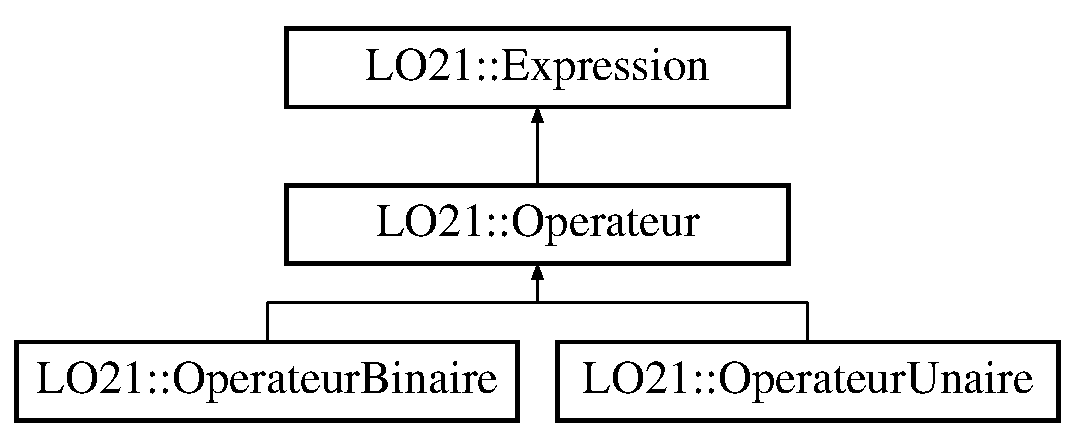
\includegraphics[height=3.000000cm]{class_l_o21_1_1_operateur}
\end{center}
\end{figure}
\subsection*{\-Public \-Member \-Functions}
\begin{DoxyCompactItemize}
\item 
\-Q\-String \hyperlink{class_l_o21_1_1_operateur_a145a86591719c4c74043b05b21722b6e}{to\-String} () const =0
\begin{DoxyCompactList}\small\item\em \-Renvoie une forme textuelle de l'operateur pour affichage. \end{DoxyCompactList}\item 
\-Q\-String \hyperlink{class_l_o21_1_1_operateur_a67c0aa762a71a3dbdb7da4bd8c2ec91d}{get\-Operator} () const 
\begin{DoxyCompactList}\small\item\em \-Retourne le type de l'operateur sous une forme textuelle. \end{DoxyCompactList}\item 
\hypertarget{class_l_o21_1_1_operateur_a93fba96ab13c5c65a426d717fbe6a3ae}{void \hyperlink{class_l_o21_1_1_operateur_a93fba96ab13c5c65a426d717fbe6a3ae}{applique\-Operateur} ()}\label{class_l_o21_1_1_operateur_a93fba96ab13c5c65a426d717fbe6a3ae}

\begin{DoxyCompactList}\small\item\em \-Permet d'appeler la fonction correspondant a un operateur. \end{DoxyCompactList}\item 
\hypertarget{class_l_o21_1_1_operateur_ad82cb92a05c6a0479f05369c5a33121b}{void \hyperlink{class_l_o21_1_1_operateur_ad82cb92a05c6a0479f05369c5a33121b}{\-E\-V\-A\-L} ()}\label{class_l_o21_1_1_operateur_ad82cb92a05c6a0479f05369c5a33121b}

\begin{DoxyCompactList}\small\item\em \-Evalue un operateur. \end{DoxyCompactList}\item 
\-Q\-String \& \hyperlink{class_l_o21_1_1_operateur_a8104fb7f3d740dde10c2e7c4bb2ba660}{afficher} ()
\begin{DoxyCompactList}\small\item\em \-Sert a l'affichage de l'operateur. \end{DoxyCompactList}\item 
\hyperlink{class_l_o21_1_1_operateur}{\-Operateur} $\ast$ \hyperlink{class_l_o21_1_1_operateur_aabf23ebda8447811b12db2f2e174b9d1}{clone} () const 
\begin{DoxyCompactList}\small\item\em \-Permet de dupliquer un objet \hyperlink{class_l_o21_1_1_operateur}{\-Operateur}. \end{DoxyCompactList}\end{DoxyCompactItemize}
\subsection*{\-Protected \-Attributes}
\begin{DoxyCompactItemize}
\item 
\hypertarget{class_l_o21_1_1_operateur_a137931be758a4f6e199d599301bc6b36}{\hyperlink{namespace_l_o21_ad50ab07e90eb3964a086c2f7d95fb8d2}{enum\-Operateurs} {\bfseries \-\_\-operateur}}\label{class_l_o21_1_1_operateur_a137931be758a4f6e199d599301bc6b36}

\end{DoxyCompactItemize}


\subsection{\-Detailed \-Description}
\-Classe permettant de gerer les differents types d'operateurs. 

\subsection{\-Member \-Function \-Documentation}
\hypertarget{class_l_o21_1_1_operateur_a8104fb7f3d740dde10c2e7c4bb2ba660}{\index{\-L\-O21\-::\-Operateur@{\-L\-O21\-::\-Operateur}!afficher@{afficher}}
\index{afficher@{afficher}!LO21::Operateur@{\-L\-O21\-::\-Operateur}}
\subsubsection[{afficher}]{\setlength{\rightskip}{0pt plus 5cm}\-Q\-String \& {\bf \-L\-O21\-::\-Operateur\-::afficher} (
\begin{DoxyParamCaption}
{}
\end{DoxyParamCaption}
)}}\label{class_l_o21_1_1_operateur_a8104fb7f3d740dde10c2e7c4bb2ba660}


\-Sert a l'affichage de l'operateur. 

\begin{DoxyReturn}{\-Returns}
\-Q\-String\& une reference vers le \-Q\-String contenant l'affichage textuel de l'operateur 
\end{DoxyReturn}
\hypertarget{class_l_o21_1_1_operateur_aabf23ebda8447811b12db2f2e174b9d1}{\index{\-L\-O21\-::\-Operateur@{\-L\-O21\-::\-Operateur}!clone@{clone}}
\index{clone@{clone}!LO21::Operateur@{\-L\-O21\-::\-Operateur}}
\subsubsection[{clone}]{\setlength{\rightskip}{0pt plus 5cm}{\bf \-Operateur} $\ast$ {\bf \-L\-O21\-::\-Operateur\-::clone} (
\begin{DoxyParamCaption}
{}
\end{DoxyParamCaption}
) const\hspace{0.3cm}{\ttfamily  \mbox{[}virtual\mbox{]}}}}\label{class_l_o21_1_1_operateur_aabf23ebda8447811b12db2f2e174b9d1}


\-Permet de dupliquer un objet \hyperlink{class_l_o21_1_1_operateur}{\-Operateur}. 

\begin{DoxyReturn}{\-Returns}
\-Operateur$\ast$ un pointeur vers l'operateur nouvellement cree 
\end{DoxyReturn}


\-Implements \hyperlink{class_l_o21_1_1_expression_ad2c9e5301c976f9a2d40edaff0332715}{\-L\-O21\-::\-Expression}.

\hypertarget{class_l_o21_1_1_operateur_a67c0aa762a71a3dbdb7da4bd8c2ec91d}{\index{\-L\-O21\-::\-Operateur@{\-L\-O21\-::\-Operateur}!get\-Operator@{get\-Operator}}
\index{get\-Operator@{get\-Operator}!LO21::Operateur@{\-L\-O21\-::\-Operateur}}
\subsubsection[{get\-Operator}]{\setlength{\rightskip}{0pt plus 5cm}\-Q\-String {\bf \-L\-O21\-::\-Operateur\-::get\-Operator} (
\begin{DoxyParamCaption}
{}
\end{DoxyParamCaption}
) const\hspace{0.3cm}{\ttfamily  \mbox{[}inline\mbox{]}}}}\label{class_l_o21_1_1_operateur_a67c0aa762a71a3dbdb7da4bd8c2ec91d}


\-Retourne le type de l'operateur sous une forme textuelle. 

\begin{DoxyReturn}{\-Returns}
\-Q\-String qui est le texte de l'operateur 
\end{DoxyReturn}
\hypertarget{class_l_o21_1_1_operateur_a145a86591719c4c74043b05b21722b6e}{\index{\-L\-O21\-::\-Operateur@{\-L\-O21\-::\-Operateur}!to\-String@{to\-String}}
\index{to\-String@{to\-String}!LO21::Operateur@{\-L\-O21\-::\-Operateur}}
\subsubsection[{to\-String}]{\setlength{\rightskip}{0pt plus 5cm}\-Q\-String {\bf \-L\-O21\-::\-Operateur\-::to\-String} (
\begin{DoxyParamCaption}
{}
\end{DoxyParamCaption}
) const\hspace{0.3cm}{\ttfamily  \mbox{[}pure virtual\mbox{]}}}}\label{class_l_o21_1_1_operateur_a145a86591719c4c74043b05b21722b6e}


\-Renvoie une forme textuelle de l'operateur pour affichage. 

\-Le type de l'operateur

\begin{DoxyReturn}{\-Returns}
\-Q\-String contenant le texte correspondant a l'operateur 
\end{DoxyReturn}


\-Implements \hyperlink{class_l_o21_1_1_expression}{\-L\-O21\-::\-Expression}.



\-Implemented in \hyperlink{class_l_o21_1_1_operateur_binaire_a7a25e004beb162f80873002759b4310e}{\-L\-O21\-::\-Operateur\-Binaire}, and \hyperlink{class_l_o21_1_1_operateur_unaire_a5b54c985de0fc559337f914771779185}{\-L\-O21\-::\-Operateur\-Unaire}.



\-The documentation for this class was generated from the following files\-:\begin{DoxyCompactItemize}
\item 
\hyperlink{_operateur_8h}{\-Operateur.\-h}\item 
\-Operateur.\-cpp\end{DoxyCompactItemize}

\hypertarget{class_l_o21_1_1_operateur_binaire}{\section{\-L\-O21\-:\-:\-Operateur\-Binaire \-Class \-Reference}
\label{class_l_o21_1_1_operateur_binaire}\index{\-L\-O21\-::\-Operateur\-Binaire@{\-L\-O21\-::\-Operateur\-Binaire}}
}


\-Classe permettant de gerer les operateurs binaires presents dans une expression.  




{\ttfamily \#include $<$\-Operateur\-Binaire.\-h$>$}

\-Inheritance diagram for \-L\-O21\-:\-:\-Operateur\-Binaire\-:\begin{figure}[H]
\begin{center}
\leavevmode
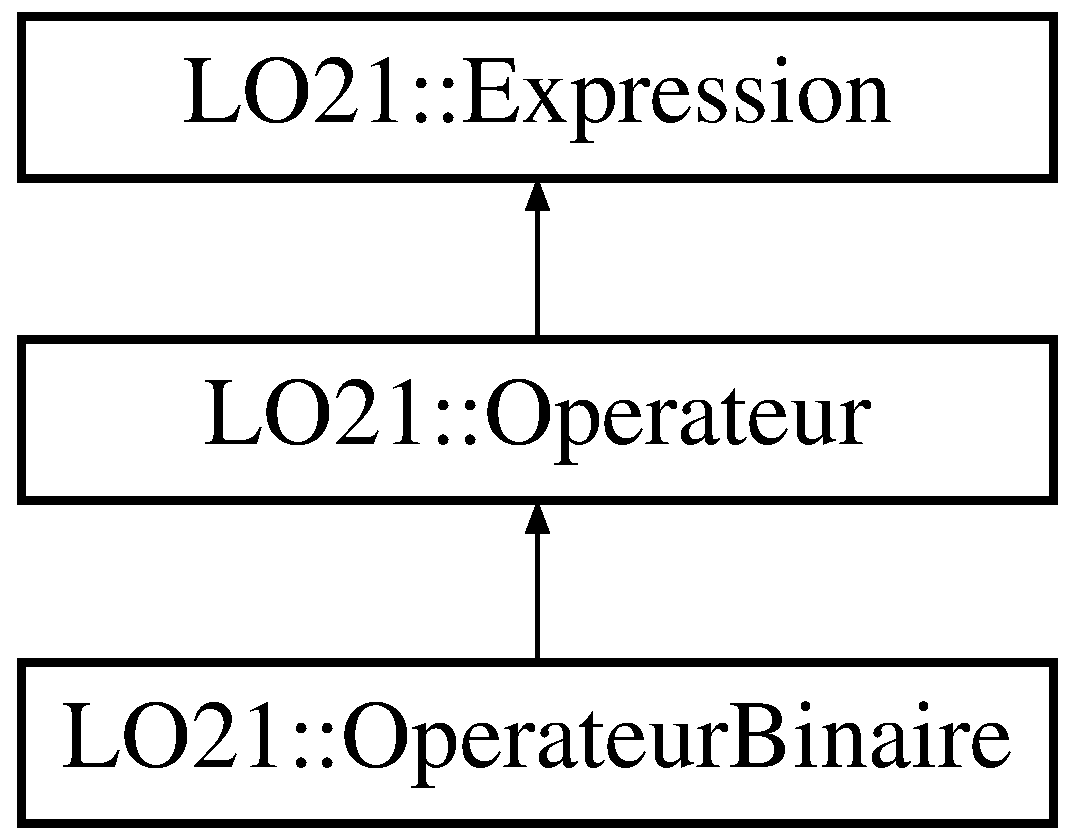
\includegraphics[height=3.000000cm]{class_l_o21_1_1_operateur_binaire}
\end{center}
\end{figure}
\subsection*{\-Public \-Member \-Functions}
\begin{DoxyCompactItemize}
\item 
\hyperlink{class_l_o21_1_1_operateur_binaire_a09e3546e9c5f993e549aedd6b26b3ca5}{\-Operateur\-Binaire} (const \-Q\-String \&op)
\begin{DoxyCompactList}\small\item\em \-Constructeur de la classe \hyperlink{class_l_o21_1_1_operateur_binaire}{\-Operateur\-Binaire}. \end{DoxyCompactList}\item 
\-Q\-String \hyperlink{class_l_o21_1_1_operateur_binaire_a7a25e004beb162f80873002759b4310e}{to\-String} () const 
\begin{DoxyCompactList}\small\item\em \-Permet de donner une forme textuelle a l'operateur. \end{DoxyCompactList}\end{DoxyCompactItemize}


\subsection{\-Detailed \-Description}
\-Classe permettant de gerer les operateurs binaires presents dans une expression. 

\subsection{\-Constructor \& \-Destructor \-Documentation}
\hypertarget{class_l_o21_1_1_operateur_binaire_a09e3546e9c5f993e549aedd6b26b3ca5}{\index{\-L\-O21\-::\-Operateur\-Binaire@{\-L\-O21\-::\-Operateur\-Binaire}!\-Operateur\-Binaire@{\-Operateur\-Binaire}}
\index{\-Operateur\-Binaire@{\-Operateur\-Binaire}!LO21::OperateurBinaire@{\-L\-O21\-::\-Operateur\-Binaire}}
\subsubsection[{\-Operateur\-Binaire}]{\setlength{\rightskip}{0pt plus 5cm}{\bf \-L\-O21\-::\-Operateur\-Binaire\-::\-Operateur\-Binaire} (
\begin{DoxyParamCaption}
\item[{const \-Q\-String \&}]{op}
\end{DoxyParamCaption}
)}}\label{class_l_o21_1_1_operateur_binaire_a09e3546e9c5f993e549aedd6b26b3ca5}


\-Constructeur de la classe \hyperlink{class_l_o21_1_1_operateur_binaire}{\-Operateur\-Binaire}. 


\begin{DoxyParams}{\-Parameters}
{\em op} & le type de l'operateur \\
\hline
\end{DoxyParams}


\subsection{\-Member \-Function \-Documentation}
\hypertarget{class_l_o21_1_1_operateur_binaire_a7a25e004beb162f80873002759b4310e}{\index{\-L\-O21\-::\-Operateur\-Binaire@{\-L\-O21\-::\-Operateur\-Binaire}!to\-String@{to\-String}}
\index{to\-String@{to\-String}!LO21::OperateurBinaire@{\-L\-O21\-::\-Operateur\-Binaire}}
\subsubsection[{to\-String}]{\setlength{\rightskip}{0pt plus 5cm}\-Q\-String {\bf \-L\-O21\-::\-Operateur\-Binaire\-::to\-String} (
\begin{DoxyParamCaption}
{}
\end{DoxyParamCaption}
) const\hspace{0.3cm}{\ttfamily  \mbox{[}virtual\mbox{]}}}}\label{class_l_o21_1_1_operateur_binaire_a7a25e004beb162f80873002759b4310e}


\-Permet de donner une forme textuelle a l'operateur. 

\begin{DoxyReturn}{\-Returns}
\-Q\-String contenant la version textualisee de l'operateur 
\end{DoxyReturn}


\-Implements \hyperlink{class_l_o21_1_1_operateur_a145a86591719c4c74043b05b21722b6e}{\-L\-O21\-::\-Operateur}.



\-The documentation for this class was generated from the following files\-:\begin{DoxyCompactItemize}
\item 
\hyperlink{_operateur_binaire_8h}{\-Operateur\-Binaire.\-h}\item 
\-Operateur\-Binaire.\-cpp\end{DoxyCompactItemize}

\hypertarget{class_l_o21_1_1_operateur_unaire}{\section{\-L\-O21\-:\-:\-Operateur\-Unaire \-Class \-Reference}
\label{class_l_o21_1_1_operateur_unaire}\index{\-L\-O21\-::\-Operateur\-Unaire@{\-L\-O21\-::\-Operateur\-Unaire}}
}


\-Classe permettant de gerer les operateurs unaires presents dans une expression.  




{\ttfamily \#include $<$\-Operateur\-Unaire.\-h$>$}

\-Inheritance diagram for \-L\-O21\-:\-:\-Operateur\-Unaire\-:\begin{figure}[H]
\begin{center}
\leavevmode
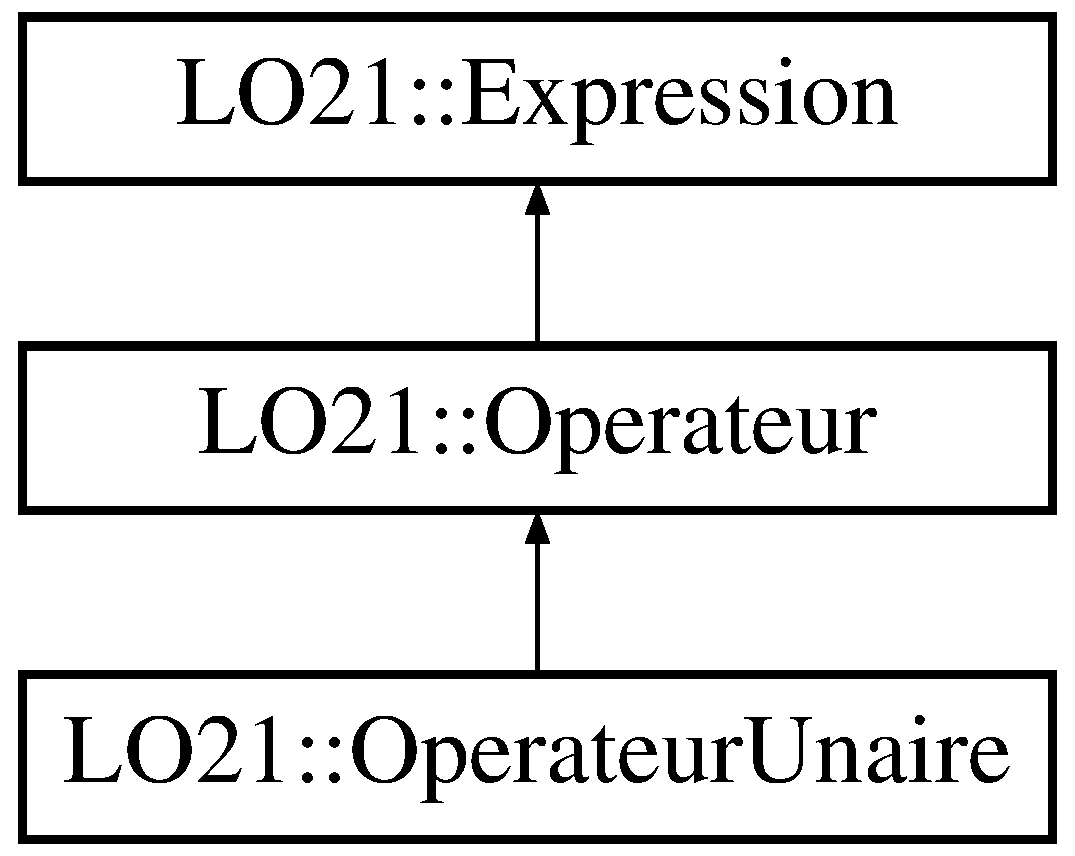
\includegraphics[height=3.000000cm]{class_l_o21_1_1_operateur_unaire}
\end{center}
\end{figure}
\subsection*{\-Public \-Member \-Functions}
\begin{DoxyCompactItemize}
\item 
\hyperlink{class_l_o21_1_1_operateur_unaire_a883e5bfbdfa425834bcf8635bdc95954}{\-Operateur\-Unaire} (const \-Q\-String op)
\begin{DoxyCompactList}\small\item\em \-Constructeur de la classe \hyperlink{class_l_o21_1_1_operateur_unaire}{\-Operateur\-Unaire}. \end{DoxyCompactList}\item 
\-Q\-String \hyperlink{class_l_o21_1_1_operateur_unaire_a5b54c985de0fc559337f914771779185}{to\-String} () const 
\begin{DoxyCompactList}\small\item\em \-Permet de donner une forme textuelle a l'operateur. \end{DoxyCompactList}\end{DoxyCompactItemize}


\subsection{\-Detailed \-Description}
\-Classe permettant de gerer les operateurs unaires presents dans une expression. 

\subsection{\-Constructor \& \-Destructor \-Documentation}
\hypertarget{class_l_o21_1_1_operateur_unaire_a883e5bfbdfa425834bcf8635bdc95954}{\index{\-L\-O21\-::\-Operateur\-Unaire@{\-L\-O21\-::\-Operateur\-Unaire}!\-Operateur\-Unaire@{\-Operateur\-Unaire}}
\index{\-Operateur\-Unaire@{\-Operateur\-Unaire}!LO21::OperateurUnaire@{\-L\-O21\-::\-Operateur\-Unaire}}
\subsubsection[{\-Operateur\-Unaire}]{\setlength{\rightskip}{0pt plus 5cm}{\bf \-L\-O21\-::\-Operateur\-Unaire\-::\-Operateur\-Unaire} (
\begin{DoxyParamCaption}
\item[{const \-Q\-String}]{op}
\end{DoxyParamCaption}
)}}\label{class_l_o21_1_1_operateur_unaire_a883e5bfbdfa425834bcf8635bdc95954}


\-Constructeur de la classe \hyperlink{class_l_o21_1_1_operateur_unaire}{\-Operateur\-Unaire}. 


\begin{DoxyParams}{\-Parameters}
{\em op} & le type d'operateur \\
\hline
\end{DoxyParams}


\subsection{\-Member \-Function \-Documentation}
\hypertarget{class_l_o21_1_1_operateur_unaire_a5b54c985de0fc559337f914771779185}{\index{\-L\-O21\-::\-Operateur\-Unaire@{\-L\-O21\-::\-Operateur\-Unaire}!to\-String@{to\-String}}
\index{to\-String@{to\-String}!LO21::OperateurUnaire@{\-L\-O21\-::\-Operateur\-Unaire}}
\subsubsection[{to\-String}]{\setlength{\rightskip}{0pt plus 5cm}\-Q\-String {\bf \-L\-O21\-::\-Operateur\-Unaire\-::to\-String} (
\begin{DoxyParamCaption}
{}
\end{DoxyParamCaption}
) const\hspace{0.3cm}{\ttfamily  \mbox{[}virtual\mbox{]}}}}\label{class_l_o21_1_1_operateur_unaire_a5b54c985de0fc559337f914771779185}


\-Permet de donner une forme textuelle a l'operateur. 

\begin{DoxyReturn}{\-Returns}
\-Q\-String contenant la version textualisee de l'operateur 
\end{DoxyReturn}


\-Implements \hyperlink{class_l_o21_1_1_operateur_a145a86591719c4c74043b05b21722b6e}{\-L\-O21\-::\-Operateur}.



\-The documentation for this class was generated from the following files\-:\begin{DoxyCompactItemize}
\item 
\hyperlink{_operateur_unaire_8h}{\-Operateur\-Unaire.\-h}\item 
\-Operateur\-Unaire.\-cpp\end{DoxyCompactItemize}

\hypertarget{class_l_o21_1_1_option}{\section{\-L\-O21\-:\-:\-Option \-Class \-Reference}
\label{class_l_o21_1_1_option}\index{\-L\-O21\-::\-Option@{\-L\-O21\-::\-Option}}
}


\-Classe permettant de gerer les options gerees par l'utilisateur, implementant le design pattern \-Singleton.  




{\ttfamily \#include $<$\-Option.\-h$>$}

\subsection*{\-Public \-Member \-Functions}
\begin{DoxyCompactItemize}
\item 
void \hyperlink{class_l_o21_1_1_option_a22b390cfd4b7ac74b656549d0a4b9e5a}{set\-\_\-type\-Div} (\hyperlink{_option_8h_aa88892c4cb734ae333411b4409f27f72}{\-Type\-Div} s)
\begin{DoxyCompactList}\small\item\em \-Modifie le type de constante selectionne par l'utilisateur. \end{DoxyCompactList}\item 
\hypertarget{class_l_o21_1_1_option_a9c7b2191e0dd3daa235a43aafa317126}{void {\bfseries set\-\_\-complexe} (bool b)}\label{class_l_o21_1_1_option_a9c7b2191e0dd3daa235a43aafa317126}

\item 
\hypertarget{class_l_o21_1_1_option_aa5de72b352852815e35d205796f04d77}{void {\bfseries set\-\_\-degre} (bool b)}\label{class_l_o21_1_1_option_aa5de72b352852815e35d205796f04d77}

\item 
\hyperlink{_option_8h_aa88892c4cb734ae333411b4409f27f72}{\-Type\-Div} \hyperlink{class_l_o21_1_1_option_af694fc0bcf5628c360aaddd371f71975}{get\-\_\-type\-Div} () const 
\begin{DoxyCompactList}\small\item\em \-Retourne le type de constante selectionne. \end{DoxyCompactList}\item 
\hypertarget{class_l_o21_1_1_option_abdd291391f98c3cfebb1269d73c991b6}{bool {\bfseries get\-\_\-degre} () const }\label{class_l_o21_1_1_option_abdd291391f98c3cfebb1269d73c991b6}

\item 
\hypertarget{class_l_o21_1_1_option_a85c4404b22e2c62dd0186880a7384efc}{bool {\bfseries get\-\_\-complexe} () const }\label{class_l_o21_1_1_option_a85c4404b22e2c62dd0186880a7384efc}

\item 
\hypertarget{class_l_o21_1_1_option_a905539c6f4739562a34d6f897506a31b}{void \hyperlink{class_l_o21_1_1_option_a905539c6f4739562a34d6f897506a31b}{save\-Options} ()}\label{class_l_o21_1_1_option_a905539c6f4739562a34d6f897506a31b}

\begin{DoxyCompactList}\small\item\em \-Sauvegarde dans un fichier les options selectionnees a la fermeture de la calculatrice. \end{DoxyCompactList}\item 
\hypertarget{class_l_o21_1_1_option_a1ba94278e521d1674622bbdb363b0cb0}{\-Q\-String {\bfseries to\-String} () const }\label{class_l_o21_1_1_option_a1ba94278e521d1674622bbdb363b0cb0}

\end{DoxyCompactItemize}
\subsection*{\-Static \-Public \-Member \-Functions}
\begin{DoxyCompactItemize}
\item 
static \hyperlink{class_l_o21_1_1_option}{\-Option} \& \hyperlink{class_l_o21_1_1_option_a980e676bc500f07a7f9d7c73db24b1d8}{get\-Instance} ()
\begin{DoxyCompactList}\small\item\em \-Recupere l'instance creee de la classe \hyperlink{class_l_o21_1_1_option}{\-Option}, si celle-\/ci n'existe pas, la cree. \end{DoxyCompactList}\item 
\hypertarget{class_l_o21_1_1_option_a343e58ff25fc13b82d1775f08a8add4d}{static void \hyperlink{class_l_o21_1_1_option_a343e58ff25fc13b82d1775f08a8add4d}{libere\-Instance} ()}\label{class_l_o21_1_1_option_a343e58ff25fc13b82d1775f08a8add4d}

\begin{DoxyCompactList}\small\item\em \-Demande la destruction de la classe \hyperlink{class_l_o21_1_1_option}{\-Option}. \end{DoxyCompactList}\end{DoxyCompactItemize}


\subsection{\-Detailed \-Description}
\-Classe permettant de gerer les options gerees par l'utilisateur, implementant le design pattern \-Singleton. 

\subsection{\-Member \-Function \-Documentation}
\hypertarget{class_l_o21_1_1_option_af694fc0bcf5628c360aaddd371f71975}{\index{\-L\-O21\-::\-Option@{\-L\-O21\-::\-Option}!get\-\_\-type\-Div@{get\-\_\-type\-Div}}
\index{get\-\_\-type\-Div@{get\-\_\-type\-Div}!LO21::Option@{\-L\-O21\-::\-Option}}
\subsubsection[{get\-\_\-type\-Div}]{\setlength{\rightskip}{0pt plus 5cm}{\bf \-Type\-Div} {\bf \-L\-O21\-::\-Option\-::get\-\_\-type\-Div} (
\begin{DoxyParamCaption}
{}
\end{DoxyParamCaption}
) const\hspace{0.3cm}{\ttfamily  \mbox{[}inline\mbox{]}}}}\label{class_l_o21_1_1_option_af694fc0bcf5628c360aaddd371f71975}


\-Retourne le type de constante selectionne. 

\begin{DoxyReturn}{\-Returns}
\-Type\-Div le type de constante 
\end{DoxyReturn}
\hypertarget{class_l_o21_1_1_option_a980e676bc500f07a7f9d7c73db24b1d8}{\index{\-L\-O21\-::\-Option@{\-L\-O21\-::\-Option}!get\-Instance@{get\-Instance}}
\index{get\-Instance@{get\-Instance}!LO21::Option@{\-L\-O21\-::\-Option}}
\subsubsection[{get\-Instance}]{\setlength{\rightskip}{0pt plus 5cm}static {\bf \-Option} \& {\bf \-L\-O21\-::\-Option\-::get\-Instance} (
\begin{DoxyParamCaption}
{}
\end{DoxyParamCaption}
)\hspace{0.3cm}{\ttfamily  \mbox{[}static\mbox{]}}}}\label{class_l_o21_1_1_option_a980e676bc500f07a7f9d7c73db24b1d8}


\-Recupere l'instance creee de la classe \hyperlink{class_l_o21_1_1_option}{\-Option}, si celle-\/ci n'existe pas, la cree. 

\begin{DoxyReturn}{\-Returns}
\hyperlink{class_l_o21_1_1_option}{\-Option}\& une reference vers l'instance de la classe \hyperlink{class_l_o21_1_1_option}{\-Option} 
\end{DoxyReturn}
\hypertarget{class_l_o21_1_1_option_a22b390cfd4b7ac74b656549d0a4b9e5a}{\index{\-L\-O21\-::\-Option@{\-L\-O21\-::\-Option}!set\-\_\-type\-Div@{set\-\_\-type\-Div}}
\index{set\-\_\-type\-Div@{set\-\_\-type\-Div}!LO21::Option@{\-L\-O21\-::\-Option}}
\subsubsection[{set\-\_\-type\-Div}]{\setlength{\rightskip}{0pt plus 5cm}void {\bf \-L\-O21\-::\-Option\-::set\-\_\-type\-Div} (
\begin{DoxyParamCaption}
\item[{{\bf \-Type\-Div}}]{s}
\end{DoxyParamCaption}
)}}\label{class_l_o21_1_1_option_a22b390cfd4b7ac74b656549d0a4b9e5a}


\-Modifie le type de constante selectionne par l'utilisateur. 


\begin{DoxyParams}{\-Parameters}
{\em s} & le type de constante selectionne \\
\hline
\end{DoxyParams}


\-The documentation for this class was generated from the following files\-:\begin{DoxyCompactItemize}
\item 
\hyperlink{_option_8h}{\-Option.\-h}\item 
\-Option.\-cpp\end{DoxyCompactItemize}

\hypertarget{class_l_o21_1_1_pile}{\section{\-L\-O21\-:\-:\-Pile \-Class \-Reference}
\label{class_l_o21_1_1_pile}\index{\-L\-O21\-::\-Pile@{\-L\-O21\-::\-Pile}}
}


\-Classe stockant et manipulant les \-Expressions pour calcul.  




{\ttfamily \#include $<$\-Pile.\-h$>$}

\subsection*{\-Classes}
\begin{DoxyCompactItemize}
\item 
class \hyperlink{class_l_o21_1_1_pile_1_1_memento}{\-Memento}
\begin{DoxyCompactList}\small\item\em \-Classe permettant de gerer divers etats d'un meme objet. \end{DoxyCompactList}\end{DoxyCompactItemize}
\subsection*{\-Public \-Member \-Functions}
\begin{DoxyCompactItemize}
\item 
\hyperlink{class_l_o21_1_1_pile_aace652ebfd029827297fdedc294288f2}{\-Pile} ()
\begin{DoxyCompactList}\small\item\em \-Constructeur par defaut de la classe \hyperlink{class_l_o21_1_1_pile}{\-Pile}. \end{DoxyCompactList}\item 
void \hyperlink{class_l_o21_1_1_pile_a9d322532282fb52a1bdd0d870c77f381}{\-S\-W\-A\-P} (int x, int y)
\begin{DoxyCompactList}\small\item\em \-Permet d'echanger la place de deux elements dans la pile. \end{DoxyCompactList}\item 
\hypertarget{class_l_o21_1_1_pile_a921e68479ce5ac4e609903da41b0a4e6}{void \hyperlink{class_l_o21_1_1_pile_a921e68479ce5ac4e609903da41b0a4e6}{\-S\-U\-M} (int n)}\label{class_l_o21_1_1_pile_a921e68479ce5ac4e609903da41b0a4e6}

\begin{DoxyCompactList}\small\item\em \-Calculer la somme des n premiers elements de la pile. \end{DoxyCompactList}\item 
\hypertarget{class_l_o21_1_1_pile_adea674770f7f3957c0ba6368ca61e302}{void \hyperlink{class_l_o21_1_1_pile_adea674770f7f3957c0ba6368ca61e302}{\-M\-E\-A\-N} (int n)}\label{class_l_o21_1_1_pile_adea674770f7f3957c0ba6368ca61e302}

\begin{DoxyCompactList}\small\item\em \-Calcule la moyenne des n premiers elements de la pile. \end{DoxyCompactList}\item 
\hypertarget{class_l_o21_1_1_pile_aac45f9bf192afd3738c981ef1a934bc0}{void \hyperlink{class_l_o21_1_1_pile_aac45f9bf192afd3738c981ef1a934bc0}{\-C\-L\-E\-A\-R} ()}\label{class_l_o21_1_1_pile_aac45f9bf192afd3738c981ef1a934bc0}

\begin{DoxyCompactList}\small\item\em \-Efface toutes les \-Expressions presentes dans la pile. \end{DoxyCompactList}\item 
\hypertarget{class_l_o21_1_1_pile_a787e1174fff99237d055fb2818fa3996}{void \hyperlink{class_l_o21_1_1_pile_a787e1174fff99237d055fb2818fa3996}{\-D\-U\-P} ()}\label{class_l_o21_1_1_pile_a787e1174fff99237d055fb2818fa3996}

\begin{DoxyCompactList}\small\item\em \-Duplique l'element au sommet de la pile. \end{DoxyCompactList}\item 
\hypertarget{class_l_o21_1_1_pile_a3a66cfb9e89b7b8ec0e6b75958183633}{void \hyperlink{class_l_o21_1_1_pile_a3a66cfb9e89b7b8ec0e6b75958183633}{\-D\-R\-O\-P} ()}\label{class_l_o21_1_1_pile_a3a66cfb9e89b7b8ec0e6b75958183633}

\begin{DoxyCompactList}\small\item\em \-Ote l'element au sommet de la pile. \end{DoxyCompactList}\item 
\hypertarget{class_l_o21_1_1_pile_a6eeceaf747f06fcb798e19e4fbb9b5ea}{void \hyperlink{class_l_o21_1_1_pile_a6eeceaf747f06fcb798e19e4fbb9b5ea}{sauvegarder} ()}\label{class_l_o21_1_1_pile_a6eeceaf747f06fcb798e19e4fbb9b5ea}

\begin{DoxyCompactList}\small\item\em \-Sauvegarde l'etat actuel de la pile. \end{DoxyCompactList}\item 
\hypertarget{class_l_o21_1_1_pile_aaf626065c4b7e5ef54b1a7663111f882}{void \hyperlink{class_l_o21_1_1_pile_aaf626065c4b7e5ef54b1a7663111f882}{charger} ()}\label{class_l_o21_1_1_pile_aaf626065c4b7e5ef54b1a7663111f882}

\begin{DoxyCompactList}\small\item\em \-Charge un etat donne de la pile. \end{DoxyCompactList}\item 
\hyperlink{class_l_o21_1_1_pile}{\-Pile} $\ast$ \hyperlink{class_l_o21_1_1_pile_a6acd2bf5bc8ea9cff26b8a301d12bc00}{clone} () const 
\begin{DoxyCompactList}\small\item\em \-Duplique la pile actuellement utilisee. \end{DoxyCompactList}\item 
\hypertarget{class_l_o21_1_1_pile_ab419ee4250785f1a19572ab5815915cf}{void \hyperlink{class_l_o21_1_1_pile_ab419ee4250785f1a19572ab5815915cf}{afficher\-Pile\-Courante} () const }\label{class_l_o21_1_1_pile_ab419ee4250785f1a19572ab5815915cf}

\begin{DoxyCompactList}\small\item\em \-Affiche les elements presents dans la pile. \end{DoxyCompactList}\item 
\hypertarget{class_l_o21_1_1_pile_a3dbaa1a110fa80d14339df8aed0d9eac}{void \hyperlink{class_l_o21_1_1_pile_a3dbaa1a110fa80d14339df8aed0d9eac}{afficher\-Pile\-Memoire} () const }\label{class_l_o21_1_1_pile_a3dbaa1a110fa80d14339df8aed0d9eac}

\begin{DoxyCompactList}\small\item\em \-Affiche les elements presents dans la pile etant sauvegardee en memoire. \end{DoxyCompactList}\item 
\hyperlink{class_l_o21_1_1_pile_1_1_memento}{\-Memento} $\ast$ \hyperlink{class_l_o21_1_1_pile_aee1e662b5a27fcff0862607e4311d6a8}{sauver\-Dans\-Memento} ()
\begin{DoxyCompactList}\small\item\em \-Permet de sauver l'etat de la pile actuelle. \end{DoxyCompactList}\item 
void \hyperlink{class_l_o21_1_1_pile_a980fa91fee3691e57954dc8a5d4420ce}{restaurer\-Depuis\-Memento} (const \hyperlink{class_l_o21_1_1_pile_1_1_memento}{\-Memento} $\ast$m)
\begin{DoxyCompactList}\small\item\em \-Permet de restaurer la pile a un etat anterieur sauve dans l'objet \hyperlink{class_l_o21_1_1_pile_1_1_memento}{\-Memento}. \end{DoxyCompactList}\item 
\hyperlink{class_l_o21_1_1_pile}{\-Pile} $\ast$ \hyperlink{class_l_o21_1_1_pile_ab7e49a045c7f01c8959f41b1c7af6f60}{get\-\_\-etat} () const 
\begin{DoxyCompactList}\small\item\em \-Retourne l'etat actuel de la pile. \end{DoxyCompactList}\end{DoxyCompactItemize}


\subsection{\-Detailed \-Description}
\-Classe stockant et manipulant les \-Expressions pour calcul. 

\subsection{\-Constructor \& \-Destructor \-Documentation}
\hypertarget{class_l_o21_1_1_pile_aace652ebfd029827297fdedc294288f2}{\index{\-L\-O21\-::\-Pile@{\-L\-O21\-::\-Pile}!\-Pile@{\-Pile}}
\index{\-Pile@{\-Pile}!LO21::Pile@{\-L\-O21\-::\-Pile}}
\subsubsection[{\-Pile}]{\setlength{\rightskip}{0pt plus 5cm}{\bf \-L\-O21\-::\-Pile\-::\-Pile} (
\begin{DoxyParamCaption}
{}
\end{DoxyParamCaption}
)\hspace{0.3cm}{\ttfamily  \mbox{[}inline\mbox{]}}}}\label{class_l_o21_1_1_pile_aace652ebfd029827297fdedc294288f2}


\-Constructeur par defaut de la classe \hyperlink{class_l_o21_1_1_pile}{\-Pile}. 

\-La pile affichee 

\subsection{\-Member \-Function \-Documentation}
\hypertarget{class_l_o21_1_1_pile_a6acd2bf5bc8ea9cff26b8a301d12bc00}{\index{\-L\-O21\-::\-Pile@{\-L\-O21\-::\-Pile}!clone@{clone}}
\index{clone@{clone}!LO21::Pile@{\-L\-O21\-::\-Pile}}
\subsubsection[{clone}]{\setlength{\rightskip}{0pt plus 5cm}{\bf \-Pile} $\ast$ {\bf \-L\-O21\-::\-Pile\-::clone} (
\begin{DoxyParamCaption}
{}
\end{DoxyParamCaption}
) const}}\label{class_l_o21_1_1_pile_a6acd2bf5bc8ea9cff26b8a301d12bc00}


\-Duplique la pile actuellement utilisee. 

\begin{DoxyReturn}{\-Returns}
\-Pile$\ast$ un pointeur vers la pile creee par la pile appelante 
\end{DoxyReturn}
\hypertarget{class_l_o21_1_1_pile_ab7e49a045c7f01c8959f41b1c7af6f60}{\index{\-L\-O21\-::\-Pile@{\-L\-O21\-::\-Pile}!get\-\_\-etat@{get\-\_\-etat}}
\index{get\-\_\-etat@{get\-\_\-etat}!LO21::Pile@{\-L\-O21\-::\-Pile}}
\subsubsection[{get\-\_\-etat}]{\setlength{\rightskip}{0pt plus 5cm}{\bf \-Pile} $\ast$ {\bf \-L\-O21\-::\-Pile\-::get\-\_\-etat} (
\begin{DoxyParamCaption}
{}
\end{DoxyParamCaption}
) const}}\label{class_l_o21_1_1_pile_ab7e49a045c7f01c8959f41b1c7af6f60}


\-Retourne l'etat actuel de la pile. 

\begin{DoxyReturn}{\-Returns}
\-Pile$\ast$ pointeur vers la pile actuelle 
\end{DoxyReturn}
\hypertarget{class_l_o21_1_1_pile_a980fa91fee3691e57954dc8a5d4420ce}{\index{\-L\-O21\-::\-Pile@{\-L\-O21\-::\-Pile}!restaurer\-Depuis\-Memento@{restaurer\-Depuis\-Memento}}
\index{restaurer\-Depuis\-Memento@{restaurer\-Depuis\-Memento}!LO21::Pile@{\-L\-O21\-::\-Pile}}
\subsubsection[{restaurer\-Depuis\-Memento}]{\setlength{\rightskip}{0pt plus 5cm}void {\bf \-L\-O21\-::\-Pile\-::restaurer\-Depuis\-Memento} (
\begin{DoxyParamCaption}
\item[{const {\bf \-Memento} $\ast$}]{m}
\end{DoxyParamCaption}
)}}\label{class_l_o21_1_1_pile_a980fa91fee3691e57954dc8a5d4420ce}


\-Permet de restaurer la pile a un etat anterieur sauve dans l'objet \hyperlink{class_l_o21_1_1_pile_1_1_memento}{\-Memento}. 


\begin{DoxyParams}{\-Parameters}
{\em m} & pointeur vers l'objet \hyperlink{class_l_o21_1_1_pile_1_1_memento}{\-Memento} contenant l'etat a restaurer \\
\hline
\end{DoxyParams}
\hypertarget{class_l_o21_1_1_pile_aee1e662b5a27fcff0862607e4311d6a8}{\index{\-L\-O21\-::\-Pile@{\-L\-O21\-::\-Pile}!sauver\-Dans\-Memento@{sauver\-Dans\-Memento}}
\index{sauver\-Dans\-Memento@{sauver\-Dans\-Memento}!LO21::Pile@{\-L\-O21\-::\-Pile}}
\subsubsection[{sauver\-Dans\-Memento}]{\setlength{\rightskip}{0pt plus 5cm}{\bf \-Memento} $\ast$ {\bf \-L\-O21\-::\-Pile\-::sauver\-Dans\-Memento} (
\begin{DoxyParamCaption}
{}
\end{DoxyParamCaption}
)}}\label{class_l_o21_1_1_pile_aee1e662b5a27fcff0862607e4311d6a8}


\-Permet de sauver l'etat de la pile actuelle. 

\begin{DoxyReturn}{\-Returns}
\-Memento$\ast$ pile vers la structure permettant de sauvegarder l'etaat 
\end{DoxyReturn}
\hypertarget{class_l_o21_1_1_pile_a9d322532282fb52a1bdd0d870c77f381}{\index{\-L\-O21\-::\-Pile@{\-L\-O21\-::\-Pile}!\-S\-W\-A\-P@{\-S\-W\-A\-P}}
\index{\-S\-W\-A\-P@{\-S\-W\-A\-P}!LO21::Pile@{\-L\-O21\-::\-Pile}}
\subsubsection[{\-S\-W\-A\-P}]{\setlength{\rightskip}{0pt plus 5cm}void {\bf \-L\-O21\-::\-Pile\-::\-S\-W\-A\-P} (
\begin{DoxyParamCaption}
\item[{int}]{x, }
\item[{int}]{y}
\end{DoxyParamCaption}
)}}\label{class_l_o21_1_1_pile_a9d322532282fb52a1bdd0d870c77f381}


\-Permet d'echanger la place de deux elements dans la pile. 


\begin{DoxyParams}{\-Parameters}
{\em x} & l'indice du premier element a echanger \\
\hline
{\em y} & l'indice du deuxieme element a echanger \\
\hline
\end{DoxyParams}


\-The documentation for this class was generated from the following files\-:\begin{DoxyCompactItemize}
\item 
\hyperlink{_pile_8h}{\-Pile.\-h}\item 
\-Pile.\-cpp\end{DoxyCompactItemize}

\hypertarget{class_l_o21_1_1_rationnel}{\section{\-L\-O21\-:\-:\-Rationnel \-Class \-Reference}
\label{class_l_o21_1_1_rationnel}\index{\-L\-O21\-::\-Rationnel@{\-L\-O21\-::\-Rationnel}}
}


\-Classe permettant de gerer les nombres rationnels.  




{\ttfamily \#include $<$\-Rationnel.\-h$>$}

\-Inheritance diagram for \-L\-O21\-:\-:\-Rationnel\-:\begin{figure}[H]
\begin{center}
\leavevmode
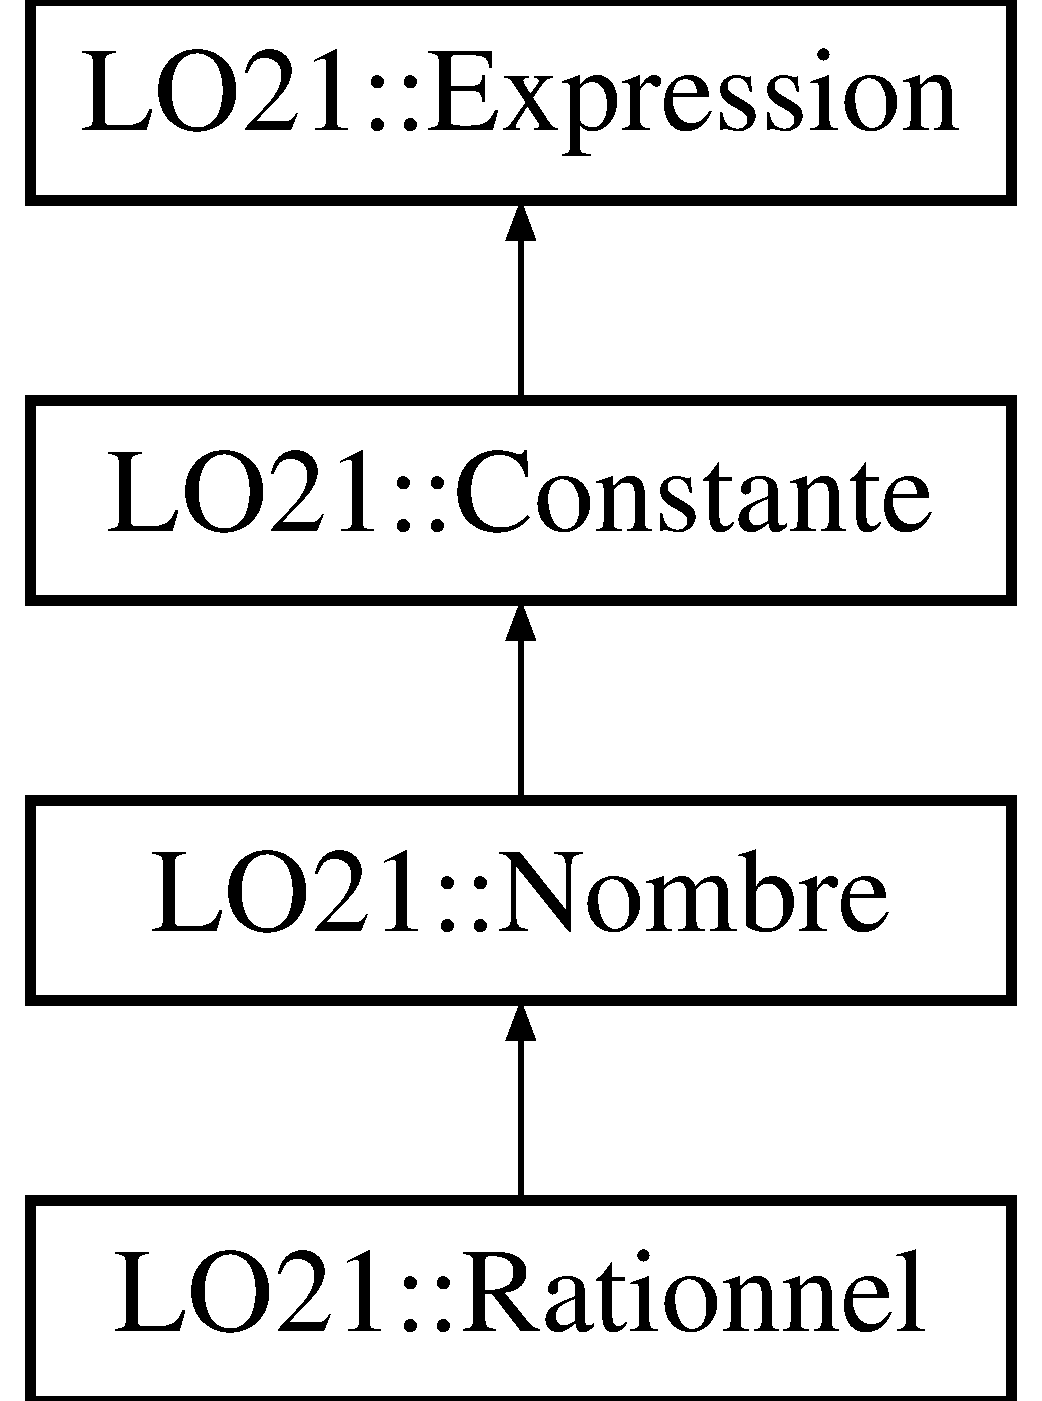
\includegraphics[height=4.000000cm]{class_l_o21_1_1_rationnel}
\end{center}
\end{figure}
\subsection*{\-Public \-Member \-Functions}
\begin{DoxyCompactItemize}
\item 
\hyperlink{class_l_o21_1_1_constante}{\-Constante} \& \hyperlink{class_l_o21_1_1_rationnel_a67e3dea6269482abdf3101e16e53c769}{addition} (const \hyperlink{class_l_o21_1_1_constante}{\-Constante} \&nb) const 
\begin{DoxyCompactList}\small\item\em \-Gere l'addition entre un rationnel et une constante quelle qu'elle soit. \end{DoxyCompactList}\item 
\hyperlink{class_l_o21_1_1_constante}{\-Constante} \& \hyperlink{class_l_o21_1_1_rationnel_a3e0d87746663be866be81543d552b6a1}{soustraction} (const \hyperlink{class_l_o21_1_1_constante}{\-Constante} \&nb) const 
\begin{DoxyCompactList}\small\item\em \-Gere la soustraction entre un rationnel et une constante quelle qu'elle soit. \end{DoxyCompactList}\item 
\hyperlink{class_l_o21_1_1_constante}{\-Constante} \& \hyperlink{class_l_o21_1_1_rationnel_ad59a24eab43b40d59e639078a9a9d638}{multiplication} (const \hyperlink{class_l_o21_1_1_constante}{\-Constante} \&nb) const 
\begin{DoxyCompactList}\small\item\em \-Gere la multiplication entre un rationnel et une constante quelle qu'elle soit. \end{DoxyCompactList}\item 
\hyperlink{class_l_o21_1_1_constante}{\-Constante} \& \hyperlink{class_l_o21_1_1_rationnel_abc26382a7434c12b941e8c68547985c4}{division} (const \hyperlink{class_l_o21_1_1_constante}{\-Constante} \&nb) const 
\begin{DoxyCompactList}\small\item\em \-Gere la division entre deux constantes quelles qu'elles soient. \end{DoxyCompactList}\item 
\-Q\-String \hyperlink{class_l_o21_1_1_rationnel_a2a7494242bcf30b5163e63133960323b}{to\-String} () const 
\begin{DoxyCompactList}\small\item\em \-Permet l'affichage textualise d'un rationnel. \end{DoxyCompactList}\item 
\hypertarget{class_l_o21_1_1_rationnel_a0ff5f18be13068386dc0c3236835593b}{void \hyperlink{class_l_o21_1_1_rationnel_a0ff5f18be13068386dc0c3236835593b}{simplifier} ()}\label{class_l_o21_1_1_rationnel_a0ff5f18be13068386dc0c3236835593b}

\begin{DoxyCompactList}\small\item\em \-Simplifie la fonction. \end{DoxyCompactList}\item 
\hyperlink{class_l_o21_1_1_reel}{\-Reel} \& \hyperlink{class_l_o21_1_1_rationnel_ae99865dd4a35cd635e2918c120cc71cb}{to\-Reel} () const 
\begin{DoxyCompactList}\small\item\em \-Transforme un rationnel en reel. \end{DoxyCompactList}\item 
\hyperlink{class_l_o21_1_1_entier}{\-Entier} \& \hyperlink{class_l_o21_1_1_rationnel_acc531bade32af7c76f84b5ab150c0408}{to\-Entier} () const 
\begin{DoxyCompactList}\small\item\em \-Transforme un rationnel en entier. \end{DoxyCompactList}\item 
\hyperlink{class_l_o21_1_1_complexe}{\-Complexe} \& \hyperlink{class_l_o21_1_1_rationnel_af868bb26a890f1a8eff86feb2c2ca866}{to\-Complexe} () const 
\begin{DoxyCompactList}\small\item\em \-Transforme un rationnel en complexe. \end{DoxyCompactList}\item 
const \hyperlink{class_l_o21_1_1_entier}{\-Entier} \& \hyperlink{class_l_o21_1_1_rationnel_a5442e6750fee7814eec132283965eef7}{get\-\_\-n} () const 
\begin{DoxyCompactList}\small\item\em \-Retourne le numerateur du rationnel. \end{DoxyCompactList}\item 
const \hyperlink{class_l_o21_1_1_entier}{\-Entier} \& \hyperlink{class_l_o21_1_1_rationnel_abffbfed0e03c7b0a560534cdeccfda89}{get\-\_\-d} () const 
\begin{DoxyCompactList}\small\item\em \-Retourne le denominateur du rationnel. \end{DoxyCompactList}\item 
\hyperlink{class_l_o21_1_1_rationnel_a0fb60948285eb5e4bdde460b0ca52ac9}{\-Rationnel} (const \hyperlink{class_l_o21_1_1_entier}{\-Entier} \&x, const \hyperlink{class_l_o21_1_1_entier}{\-Entier} \&y)
\begin{DoxyCompactList}\small\item\em \-Constructeur de la classe \hyperlink{class_l_o21_1_1_rationnel}{\-Rationnel}. \end{DoxyCompactList}\item 
\hyperlink{class_l_o21_1_1_rationnel_ab65f604ee61543f81ad3192b00475d0c}{\-Rationnel} (unsigned int x=0, unsigned int y=1)
\begin{DoxyCompactList}\small\item\em \-Constructeur de la classe \hyperlink{class_l_o21_1_1_rationnel}{\-Rationnel}. \end{DoxyCompactList}\item 
\hyperlink{class_l_o21_1_1_rationnel}{\-Rationnel} $\ast$ \hyperlink{class_l_o21_1_1_rationnel_aab7de5f24ff5fa9f5d250e8b096ceb34}{clone} () const 
\begin{DoxyCompactList}\small\item\em \-Cree une copie de l'objet appelant. \end{DoxyCompactList}\end{DoxyCompactItemize}


\subsection{\-Detailed \-Description}
\-Classe permettant de gerer les nombres rationnels. 

\subsection{\-Constructor \& \-Destructor \-Documentation}
\hypertarget{class_l_o21_1_1_rationnel_a0fb60948285eb5e4bdde460b0ca52ac9}{\index{\-L\-O21\-::\-Rationnel@{\-L\-O21\-::\-Rationnel}!\-Rationnel@{\-Rationnel}}
\index{\-Rationnel@{\-Rationnel}!LO21::Rationnel@{\-L\-O21\-::\-Rationnel}}
\subsubsection[{\-Rationnel}]{\setlength{\rightskip}{0pt plus 5cm}{\bf \-L\-O21\-::\-Rationnel\-::\-Rationnel} (
\begin{DoxyParamCaption}
\item[{const {\bf \-Entier} \&}]{x, }
\item[{const {\bf \-Entier} \&}]{y}
\end{DoxyParamCaption}
)\hspace{0.3cm}{\ttfamily  \mbox{[}inline\mbox{]}}}}\label{class_l_o21_1_1_rationnel_a0fb60948285eb5e4bdde460b0ca52ac9}


\-Constructeur de la classe \hyperlink{class_l_o21_1_1_rationnel}{\-Rationnel}. 


\begin{DoxyParams}{\-Parameters}
{\em x} & une reference vers un objet \hyperlink{class_l_o21_1_1_entier}{\-Entier} representant le numerateur du rationnel \\
\hline
{\em y} & une reference vers un objet \hyperlink{class_l_o21_1_1_entier}{\-Entier} representant le denominateur du rationnel \\
\hline
\end{DoxyParams}
\hypertarget{class_l_o21_1_1_rationnel_ab65f604ee61543f81ad3192b00475d0c}{\index{\-L\-O21\-::\-Rationnel@{\-L\-O21\-::\-Rationnel}!\-Rationnel@{\-Rationnel}}
\index{\-Rationnel@{\-Rationnel}!LO21::Rationnel@{\-L\-O21\-::\-Rationnel}}
\subsubsection[{\-Rationnel}]{\setlength{\rightskip}{0pt plus 5cm}{\bf \-L\-O21\-::\-Rationnel\-::\-Rationnel} (
\begin{DoxyParamCaption}
\item[{unsigned int}]{x = {\ttfamily 0}, }
\item[{unsigned int}]{y = {\ttfamily 1}}
\end{DoxyParamCaption}
)\hspace{0.3cm}{\ttfamily  \mbox{[}inline\mbox{]}}}}\label{class_l_o21_1_1_rationnel_ab65f604ee61543f81ad3192b00475d0c}


\-Constructeur de la classe \hyperlink{class_l_o21_1_1_rationnel}{\-Rationnel}. 


\begin{DoxyParams}{\-Parameters}
{\em x} & un entier representant le numerateur du rationnel \\
\hline
{\em y} & un entier representant le denominateur du rationnel \\
\hline
\end{DoxyParams}


\subsection{\-Member \-Function \-Documentation}
\hypertarget{class_l_o21_1_1_rationnel_a67e3dea6269482abdf3101e16e53c769}{\index{\-L\-O21\-::\-Rationnel@{\-L\-O21\-::\-Rationnel}!addition@{addition}}
\index{addition@{addition}!LO21::Rationnel@{\-L\-O21\-::\-Rationnel}}
\subsubsection[{addition}]{\setlength{\rightskip}{0pt plus 5cm}{\bf \-Constante} \& {\bf \-L\-O21\-::\-Rationnel\-::addition} (
\begin{DoxyParamCaption}
\item[{const {\bf \-Constante} \&}]{nb}
\end{DoxyParamCaption}
) const\hspace{0.3cm}{\ttfamily  \mbox{[}virtual\mbox{]}}}}\label{class_l_o21_1_1_rationnel_a67e3dea6269482abdf3101e16e53c769}


\-Gere l'addition entre un rationnel et une constante quelle qu'elle soit. 

\-Le denominateur de la fraction


\begin{DoxyParams}{\-Parameters}
{\em nb} & une reference vers une constante \\
\hline
\end{DoxyParams}
\begin{DoxyReturn}{\-Returns}
\hyperlink{class_l_o21_1_1_constante}{\-Constante}\& une reference vers la constante creee a partir du resultat 
\end{DoxyReturn}


\-Implements \hyperlink{class_l_o21_1_1_nombre_a75c7a5c063ed122f7ba004e09f1f6621}{\-L\-O21\-::\-Nombre}.

\hypertarget{class_l_o21_1_1_rationnel_aab7de5f24ff5fa9f5d250e8b096ceb34}{\index{\-L\-O21\-::\-Rationnel@{\-L\-O21\-::\-Rationnel}!clone@{clone}}
\index{clone@{clone}!LO21::Rationnel@{\-L\-O21\-::\-Rationnel}}
\subsubsection[{clone}]{\setlength{\rightskip}{0pt plus 5cm}{\bf \-Rationnel} $\ast$ {\bf \-L\-O21\-::\-Rationnel\-::clone} (
\begin{DoxyParamCaption}
{}
\end{DoxyParamCaption}
) const\hspace{0.3cm}{\ttfamily  \mbox{[}virtual\mbox{]}}}}\label{class_l_o21_1_1_rationnel_aab7de5f24ff5fa9f5d250e8b096ceb34}


\-Cree une copie de l'objet appelant. 

\begin{DoxyReturn}{\-Returns}
\-Rationnel$\ast$ un pointeur vers le rationnel issu de la recopie de l'objet 
\end{DoxyReturn}


\-Implements \hyperlink{class_l_o21_1_1_nombre_aea071e3bcebfdc9337eaea8515e248c9}{\-L\-O21\-::\-Nombre}.

\hypertarget{class_l_o21_1_1_rationnel_abc26382a7434c12b941e8c68547985c4}{\index{\-L\-O21\-::\-Rationnel@{\-L\-O21\-::\-Rationnel}!division@{division}}
\index{division@{division}!LO21::Rationnel@{\-L\-O21\-::\-Rationnel}}
\subsubsection[{division}]{\setlength{\rightskip}{0pt plus 5cm}{\bf \-L\-O21\-::\-Constante} \& {\bf \-L\-O21\-::\-Rationnel\-::division} (
\begin{DoxyParamCaption}
\item[{const {\bf \-Constante} \&}]{nb}
\end{DoxyParamCaption}
) const\hspace{0.3cm}{\ttfamily  \mbox{[}virtual\mbox{]}}}}\label{class_l_o21_1_1_rationnel_abc26382a7434c12b941e8c68547985c4}


\-Gere la division entre deux constantes quelles qu'elles soient. 


\begin{DoxyParams}{\-Parameters}
{\em nb} & une reference vers une constante \\
\hline
\end{DoxyParams}
\begin{DoxyReturn}{\-Returns}
\hyperlink{class_l_o21_1_1_constante}{\-Constante}\& une reference vers la constante creee a partir du resultat 
\end{DoxyReturn}


\-Implements \hyperlink{class_l_o21_1_1_nombre_aafde3453c22512a8ca152f4013d0f08f}{\-L\-O21\-::\-Nombre}.

\hypertarget{class_l_o21_1_1_rationnel_abffbfed0e03c7b0a560534cdeccfda89}{\index{\-L\-O21\-::\-Rationnel@{\-L\-O21\-::\-Rationnel}!get\-\_\-d@{get\-\_\-d}}
\index{get\-\_\-d@{get\-\_\-d}!LO21::Rationnel@{\-L\-O21\-::\-Rationnel}}
\subsubsection[{get\-\_\-d}]{\setlength{\rightskip}{0pt plus 5cm}const {\bf \-Entier} \& {\bf \-L\-O21\-::\-Rationnel\-::get\-\_\-d} (
\begin{DoxyParamCaption}
{}
\end{DoxyParamCaption}
) const\hspace{0.3cm}{\ttfamily  \mbox{[}inline\mbox{]}}}}\label{class_l_o21_1_1_rationnel_abffbfed0e03c7b0a560534cdeccfda89}


\-Retourne le denominateur du rationnel. 

\begin{DoxyReturn}{\-Returns}
const \hyperlink{class_l_o21_1_1_entier}{\-Entier}\& \-Une reference constante vers le denominateur du rationnel 
\end{DoxyReturn}
\hypertarget{class_l_o21_1_1_rationnel_a5442e6750fee7814eec132283965eef7}{\index{\-L\-O21\-::\-Rationnel@{\-L\-O21\-::\-Rationnel}!get\-\_\-n@{get\-\_\-n}}
\index{get\-\_\-n@{get\-\_\-n}!LO21::Rationnel@{\-L\-O21\-::\-Rationnel}}
\subsubsection[{get\-\_\-n}]{\setlength{\rightskip}{0pt plus 5cm}const {\bf \-Entier} \& {\bf \-L\-O21\-::\-Rationnel\-::get\-\_\-n} (
\begin{DoxyParamCaption}
{}
\end{DoxyParamCaption}
) const\hspace{0.3cm}{\ttfamily  \mbox{[}inline\mbox{]}}}}\label{class_l_o21_1_1_rationnel_a5442e6750fee7814eec132283965eef7}


\-Retourne le numerateur du rationnel. 

\begin{DoxyReturn}{\-Returns}
const \hyperlink{class_l_o21_1_1_entier}{\-Entier}\& \-Une reference constante vers le numerateur du rationnel 
\end{DoxyReturn}
\hypertarget{class_l_o21_1_1_rationnel_ad59a24eab43b40d59e639078a9a9d638}{\index{\-L\-O21\-::\-Rationnel@{\-L\-O21\-::\-Rationnel}!multiplication@{multiplication}}
\index{multiplication@{multiplication}!LO21::Rationnel@{\-L\-O21\-::\-Rationnel}}
\subsubsection[{multiplication}]{\setlength{\rightskip}{0pt plus 5cm}{\bf \-Constante} \& {\bf \-L\-O21\-::\-Rationnel\-::multiplication} (
\begin{DoxyParamCaption}
\item[{const {\bf \-Constante} \&}]{nb}
\end{DoxyParamCaption}
) const\hspace{0.3cm}{\ttfamily  \mbox{[}virtual\mbox{]}}}}\label{class_l_o21_1_1_rationnel_ad59a24eab43b40d59e639078a9a9d638}


\-Gere la multiplication entre un rationnel et une constante quelle qu'elle soit. 


\begin{DoxyParams}{\-Parameters}
{\em nb} & une reference vers une constante \\
\hline
\end{DoxyParams}
\begin{DoxyReturn}{\-Returns}
\hyperlink{class_l_o21_1_1_constante}{\-Constante}\& une reference vers la constante creee a partir du resultat 
\end{DoxyReturn}


\-Implements \hyperlink{class_l_o21_1_1_nombre_a63cf8dbd304585fe106e8eeebe8c4e89}{\-L\-O21\-::\-Nombre}.

\hypertarget{class_l_o21_1_1_rationnel_a3e0d87746663be866be81543d552b6a1}{\index{\-L\-O21\-::\-Rationnel@{\-L\-O21\-::\-Rationnel}!soustraction@{soustraction}}
\index{soustraction@{soustraction}!LO21::Rationnel@{\-L\-O21\-::\-Rationnel}}
\subsubsection[{soustraction}]{\setlength{\rightskip}{0pt plus 5cm}{\bf \-Constante} \& {\bf \-L\-O21\-::\-Rationnel\-::soustraction} (
\begin{DoxyParamCaption}
\item[{const {\bf \-Constante} \&}]{nb}
\end{DoxyParamCaption}
) const\hspace{0.3cm}{\ttfamily  \mbox{[}virtual\mbox{]}}}}\label{class_l_o21_1_1_rationnel_a3e0d87746663be866be81543d552b6a1}


\-Gere la soustraction entre un rationnel et une constante quelle qu'elle soit. 


\begin{DoxyParams}{\-Parameters}
{\em nb} & une reference vers une constante \\
\hline
\end{DoxyParams}
\begin{DoxyReturn}{\-Returns}
\hyperlink{class_l_o21_1_1_constante}{\-Constante}\& une reference vers la constante creee a partir du resultat 
\end{DoxyReturn}


\-Implements \hyperlink{class_l_o21_1_1_nombre_a1e412b0e89c0b68c0ee04a3078c098b1}{\-L\-O21\-::\-Nombre}.

\hypertarget{class_l_o21_1_1_rationnel_af868bb26a890f1a8eff86feb2c2ca866}{\index{\-L\-O21\-::\-Rationnel@{\-L\-O21\-::\-Rationnel}!to\-Complexe@{to\-Complexe}}
\index{to\-Complexe@{to\-Complexe}!LO21::Rationnel@{\-L\-O21\-::\-Rationnel}}
\subsubsection[{to\-Complexe}]{\setlength{\rightskip}{0pt plus 5cm}{\bf \-Complexe} \& {\bf \-L\-O21\-::\-Rationnel\-::to\-Complexe} (
\begin{DoxyParamCaption}
{}
\end{DoxyParamCaption}
) const}}\label{class_l_o21_1_1_rationnel_af868bb26a890f1a8eff86feb2c2ca866}


\-Transforme un rationnel en complexe. 

\begin{DoxyReturn}{\-Returns}
\hyperlink{class_l_o21_1_1_complexe}{\-Complexe}\& une reference vers le resultat de la transformation 
\end{DoxyReturn}
\hypertarget{class_l_o21_1_1_rationnel_acc531bade32af7c76f84b5ab150c0408}{\index{\-L\-O21\-::\-Rationnel@{\-L\-O21\-::\-Rationnel}!to\-Entier@{to\-Entier}}
\index{to\-Entier@{to\-Entier}!LO21::Rationnel@{\-L\-O21\-::\-Rationnel}}
\subsubsection[{to\-Entier}]{\setlength{\rightskip}{0pt plus 5cm}{\bf \-Entier} \& {\bf \-L\-O21\-::\-Rationnel\-::to\-Entier} (
\begin{DoxyParamCaption}
{}
\end{DoxyParamCaption}
) const\hspace{0.3cm}{\ttfamily  \mbox{[}virtual\mbox{]}}}}\label{class_l_o21_1_1_rationnel_acc531bade32af7c76f84b5ab150c0408}


\-Transforme un rationnel en entier. 

\begin{DoxyReturn}{\-Returns}
\hyperlink{class_l_o21_1_1_entier}{\-Entier}\& une reference vers le resultat de la transformation 
\end{DoxyReturn}


\-Reimplemented from \hyperlink{class_l_o21_1_1_nombre_a50ad2148d1f0de749361329268117a25}{\-L\-O21\-::\-Nombre}.

\hypertarget{class_l_o21_1_1_rationnel_ae99865dd4a35cd635e2918c120cc71cb}{\index{\-L\-O21\-::\-Rationnel@{\-L\-O21\-::\-Rationnel}!to\-Reel@{to\-Reel}}
\index{to\-Reel@{to\-Reel}!LO21::Rationnel@{\-L\-O21\-::\-Rationnel}}
\subsubsection[{to\-Reel}]{\setlength{\rightskip}{0pt plus 5cm}{\bf \-Reel} \& {\bf \-L\-O21\-::\-Rationnel\-::to\-Reel} (
\begin{DoxyParamCaption}
{}
\end{DoxyParamCaption}
) const\hspace{0.3cm}{\ttfamily  \mbox{[}virtual\mbox{]}}}}\label{class_l_o21_1_1_rationnel_ae99865dd4a35cd635e2918c120cc71cb}


\-Transforme un rationnel en reel. 

\begin{DoxyReturn}{\-Returns}
\hyperlink{class_l_o21_1_1_reel}{\-Reel}\& une reference vers le resultat de la transformation 
\end{DoxyReturn}


\-Reimplemented from \hyperlink{class_l_o21_1_1_nombre_a778c4e954d3bfb9a226b4fb618441a56}{\-L\-O21\-::\-Nombre}.

\hypertarget{class_l_o21_1_1_rationnel_a2a7494242bcf30b5163e63133960323b}{\index{\-L\-O21\-::\-Rationnel@{\-L\-O21\-::\-Rationnel}!to\-String@{to\-String}}
\index{to\-String@{to\-String}!LO21::Rationnel@{\-L\-O21\-::\-Rationnel}}
\subsubsection[{to\-String}]{\setlength{\rightskip}{0pt plus 5cm}\-Q\-String {\bf \-L\-O21\-::\-Rationnel\-::to\-String} (
\begin{DoxyParamCaption}
{}
\end{DoxyParamCaption}
) const\hspace{0.3cm}{\ttfamily  \mbox{[}virtual\mbox{]}}}}\label{class_l_o21_1_1_rationnel_a2a7494242bcf30b5163e63133960323b}


\-Permet l'affichage textualise d'un rationnel. 

\begin{DoxyReturn}{\-Returns}
\-Q\-String contenant le texte du rationnel 
\end{DoxyReturn}


\-Implements \hyperlink{class_l_o21_1_1_nombre_a081a338b80d4f51048c0729597708c24}{\-L\-O21\-::\-Nombre}.



\-The documentation for this class was generated from the following files\-:\begin{DoxyCompactItemize}
\item 
\hyperlink{_rationnel_8h}{\-Rationnel.\-h}\item 
\-Rationnel.\-cpp\end{DoxyCompactItemize}

\hypertarget{class_l_o21_1_1_reel}{\section{\-L\-O21\-:\-:\-Reel \-Class \-Reference}
\label{class_l_o21_1_1_reel}\index{\-L\-O21\-::\-Reel@{\-L\-O21\-::\-Reel}}
}


\-Classe permettant de gerer les nombres reels.  




{\ttfamily \#include $<$\-Reel.\-h$>$}

\-Inheritance diagram for \-L\-O21\-:\-:\-Reel\-:\begin{figure}[H]
\begin{center}
\leavevmode
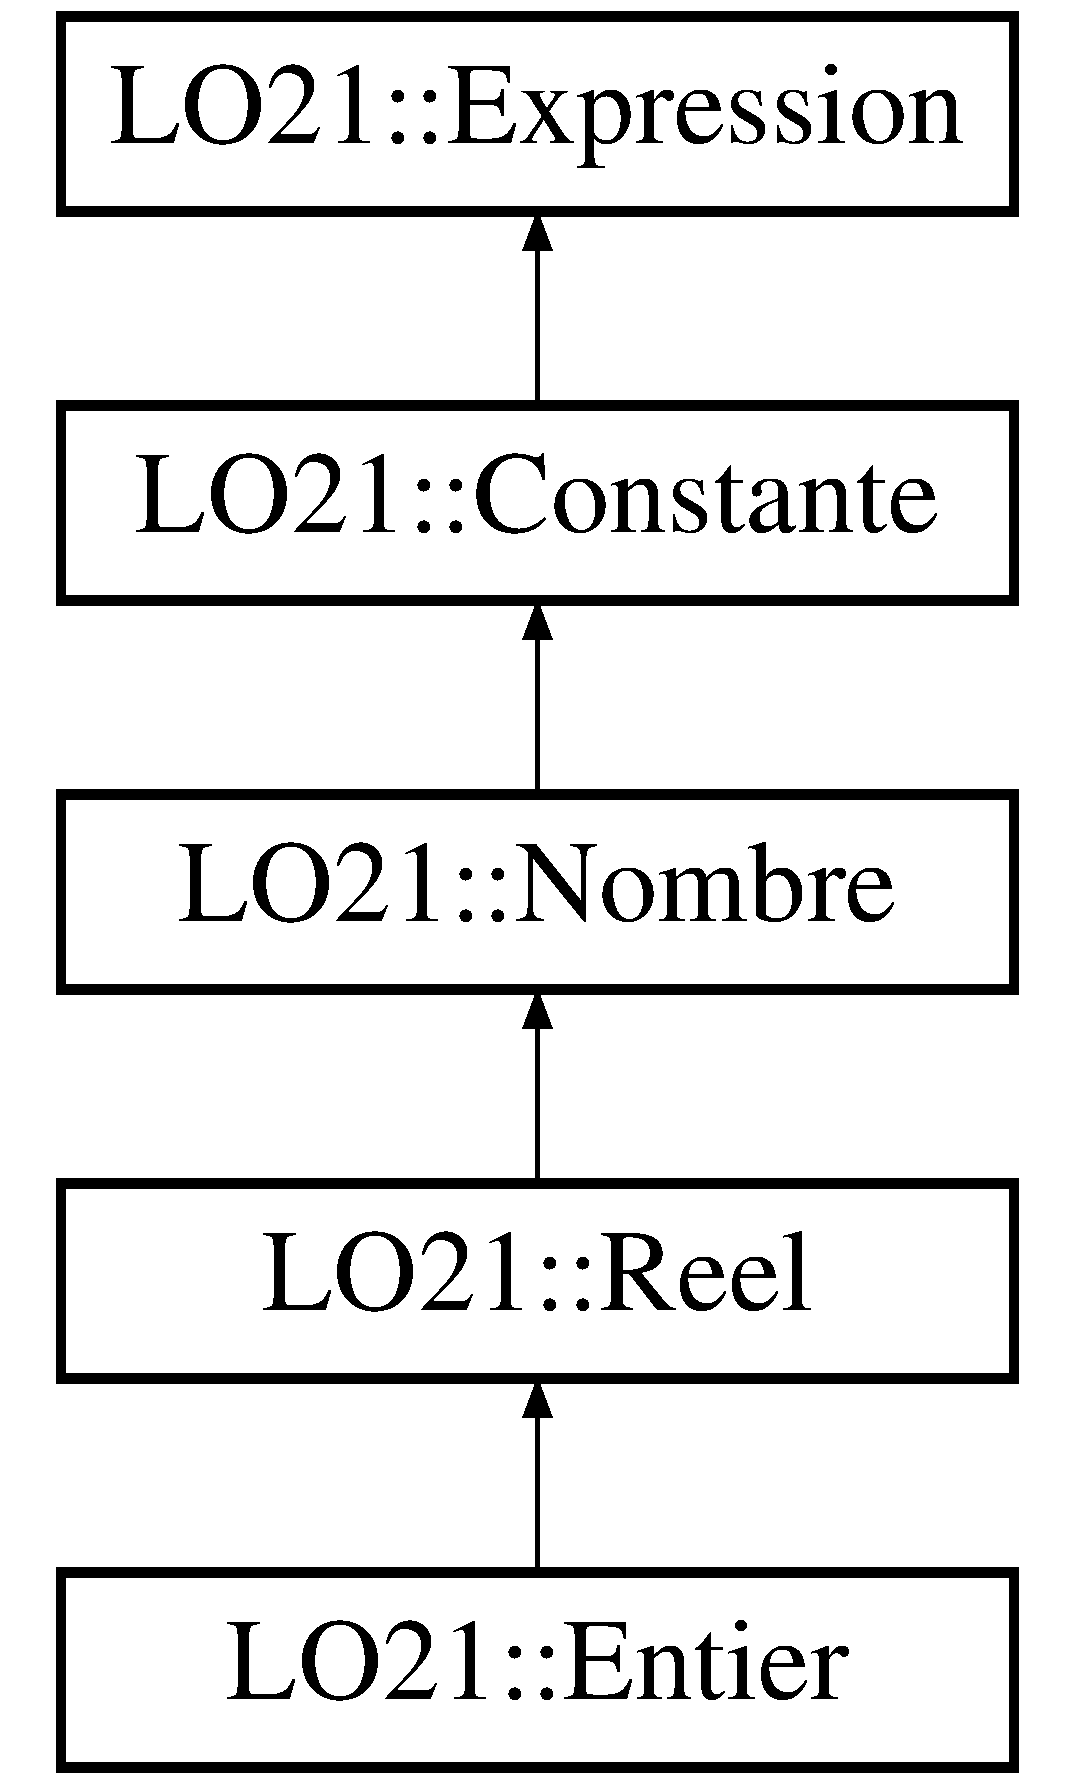
\includegraphics[height=5.000000cm]{class_l_o21_1_1_reel}
\end{center}
\end{figure}
\subsection*{\-Public \-Member \-Functions}
\begin{DoxyCompactItemize}
\item 
\hyperlink{class_l_o21_1_1_constante}{\-Constante} \& \hyperlink{class_l_o21_1_1_reel_ada705f00ece11942f330bad8497c2cb5}{addition} (const \hyperlink{class_l_o21_1_1_constante}{\-Constante} \&nb) const 
\begin{DoxyCompactList}\small\item\em \-Gere l'addition entre un reel et une constante quelle qu'elle soit. \end{DoxyCompactList}\item 
\hyperlink{class_l_o21_1_1_constante}{\-Constante} \& \hyperlink{class_l_o21_1_1_reel_a9e9ed5805f01d5661aa26c5f626e10ad}{soustraction} (const \hyperlink{class_l_o21_1_1_constante}{\-Constante} \&nb) const 
\begin{DoxyCompactList}\small\item\em \-Gere la soustraction entre un reel et une constante quelle qu'elle soit. \end{DoxyCompactList}\item 
\hyperlink{class_l_o21_1_1_constante}{\-Constante} \& \hyperlink{class_l_o21_1_1_reel_a01e5dc973684a30f98f7bde0d0c5840d}{multiplication} (const \hyperlink{class_l_o21_1_1_constante}{\-Constante} \&nb) const 
\begin{DoxyCompactList}\small\item\em \-Gere la multiplication entre un reel et une constante quelle qu'elle soit. \end{DoxyCompactList}\item 
\hyperlink{class_l_o21_1_1_constante}{\-Constante} \& \hyperlink{class_l_o21_1_1_reel_a2b4c6ae1d997ddd4e32e10e4511cfae0}{division} (const \hyperlink{class_l_o21_1_1_constante}{\-Constante} \&nb) const 
\begin{DoxyCompactList}\small\item\em \-Gere la division entre un reel et une constante quelle qu'elle soit. \end{DoxyCompactList}\item 
\-Q\-String \hyperlink{class_l_o21_1_1_reel_a3a9ad40b48c0fe365d69d023b026b34c}{to\-String} () const 
\begin{DoxyCompactList}\small\item\em \-Permet l'affichage du reel. \end{DoxyCompactList}\item 
\hyperlink{class_l_o21_1_1_rationnel}{\-Rationnel} \& \hyperlink{class_l_o21_1_1_reel_ada7096a46903e140082b945904018ca7}{to\-Rationnel} () const 
\begin{DoxyCompactList}\small\item\em \-Transforme un reel en rationnel. \end{DoxyCompactList}\item 
\hyperlink{class_l_o21_1_1_entier}{\-Entier} \& \hyperlink{class_l_o21_1_1_reel_aac90e89b0b11d89898fc5e6faf8ad2e4}{to\-Entier} () const 
\begin{DoxyCompactList}\small\item\em \-Transforme un reel en entier. \end{DoxyCompactList}\item 
\hyperlink{class_l_o21_1_1_complexe}{\-Complexe} \& \hyperlink{class_l_o21_1_1_reel_a9b50412d065606b01f322f94e5dd0639}{to\-Complexe} () const 
\begin{DoxyCompactList}\small\item\em \-Transforme un reel en nombre complexe. \end{DoxyCompactList}\item 
float \hyperlink{class_l_o21_1_1_reel_a2a989b2cac3a15ae99d22f39111f19c6}{get\-\_\-x} () const 
\begin{DoxyCompactList}\small\item\em \-Recupere la valeur du reel. \end{DoxyCompactList}\item 
\hyperlink{class_l_o21_1_1_reel_adf2ed2cbdebab95f05e2744c981d17f3}{\-Reel} (const double x=0.)
\begin{DoxyCompactList}\small\item\em \-Constructeur de la classe \hyperlink{class_l_o21_1_1_reel}{\-Reel}. \end{DoxyCompactList}\item 
\hyperlink{class_l_o21_1_1_reel}{\-Reel} $\ast$ \hyperlink{class_l_o21_1_1_reel_a03bf8d59ba75b2fc45d3db330210201a}{clone} () const 
\begin{DoxyCompactList}\small\item\em \-Fais une copie de l'objet appelant. \end{DoxyCompactList}\end{DoxyCompactItemize}


\subsection{\-Detailed \-Description}
\-Classe permettant de gerer les nombres reels. 

\subsection{\-Constructor \& \-Destructor \-Documentation}
\hypertarget{class_l_o21_1_1_reel_adf2ed2cbdebab95f05e2744c981d17f3}{\index{\-L\-O21\-::\-Reel@{\-L\-O21\-::\-Reel}!\-Reel@{\-Reel}}
\index{\-Reel@{\-Reel}!LO21::Reel@{\-L\-O21\-::\-Reel}}
\subsubsection[{\-Reel}]{\setlength{\rightskip}{0pt plus 5cm}{\bf \-L\-O21\-::\-Reel\-::\-Reel} (
\begin{DoxyParamCaption}
\item[{const double}]{x = {\ttfamily 0.}}
\end{DoxyParamCaption}
)\hspace{0.3cm}{\ttfamily  \mbox{[}inline\mbox{]}}}}\label{class_l_o21_1_1_reel_adf2ed2cbdebab95f05e2744c981d17f3}


\-Constructeur de la classe \hyperlink{class_l_o21_1_1_reel}{\-Reel}. 


\begin{DoxyParams}{\-Parameters}
{\em x} & un double afin d'instancier un objet \hyperlink{class_l_o21_1_1_reel}{\-Reel} \\
\hline
\end{DoxyParams}


\subsection{\-Member \-Function \-Documentation}
\hypertarget{class_l_o21_1_1_reel_ada705f00ece11942f330bad8497c2cb5}{\index{\-L\-O21\-::\-Reel@{\-L\-O21\-::\-Reel}!addition@{addition}}
\index{addition@{addition}!LO21::Reel@{\-L\-O21\-::\-Reel}}
\subsubsection[{addition}]{\setlength{\rightskip}{0pt plus 5cm}{\bf \-Constante} \& {\bf \-L\-O21\-::\-Reel\-::addition} (
\begin{DoxyParamCaption}
\item[{const {\bf \-Constante} \&}]{nb}
\end{DoxyParamCaption}
) const\hspace{0.3cm}{\ttfamily  \mbox{[}virtual\mbox{]}}}}\label{class_l_o21_1_1_reel_ada705f00ece11942f330bad8497c2cb5}


\-Gere l'addition entre un reel et une constante quelle qu'elle soit. 

\-Le nombre reel


\begin{DoxyParams}{\-Parameters}
{\em nb} & une reference vers une constante \\
\hline
\end{DoxyParams}
\begin{DoxyReturn}{\-Returns}
\hyperlink{class_l_o21_1_1_constante}{\-Constante}\& une reference vers la constante creee a partir du resultat 
\end{DoxyReturn}


\-Implements \hyperlink{class_l_o21_1_1_nombre_a75c7a5c063ed122f7ba004e09f1f6621}{\-L\-O21\-::\-Nombre}.



\-Reimplemented in \hyperlink{class_l_o21_1_1_entier_a8c70a23f95a29034d78fc5b8c76c4265}{\-L\-O21\-::\-Entier}.

\hypertarget{class_l_o21_1_1_reel_a03bf8d59ba75b2fc45d3db330210201a}{\index{\-L\-O21\-::\-Reel@{\-L\-O21\-::\-Reel}!clone@{clone}}
\index{clone@{clone}!LO21::Reel@{\-L\-O21\-::\-Reel}}
\subsubsection[{clone}]{\setlength{\rightskip}{0pt plus 5cm}{\bf \-Reel} $\ast$ {\bf \-L\-O21\-::\-Reel\-::clone} (
\begin{DoxyParamCaption}
{}
\end{DoxyParamCaption}
) const\hspace{0.3cm}{\ttfamily  \mbox{[}virtual\mbox{]}}}}\label{class_l_o21_1_1_reel_a03bf8d59ba75b2fc45d3db330210201a}


\-Fais une copie de l'objet appelant. 

\begin{DoxyReturn}{\-Returns}
\-Reel$\ast$ un pointeur vers le reel cree a partir de l'objet 
\end{DoxyReturn}


\-Implements \hyperlink{class_l_o21_1_1_nombre_aea071e3bcebfdc9337eaea8515e248c9}{\-L\-O21\-::\-Nombre}.



\-Reimplemented in \hyperlink{class_l_o21_1_1_entier_a76f8af45d660b33c6e082986be0a9223}{\-L\-O21\-::\-Entier}.

\hypertarget{class_l_o21_1_1_reel_a2b4c6ae1d997ddd4e32e10e4511cfae0}{\index{\-L\-O21\-::\-Reel@{\-L\-O21\-::\-Reel}!division@{division}}
\index{division@{division}!LO21::Reel@{\-L\-O21\-::\-Reel}}
\subsubsection[{division}]{\setlength{\rightskip}{0pt plus 5cm}{\bf \-Constante} \& {\bf \-L\-O21\-::\-Reel\-::division} (
\begin{DoxyParamCaption}
\item[{const {\bf \-Constante} \&}]{nb}
\end{DoxyParamCaption}
) const\hspace{0.3cm}{\ttfamily  \mbox{[}virtual\mbox{]}}}}\label{class_l_o21_1_1_reel_a2b4c6ae1d997ddd4e32e10e4511cfae0}


\-Gere la division entre un reel et une constante quelle qu'elle soit. 


\begin{DoxyParams}{\-Parameters}
{\em nb} & une reference vers une constante \\
\hline
\end{DoxyParams}
\begin{DoxyReturn}{\-Returns}
\hyperlink{class_l_o21_1_1_constante}{\-Constante}\& une reference vers la constante creee a partir du resultat 
\end{DoxyReturn}


\-Implements \hyperlink{class_l_o21_1_1_nombre_aafde3453c22512a8ca152f4013d0f08f}{\-L\-O21\-::\-Nombre}.



\-Reimplemented in \hyperlink{class_l_o21_1_1_entier_a4a9e09753bde4c527596c9a2cda8c87e}{\-L\-O21\-::\-Entier}.

\hypertarget{class_l_o21_1_1_reel_a2a989b2cac3a15ae99d22f39111f19c6}{\index{\-L\-O21\-::\-Reel@{\-L\-O21\-::\-Reel}!get\-\_\-x@{get\-\_\-x}}
\index{get\-\_\-x@{get\-\_\-x}!LO21::Reel@{\-L\-O21\-::\-Reel}}
\subsubsection[{get\-\_\-x}]{\setlength{\rightskip}{0pt plus 5cm}float {\bf \-L\-O21\-::\-Reel\-::get\-\_\-x} (
\begin{DoxyParamCaption}
{}
\end{DoxyParamCaption}
) const\hspace{0.3cm}{\ttfamily  \mbox{[}inline\mbox{]}}}}\label{class_l_o21_1_1_reel_a2a989b2cac3a15ae99d22f39111f19c6}


\-Recupere la valeur du reel. 

\begin{DoxyReturn}{\-Returns}
float contenant la valeur du reel 
\end{DoxyReturn}


\-Reimplemented in \hyperlink{class_l_o21_1_1_entier_a144f7ad9fd1d1de79503aa647c53d758}{\-L\-O21\-::\-Entier}.

\hypertarget{class_l_o21_1_1_reel_a01e5dc973684a30f98f7bde0d0c5840d}{\index{\-L\-O21\-::\-Reel@{\-L\-O21\-::\-Reel}!multiplication@{multiplication}}
\index{multiplication@{multiplication}!LO21::Reel@{\-L\-O21\-::\-Reel}}
\subsubsection[{multiplication}]{\setlength{\rightskip}{0pt plus 5cm}{\bf \-Constante} \& {\bf \-L\-O21\-::\-Reel\-::multiplication} (
\begin{DoxyParamCaption}
\item[{const {\bf \-Constante} \&}]{nb}
\end{DoxyParamCaption}
) const\hspace{0.3cm}{\ttfamily  \mbox{[}virtual\mbox{]}}}}\label{class_l_o21_1_1_reel_a01e5dc973684a30f98f7bde0d0c5840d}


\-Gere la multiplication entre un reel et une constante quelle qu'elle soit. 


\begin{DoxyParams}{\-Parameters}
{\em nb} & une reference vers une constante \\
\hline
\end{DoxyParams}
\begin{DoxyReturn}{\-Returns}
\hyperlink{class_l_o21_1_1_constante}{\-Constante}\& une reference vers la constante creee a partir du resultat 
\end{DoxyReturn}


\-Implements \hyperlink{class_l_o21_1_1_nombre_a63cf8dbd304585fe106e8eeebe8c4e89}{\-L\-O21\-::\-Nombre}.



\-Reimplemented in \hyperlink{class_l_o21_1_1_entier_a34fdbc8acc0a18318916312983dc78f9}{\-L\-O21\-::\-Entier}.

\hypertarget{class_l_o21_1_1_reel_a9e9ed5805f01d5661aa26c5f626e10ad}{\index{\-L\-O21\-::\-Reel@{\-L\-O21\-::\-Reel}!soustraction@{soustraction}}
\index{soustraction@{soustraction}!LO21::Reel@{\-L\-O21\-::\-Reel}}
\subsubsection[{soustraction}]{\setlength{\rightskip}{0pt plus 5cm}{\bf \-Constante} \& {\bf \-L\-O21\-::\-Reel\-::soustraction} (
\begin{DoxyParamCaption}
\item[{const {\bf \-Constante} \&}]{nb}
\end{DoxyParamCaption}
) const\hspace{0.3cm}{\ttfamily  \mbox{[}virtual\mbox{]}}}}\label{class_l_o21_1_1_reel_a9e9ed5805f01d5661aa26c5f626e10ad}


\-Gere la soustraction entre un reel et une constante quelle qu'elle soit. 


\begin{DoxyParams}{\-Parameters}
{\em nb} & une reference vers une constante \\
\hline
\end{DoxyParams}
\begin{DoxyReturn}{\-Returns}
\hyperlink{class_l_o21_1_1_constante}{\-Constante}\& une reference vers la constante creee a partir du resultat 
\end{DoxyReturn}


\-Implements \hyperlink{class_l_o21_1_1_nombre_a1e412b0e89c0b68c0ee04a3078c098b1}{\-L\-O21\-::\-Nombre}.



\-Reimplemented in \hyperlink{class_l_o21_1_1_entier_aa9ebbf0b51016b7e14a12909ed6ab7bb}{\-L\-O21\-::\-Entier}.

\hypertarget{class_l_o21_1_1_reel_a9b50412d065606b01f322f94e5dd0639}{\index{\-L\-O21\-::\-Reel@{\-L\-O21\-::\-Reel}!to\-Complexe@{to\-Complexe}}
\index{to\-Complexe@{to\-Complexe}!LO21::Reel@{\-L\-O21\-::\-Reel}}
\subsubsection[{to\-Complexe}]{\setlength{\rightskip}{0pt plus 5cm}{\bf \-Complexe} \& {\bf \-L\-O21\-::\-Reel\-::to\-Complexe} (
\begin{DoxyParamCaption}
{}
\end{DoxyParamCaption}
) const}}\label{class_l_o21_1_1_reel_a9b50412d065606b01f322f94e5dd0639}


\-Transforme un reel en nombre complexe. 

\begin{DoxyReturn}{\-Returns}
\hyperlink{class_l_o21_1_1_complexe}{\-Complexe}\& une reference vers le complexe cree a partir du reel 
\end{DoxyReturn}


\-Reimplemented in \hyperlink{class_l_o21_1_1_entier_abc46eb792359f8dc47785b12837571e3}{\-L\-O21\-::\-Entier}.

\hypertarget{class_l_o21_1_1_reel_aac90e89b0b11d89898fc5e6faf8ad2e4}{\index{\-L\-O21\-::\-Reel@{\-L\-O21\-::\-Reel}!to\-Entier@{to\-Entier}}
\index{to\-Entier@{to\-Entier}!LO21::Reel@{\-L\-O21\-::\-Reel}}
\subsubsection[{to\-Entier}]{\setlength{\rightskip}{0pt plus 5cm}{\bf \-Entier} \& {\bf \-L\-O21\-::\-Reel\-::to\-Entier} (
\begin{DoxyParamCaption}
{}
\end{DoxyParamCaption}
) const\hspace{0.3cm}{\ttfamily  \mbox{[}virtual\mbox{]}}}}\label{class_l_o21_1_1_reel_aac90e89b0b11d89898fc5e6faf8ad2e4}


\-Transforme un reel en entier. 

\begin{DoxyReturn}{\-Returns}
\hyperlink{class_l_o21_1_1_entier}{\-Entier}\& une reference vers l'entier cree a partir du reel 
\end{DoxyReturn}


\-Reimplemented from \hyperlink{class_l_o21_1_1_nombre_a50ad2148d1f0de749361329268117a25}{\-L\-O21\-::\-Nombre}.

\hypertarget{class_l_o21_1_1_reel_ada7096a46903e140082b945904018ca7}{\index{\-L\-O21\-::\-Reel@{\-L\-O21\-::\-Reel}!to\-Rationnel@{to\-Rationnel}}
\index{to\-Rationnel@{to\-Rationnel}!LO21::Reel@{\-L\-O21\-::\-Reel}}
\subsubsection[{to\-Rationnel}]{\setlength{\rightskip}{0pt plus 5cm}{\bf \-Rationnel} \& {\bf \-L\-O21\-::\-Reel\-::to\-Rationnel} (
\begin{DoxyParamCaption}
{}
\end{DoxyParamCaption}
) const\hspace{0.3cm}{\ttfamily  \mbox{[}virtual\mbox{]}}}}\label{class_l_o21_1_1_reel_ada7096a46903e140082b945904018ca7}


\-Transforme un reel en rationnel. 

\begin{DoxyReturn}{\-Returns}
\hyperlink{class_l_o21_1_1_rationnel}{\-Rationnel}\& une reference vers le rationnel cree a partir du reel 
\end{DoxyReturn}


\-Reimplemented from \hyperlink{class_l_o21_1_1_nombre_a89c9efd6230695a6ace9605a2a82ee96}{\-L\-O21\-::\-Nombre}.



\-Reimplemented in \hyperlink{class_l_o21_1_1_entier_a1039b5ecf2ba82f2f8967d52eb81e2b2}{\-L\-O21\-::\-Entier}.

\hypertarget{class_l_o21_1_1_reel_a3a9ad40b48c0fe365d69d023b026b34c}{\index{\-L\-O21\-::\-Reel@{\-L\-O21\-::\-Reel}!to\-String@{to\-String}}
\index{to\-String@{to\-String}!LO21::Reel@{\-L\-O21\-::\-Reel}}
\subsubsection[{to\-String}]{\setlength{\rightskip}{0pt plus 5cm}\-Q\-String {\bf \-L\-O21\-::\-Reel\-::to\-String} (
\begin{DoxyParamCaption}
{}
\end{DoxyParamCaption}
) const\hspace{0.3cm}{\ttfamily  \mbox{[}virtual\mbox{]}}}}\label{class_l_o21_1_1_reel_a3a9ad40b48c0fe365d69d023b026b34c}


\-Permet l'affichage du reel. 

\begin{DoxyReturn}{\-Returns}
\-Q\-String contenant le texte representant le reel 
\end{DoxyReturn}


\-Implements \hyperlink{class_l_o21_1_1_nombre_a081a338b80d4f51048c0729597708c24}{\-L\-O21\-::\-Nombre}.



\-Reimplemented in \hyperlink{class_l_o21_1_1_entier_a8741d3caf244a1993d478b7353b5a65e}{\-L\-O21\-::\-Entier}.



\-The documentation for this class was generated from the following files\-:\begin{DoxyCompactItemize}
\item 
\hyperlink{_reel_8h}{\-Reel.\-h}\item 
\-Reel.\-cpp\end{DoxyCompactItemize}

\hypertarget{classvirtual}{\section{virtual \-Class \-Reference}
\label{classvirtual}\index{virtual@{virtual}}
}


\-Permet d'afficher sous forme textuelle les objets \-Expression.  




\subsection{\-Detailed \-Description}
\-Permet d'afficher sous forme textuelle les objets \-Expression. 

() const \begin{DoxyReturn}{\-Returns}
\-Q\-String contenant le texte definissant l'objet \-Expression 
\end{DoxyReturn}


\-The documentation for this class was generated from the following file\-:\begin{DoxyCompactItemize}
\item 
\hyperlink{_expression_8h}{\-Expression.\-h}\end{DoxyCompactItemize}

\hypertarget{classvirtual}{\section{virtual \-Class \-Reference}
\label{classvirtual}\index{virtual@{virtual}}
}


\-Permet d'afficher sous forme textuelle les objets \-Expression.  




\subsection{\-Detailed \-Description}
\-Permet d'afficher sous forme textuelle les objets \-Expression. 

() const \begin{DoxyReturn}{\-Returns}
\-Q\-String contenant le texte definissant l'objet \-Expression 
\end{DoxyReturn}


\-The documentation for this class was generated from the following file\-:\begin{DoxyCompactItemize}
\item 
\hyperlink{_expression_8h}{\-Expression.\-h}\end{DoxyCompactItemize}

\chapter{\-File \-Documentation}
\hypertarget{_calculatrice_8h}{\section{\-Calculatrice.\-h \-File \-Reference}
\label{_calculatrice_8h}\index{\-Calculatrice.\-h@{\-Calculatrice.\-h}}
}


\-Fichier d'en-\/tete pour declaration de la classe \-Calculatrice.  


{\ttfamily \#include \char`\"{}\-Pile.\-h\char`\"{}}\*
{\ttfamily \#include \char`\"{}\-Fabrique.\-h\char`\"{}}\*
{\ttfamily \#include \char`\"{}\-Gardien.\-h\char`\"{}}\*
{\ttfamily \#include \char`\"{}\-Log\-System.\-h\char`\"{}}\*
\subsection*{\-Classes}
\begin{DoxyCompactItemize}
\item 
class \hyperlink{class_l_o21_1_1_calculatrice}{\-L\-O21\-::\-Calculatrice}
\end{DoxyCompactItemize}
\subsection*{\-Namespaces}
\begin{DoxyCompactItemize}
\item 
namespace \hyperlink{namespace_l_o21}{\-L\-O21}
\begin{DoxyCompactList}\small\item\em \-Designe les classes definies dans le but du projet de \hyperlink{namespace_l_o21}{\-L\-O21} \-P12. \end{DoxyCompactList}\end{DoxyCompactItemize}


\subsection{\-Detailed \-Description}
\-Fichier d'en-\/tete pour declaration de la classe \-Calculatrice. \-Fichier d'en-\/tete pour declaration de la classe \-Fabrique.

\begin{DoxyAuthor}{\-Author}
\-Florian \-Dambrine, \-Olivia \-Reaney 
\end{DoxyAuthor}

\hypertarget{_calculatrice_exception_8h}{\section{\-Calculatrice\-Exception.\-h \-File \-Reference}
\label{_calculatrice_exception_8h}\index{\-Calculatrice\-Exception.\-h@{\-Calculatrice\-Exception.\-h}}
}


\-Fichier d'en-\/tete pour declaration de la classe \-Calculatrice\-Exception.  


{\ttfamily \#include $<$\-Q\-String$>$}\*
{\ttfamily \#include $<$stdexcept$>$}\*
\subsection*{\-Classes}
\begin{DoxyCompactItemize}
\item 
class \hyperlink{class_l_o21_1_1_calculatrice_exception}{\-L\-O21\-::\-Calculatrice\-Exception}
\begin{DoxyCompactList}\small\item\em \-Classe gerant l'affichage des erreurs, et la levee d'exceptions. \end{DoxyCompactList}\end{DoxyCompactItemize}
\subsection*{\-Namespaces}
\begin{DoxyCompactItemize}
\item 
namespace \hyperlink{namespace_l_o21}{\-L\-O21}
\begin{DoxyCompactList}\small\item\em \-Designe les classes definies dans le but du projet de \hyperlink{namespace_l_o21}{\-L\-O21} \-P12. \end{DoxyCompactList}\end{DoxyCompactItemize}
\subsection*{\-Enumerations}
\begin{DoxyCompactItemize}
\item 
enum \hyperlink{namespace_l_o21_a4cea05b79a8da799daea8141505d6f59}{\-L\-O21\-::\-Calculatrice\-Exception\-Type} \{ {\bfseries \-M\-A\-T\-H\-S}, 
{\bfseries \-O\-T\-H\-E\-R}, 
{\bfseries \-P\-I\-L\-E}, 
{\bfseries \-O\-P\-T\-I\-O\-N}
 \}
\end{DoxyCompactItemize}


\subsection{\-Detailed \-Description}
\-Fichier d'en-\/tete pour declaration de la classe \-Calculatrice\-Exception. \begin{DoxyAuthor}{\-Author}
\-Florian \-Dambrine, \-Olivia \-Reaney 
\end{DoxyAuthor}

\hypertarget{_complexe_8h}{\section{\-Complexe.\-h \-File \-Reference}
\label{_complexe_8h}\index{\-Complexe.\-h@{\-Complexe.\-h}}
}


\-Fichier d'en-\/tete pour declaration de la classe \hyperlink{class_complexe}{\-Complexe}.  


{\ttfamily \#include $<$iostream$>$}\*
{\ttfamily \#include \char`\"{}\-Constante.\-h\char`\"{}}\*
{\ttfamily \#include \char`\"{}\-Nombre.\-h\char`\"{}}\*
{\ttfamily \#include $<$typeinfo$>$}\*
{\ttfamily \#include $<$\-Q\-String$>$}\*
\subsection*{\-Classes}
\begin{DoxyCompactItemize}
\item 
class \hyperlink{class_l_o21_1_1_complexe}{\-L\-O21\-::\-Complexe}
\begin{DoxyCompactList}\small\item\em \-Classe permettant de gerer les nombres complexes. \end{DoxyCompactList}\end{DoxyCompactItemize}
\subsection*{\-Namespaces}
\begin{DoxyCompactItemize}
\item 
namespace \hyperlink{namespace_l_o21}{\-L\-O21}
\begin{DoxyCompactList}\small\item\em \-Designe les classes definies dans le but du projet de \hyperlink{namespace_l_o21}{\-L\-O21} \-P12. \end{DoxyCompactList}\end{DoxyCompactItemize}


\subsection{\-Detailed \-Description}
\-Fichier d'en-\/tete pour declaration de la classe \hyperlink{class_complexe}{\-Complexe}. \begin{DoxyAuthor}{\-Author}
\-Florian \-Dambrine, \-Olivia \-Reaney 
\end{DoxyAuthor}

\hypertarget{_constante_8h}{\section{\-Constante.\-h \-File \-Reference}
\label{_constante_8h}\index{\-Constante.\-h@{\-Constante.\-h}}
}


\-Fichier d'en-\/tete pour declaration de la classe \-Constante.  


{\ttfamily \#include $<$\-Q\-Debug$>$}\*
{\ttfamily \#include \char`\"{}\-Expression.\-h\char`\"{}}\*
\subsection*{\-Classes}
\begin{DoxyCompactItemize}
\item 
class \hyperlink{class_l_o21_1_1_constante}{\-L\-O21\-::\-Constante}
\begin{DoxyCompactList}\small\item\em \-Definit d'une maniere generale les operations possibles sur les constantes qu'elles soient entieres, reelles, rationnelles ou complexes. \end{DoxyCompactList}\end{DoxyCompactItemize}
\subsection*{\-Namespaces}
\begin{DoxyCompactItemize}
\item 
namespace \hyperlink{namespace_l_o21}{\-L\-O21}
\begin{DoxyCompactList}\small\item\em \-Designe les classes definies dans le but du projet de \hyperlink{namespace_l_o21}{\-L\-O21} \-P12. \end{DoxyCompactList}\end{DoxyCompactItemize}


\subsection{\-Detailed \-Description}
\-Fichier d'en-\/tete pour declaration de la classe \-Constante. \begin{DoxyAuthor}{\-Author}
\-Florian \-Dambrine, \-Olivia \-Reaney 
\end{DoxyAuthor}

\hypertarget{_entier_8h}{\section{\-Entier.\-h \-File \-Reference}
\label{_entier_8h}\index{\-Entier.\-h@{\-Entier.\-h}}
}


\-Fichier d'en-\/tete pour declaration de la classe \-Entier.  


{\ttfamily \#include $<$iostream$>$}\*
{\ttfamily \#include $<$typeinfo$>$}\*
{\ttfamily \#include \char`\"{}\-Reel.\-h\char`\"{}}\*
{\ttfamily \#include \char`\"{}\-Calculatrice\-Exception.\-h\char`\"{}}\*
\subsection*{\-Classes}
\begin{DoxyCompactItemize}
\item 
class \hyperlink{class_l_o21_1_1_entier}{\-L\-O21\-::\-Entier}
\begin{DoxyCompactList}\small\item\em \-Classe representant un entier \-La classe gere les operations sur les entiers positifs et negatifs. \end{DoxyCompactList}\end{DoxyCompactItemize}
\subsection*{\-Namespaces}
\begin{DoxyCompactItemize}
\item 
namespace \hyperlink{namespace_l_o21}{\-L\-O21}
\begin{DoxyCompactList}\small\item\em \-Designe les classes definies dans le but du projet de \hyperlink{namespace_l_o21}{\-L\-O21} \-P12. \end{DoxyCompactList}\end{DoxyCompactItemize}
\subsection*{\-Functions}
\begin{DoxyCompactItemize}
\item 
int \hyperlink{_entier_8h_acf8e9299cf32eef32d8461cd7c1cb8c4}{factorielle} (int n)
\begin{DoxyCompactList}\small\item\em \-Execute la factorielle du nombre n passe en argument. \end{DoxyCompactList}\end{DoxyCompactItemize}


\subsection{\-Detailed \-Description}
\-Fichier d'en-\/tete pour declaration de la classe \-Entier. \-Fichier d'en-\/tete pour declaration de la classe \-Log\-System.

\-Fichier d'en-\/tete pour declaration de la classe \-Log\-Message.

\begin{DoxyAuthor}{\-Author}
\-Florian \-Dambrine, \-Olivia \-Reaney 
\end{DoxyAuthor}


\subsection{\-Function \-Documentation}
\hypertarget{_entier_8h_acf8e9299cf32eef32d8461cd7c1cb8c4}{\index{\-Entier.\-h@{\-Entier.\-h}!factorielle@{factorielle}}
\index{factorielle@{factorielle}!Entier.h@{\-Entier.\-h}}
\subsubsection[{factorielle}]{\setlength{\rightskip}{0pt plus 5cm}int {\bf factorielle} (
\begin{DoxyParamCaption}
\item[{int}]{n}
\end{DoxyParamCaption}
)}}\label{_entier_8h_acf8e9299cf32eef32d8461cd7c1cb8c4}


\-Execute la factorielle du nombre n passe en argument. 


\begin{DoxyParams}{\-Parameters}
{\em n} & \-Entier a partir duquel la factorielle va etre calculee \\
\hline
\end{DoxyParams}
\begin{DoxyReturn}{\-Returns}
int le resultat de la factorielle 
\end{DoxyReturn}

\hypertarget{_exp_8h}{\section{\-Exp.\-h \-File \-Reference}
\label{_exp_8h}\index{\-Exp.\-h@{\-Exp.\-h}}
}


\-Fichier d'en-\/tete pour declaration de la classe \-Exp.  


{\ttfamily \#include \char`\"{}\-Constante.\-h\char`\"{}}\*
{\ttfamily \#include \char`\"{}\-Fabrique.\-h\char`\"{}}\*
\subsection*{\-Classes}
\begin{DoxyCompactItemize}
\item 
class \hyperlink{class_l_o21_1_1_exp}{\-L\-O21\-::\-Exp}
\begin{DoxyCompactList}\small\item\em \-Classe permettant de gerer les expressions entre ' ' a evaluer plus tard. \end{DoxyCompactList}\end{DoxyCompactItemize}
\subsection*{\-Namespaces}
\begin{DoxyCompactItemize}
\item 
namespace \hyperlink{namespace_l_o21}{\-L\-O21}
\begin{DoxyCompactList}\small\item\em \-Designe les classes definies dans le but du projet de \hyperlink{namespace_l_o21}{\-L\-O21} \-P12. \end{DoxyCompactList}\end{DoxyCompactItemize}


\subsection{\-Detailed \-Description}
\-Fichier d'en-\/tete pour declaration de la classe \-Exp. \begin{DoxyAuthor}{\-Author}
\-Florian \-Dambrine, \-Olivia \-Reaney 
\end{DoxyAuthor}

\hypertarget{_expression_8h}{\section{\-Expression.\-h \-File \-Reference}
\label{_expression_8h}\index{\-Expression.\-h@{\-Expression.\-h}}
}


\-Fichier d'en-\/tete pour declaration de la classe \-Expression.  


{\ttfamily \#include $<$\-Q\-Text\-Stream$>$}\*
\subsection*{\-Classes}
\begin{DoxyCompactItemize}
\item 
class \hyperlink{class_l_o21_1_1_expression}{\-L\-O21\-::\-Expression}
\begin{DoxyCompactList}\small\item\em \-Classe permettant d'encapsuler des \-Constantes et des \-Operateurs pour les stocker dans la pile. \end{DoxyCompactList}\end{DoxyCompactItemize}
\subsection*{\-Namespaces}
\begin{DoxyCompactItemize}
\item 
namespace \hyperlink{namespace_l_o21}{\-L\-O21}
\begin{DoxyCompactList}\small\item\em \-Designe les classes definies dans le but du projet de \hyperlink{namespace_l_o21}{\-L\-O21} \-P12. \end{DoxyCompactList}\end{DoxyCompactItemize}
\subsection*{\-Functions}
\begin{DoxyCompactItemize}
\item 
\-Q\-Text\-Stream \& \hyperlink{_expression_8h_a5d1803bd897688d2923c7b3f696981a7}{operator$<$$<$} (\-Q\-Text\-Stream \&s, const \hyperlink{class_l_o21_1_1_expression}{\-L\-O21\-::\-Expression} \&n)
\begin{DoxyCompactList}\small\item\em \-Classe permettant de gerer les nombres complexes. \end{DoxyCompactList}\end{DoxyCompactItemize}


\subsection{\-Detailed \-Description}
\-Fichier d'en-\/tete pour declaration de la classe \-Expression. \begin{DoxyAuthor}{\-Author}
\-Florian \-Dambrine, \-Olivia \-Reaney 
\end{DoxyAuthor}


\subsection{\-Function \-Documentation}
\hypertarget{_expression_8h_a5d1803bd897688d2923c7b3f696981a7}{\index{\-Expression.\-h@{\-Expression.\-h}!operator$<$$<$@{operator$<$$<$}}
\index{operator$<$$<$@{operator$<$$<$}!Expression.h@{\-Expression.\-h}}
\subsubsection[{operator$<$$<$}]{\setlength{\rightskip}{0pt plus 5cm}\-Q\-Text\-Stream\& operator$<$$<$ (
\begin{DoxyParamCaption}
\item[{\-Q\-Text\-Stream \&}]{s, }
\item[{const {\bf \-L\-O21\-::\-Expression} \&}]{e}
\end{DoxyParamCaption}
)}}\label{_expression_8h_a5d1803bd897688d2923c7b3f696981a7}


\-Classe permettant de gerer les nombres complexes. 


\begin{DoxyParams}{\-Parameters}
{\em s} & \\
\hline
{\em n} & \\
\hline
\end{DoxyParams}
\begin{DoxyReturn}{\-Returns}
\-Q\-Text\-Stream\& 
\end{DoxyReturn}

\hypertarget{_gardien_8h}{\section{\-Gardien.\-h \-File \-Reference}
\label{_gardien_8h}\index{\-Gardien.\-h@{\-Gardien.\-h}}
}


\-Fichier d'en-\/tete pour declaration de la classe \-Gardien.  


{\ttfamily \#include $<$\-Q\-String$>$}\*
{\ttfamily \#include $<$\-Q\-Stack$>$}\*
{\ttfamily \#include \char`\"{}\-Pile.\-h\char`\"{}}\*
\subsection*{\-Classes}
\begin{DoxyCompactItemize}
\item 
class \hyperlink{class_l_o21_1_1_gardien}{\-L\-O21\-::\-Gardien}
\begin{DoxyCompactList}\small\item\em \-Classe qui s'occupe de gerer les operations d'undo redo grace a l'implementation d'un design pattern \-Memento. \end{DoxyCompactList}\end{DoxyCompactItemize}
\subsection*{\-Namespaces}
\begin{DoxyCompactItemize}
\item 
namespace \hyperlink{namespace_l_o21}{\-L\-O21}
\begin{DoxyCompactList}\small\item\em \-Designe les classes definies dans le but du projet de \hyperlink{namespace_l_o21}{\-L\-O21} \-P12. \end{DoxyCompactList}\end{DoxyCompactItemize}


\subsection{\-Detailed \-Description}
\-Fichier d'en-\/tete pour declaration de la classe \-Gardien. \begin{DoxyAuthor}{\-Author}
\-Florian \-Dambrine, \-Olivia \-Reaney 
\end{DoxyAuthor}

\hypertarget{mainwindow_8h}{\section{mainwindow.\-h \-File \-Reference}
\label{mainwindow_8h}\index{mainwindow.\-h@{mainwindow.\-h}}
}


\-Fichier d'en-\/t�te pour d�claration de la classe mainwindow.  


{\ttfamily \#include $<$\-Q\-Main\-Window$>$}\*
{\ttfamily \#include $<$\-Q\-Message\-Box$>$}\*
{\ttfamily \#include $<$\-Q\-Debug$>$}\*
{\ttfamily \#include $<$\-Q\-File$>$}\*
{\ttfamily \#include $<$\-Q\-Dir$>$}\*
{\ttfamily \#include $<$stdexcept$>$}\*
{\ttfamily \#include \char`\"{}\-Calculatrice.\-h\char`\"{}}\*
{\ttfamily \#include \char`\"{}\-Fabrique.\-h\char`\"{}}\*
{\ttfamily \#include \char`\"{}\-Pile.\-h\char`\"{}}\*
{\ttfamily \#include \char`\"{}\-Option.\-h\char`\"{}}\*
{\ttfamily \#include \char`\"{}\-Expression.\-h\char`\"{}}\*
{\ttfamily \#include \char`\"{}\-Log\-System.\-h\char`\"{}}\*
\subsection*{\-Classes}
\begin{DoxyCompactItemize}
\item 
class \hyperlink{class_main_window}{\-Main\-Window}
\begin{DoxyCompactList}\small\item\em \-Classe construisant l'interface de la calculatrice et g�rant les actions effectu�es par l'utilisateur. \end{DoxyCompactList}\end{DoxyCompactItemize}
\subsection*{\-Namespaces}
\begin{DoxyCompactItemize}
\item 
namespace \hyperlink{namespace_ui}{\-Ui}
\begin{DoxyCompactList}\small\item\em \-D�signe les classes d�finies dans le but du projet de \hyperlink{namespace_l_o21}{\-L\-O21} \-P12, concernant l'affichage de la calculatrice. \end{DoxyCompactList}\end{DoxyCompactItemize}


\subsection{\-Detailed \-Description}
\-Fichier d'en-\/t�te pour d�claration de la classe mainwindow. \begin{DoxyAuthor}{\-Author}
\-Florian \-Dambrine, \-Olivia \-Reaney 
\end{DoxyAuthor}

\hypertarget{_nombre_8h}{\section{\-Nombre.\-h \-File \-Reference}
\label{_nombre_8h}\index{\-Nombre.\-h@{\-Nombre.\-h}}
}


\-Fichier d'en-\/tete pour declaration de la classe \-Nombre.  


{\ttfamily \#include $<$\-Q\-String$>$}\*
{\ttfamily \#include \char`\"{}\-Constante.\-h\char`\"{}}\*
{\ttfamily \#include \char`\"{}\-Calculatrice\-Exception.\-h\char`\"{}}\*
{\ttfamily \#include \char`\"{}\-Option.\-h\char`\"{}}\*
{\ttfamily \#include \char`\"{}\-Log\-System.\-h\char`\"{}}\*
\subsection*{\-Classes}
\begin{DoxyCompactItemize}
\item 
class \hyperlink{class_l_o21_1_1_nombre}{\-L\-O21\-::\-Nombre}
\begin{DoxyCompactList}\small\item\em \-Classe encapsulant les classes \hyperlink{class_l_o21_1_1_entier}{\-Entier}, \hyperlink{class_l_o21_1_1_rationnel}{\-Rationnel} et \hyperlink{class_l_o21_1_1_reel}{\-Reel}. \end{DoxyCompactList}\end{DoxyCompactItemize}
\subsection*{\-Namespaces}
\begin{DoxyCompactItemize}
\item 
namespace \hyperlink{namespace_l_o21}{\-L\-O21}
\begin{DoxyCompactList}\small\item\em \-Designe les classes definies dans le but du projet de \hyperlink{namespace_l_o21}{\-L\-O21} \-P12. \end{DoxyCompactList}\end{DoxyCompactItemize}


\subsection{\-Detailed \-Description}
\-Fichier d'en-\/tete pour declaration de la classe \-Nombre. \begin{DoxyAuthor}{\-Author}
\-Florian \-Dambrine, \-Olivia \-Reaney 
\end{DoxyAuthor}

\hypertarget{_operateur_8h}{\section{\-Operateur.\-h \-File \-Reference}
\label{_operateur_8h}\index{\-Operateur.\-h@{\-Operateur.\-h}}
}


\-Fichier d'en-\/tete pour declaration de la classe \-Operateur.  


{\ttfamily \#include $<$stdexcept$>$}\*
{\ttfamily \#include $<$\-Q\-String$>$}\*
{\ttfamily \#include $<$\-Q\-String\-List$>$}\*
{\ttfamily \#include \char`\"{}\-Expression.\-h\char`\"{}}\*
{\ttfamily \#include \char`\"{}\-Fabrique.\-h\char`\"{}}\*
{\ttfamily \#include \char`\"{}\-Pile.\-h\char`\"{}}\*
{\ttfamily \#include \char`\"{}\-Calculatrice.\-h\char`\"{}}\*
\subsection*{\-Classes}
\begin{DoxyCompactItemize}
\item 
class \hyperlink{class_l_o21_1_1_operateur}{\-L\-O21\-::\-Operateur}
\begin{DoxyCompactList}\small\item\em \-Classe permettant de gerer les differents types d'operateurs. \end{DoxyCompactList}\end{DoxyCompactItemize}
\subsection*{\-Namespaces}
\begin{DoxyCompactItemize}
\item 
namespace \hyperlink{namespace_l_o21}{\-L\-O21}
\begin{DoxyCompactList}\small\item\em \-Designe les classes definies dans le but du projet de \hyperlink{namespace_l_o21}{\-L\-O21} \-P12. \end{DoxyCompactList}\end{DoxyCompactItemize}
\subsection*{\-Enumerations}
\begin{DoxyCompactItemize}
\item 
enum \hyperlink{namespace_l_o21_ad50ab07e90eb3964a086c2f7d95fb8d2}{\-L\-O21\-::enum\-Operateurs} \{ \*
{\bfseries \-A\-D\-D}, 
{\bfseries \-M\-U\-L}, 
{\bfseries \-S\-O\-U}, 
{\bfseries \-D\-I\-V}, 
\*
{\bfseries \-C\-O\-S}, 
{\bfseries \-S\-I\-N}, 
{\bfseries \-T\-A\-N}, 
{\bfseries \-C\-O\-S\-H}, 
\*
{\bfseries \-S\-I\-N\-H}, 
{\bfseries \-T\-A\-N\-H}, 
{\bfseries \-S\-Q\-R}, 
{\bfseries \-C\-U\-B\-E}, 
\*
{\bfseries \-S\-Q\-R\-T}, 
{\bfseries \-I\-N\-V}, 
{\bfseries \-S\-I\-G\-N}, 
{\bfseries \-L\-N}, 
\*
{\bfseries \-L\-O\-G}, 
{\bfseries \-P\-O\-W}, 
{\bfseries \-F\-A\-C\-T}, 
{\bfseries \-M\-O\-D}, 
\*
{\bfseries \-E\-V\-A\-L\-U\-A\-T\-I\-O\-N}
 \}
\begin{DoxyCompactList}\small\item\em \-Definit tous les types d'operateurs possibles dans une expression. \end{DoxyCompactList}\end{DoxyCompactItemize}


\subsection{\-Detailed \-Description}
\-Fichier d'en-\/tete pour declaration de la classe \-Operateur. \begin{DoxyAuthor}{\-Author}
\-Florian \-Dambrine, \-Olivia \-Reaney 
\end{DoxyAuthor}

\hypertarget{_operateur_binaire_8h}{\section{\-Operateur\-Binaire.\-h \-File \-Reference}
\label{_operateur_binaire_8h}\index{\-Operateur\-Binaire.\-h@{\-Operateur\-Binaire.\-h}}
}


\-Fichier d'en-\/tete pour declaration de la classe \-Operateur\-Binaire.  


{\ttfamily \#include \char`\"{}\-Operateur.\-h\char`\"{}}\*
{\ttfamily \#include \char`\"{}\-Expression.\-h\char`\"{}}\*
{\ttfamily \#include $<$iostream$>$}\*
{\ttfamily \#include $<$\-Q\-String$>$}\*
{\ttfamily \#include $<$typeinfo$>$}\*
\subsection*{\-Classes}
\begin{DoxyCompactItemize}
\item 
class \hyperlink{class_l_o21_1_1_operateur_binaire}{\-L\-O21\-::\-Operateur\-Binaire}
\begin{DoxyCompactList}\small\item\em \-Classe permettant de gerer les operateurs binaires presents dans une expression. \end{DoxyCompactList}\end{DoxyCompactItemize}
\subsection*{\-Namespaces}
\begin{DoxyCompactItemize}
\item 
namespace \hyperlink{namespace_l_o21}{\-L\-O21}
\begin{DoxyCompactList}\small\item\em \-Designe les classes definies dans le but du projet de \hyperlink{namespace_l_o21}{\-L\-O21} \-P12. \end{DoxyCompactList}\end{DoxyCompactItemize}


\subsection{\-Detailed \-Description}
\-Fichier d'en-\/tete pour declaration de la classe \-Operateur\-Binaire. \begin{DoxyAuthor}{\-Author}
\-Florian \-Dambrine, \-Olivia \-Reaney 
\end{DoxyAuthor}

\hypertarget{_operateur_unaire_8h}{\section{\-Operateur\-Unaire.\-h \-File \-Reference}
\label{_operateur_unaire_8h}\index{\-Operateur\-Unaire.\-h@{\-Operateur\-Unaire.\-h}}
}


\-Fichier d'en-\/tete pour declaration de la classe \-Operateur\-Unaire.  


{\ttfamily \#include \char`\"{}\-Operateur.\-h\char`\"{}}\*
{\ttfamily \#include \char`\"{}\-Expression.\-h\char`\"{}}\*
{\ttfamily \#include $<$\-Q\-String$>$}\*
\subsection*{\-Classes}
\begin{DoxyCompactItemize}
\item 
class \hyperlink{class_l_o21_1_1_operateur_unaire}{\-L\-O21\-::\-Operateur\-Unaire}
\begin{DoxyCompactList}\small\item\em \-Classe permettant de gerer les operateurs unaires presents dans une expression. \end{DoxyCompactList}\end{DoxyCompactItemize}
\subsection*{\-Namespaces}
\begin{DoxyCompactItemize}
\item 
namespace \hyperlink{namespace_l_o21}{\-L\-O21}
\begin{DoxyCompactList}\small\item\em \-Designe les classes definies dans le but du projet de \hyperlink{namespace_l_o21}{\-L\-O21} \-P12. \end{DoxyCompactList}\end{DoxyCompactItemize}


\subsection{\-Detailed \-Description}
\-Fichier d'en-\/tete pour declaration de la classe \-Operateur\-Unaire. \begin{DoxyAuthor}{\-Author}
\-Florian \-Dambrine, \-Olivia \-Reaney 
\end{DoxyAuthor}

\hypertarget{_option_8h}{\section{\-Option.\-h \-File \-Reference}
\label{_option_8h}\index{\-Option.\-h@{\-Option.\-h}}
}


\-Fichier d'en-\/tete pour declaration de la classe \-Option.  


{\ttfamily \#include $<$\-Q\-String$>$}\*
{\ttfamily \#include $<$\-Q\-Text\-Stream$>$}\*
{\ttfamily \#include $<$typeinfo$>$}\*
{\ttfamily \#include $<$\-Q\-File$>$}\*
{\ttfamily \#include \char`\"{}\-Calculatrice\-Exception.\-h\char`\"{}}\*
{\ttfamily \#include \char`\"{}\-Log\-System.\-h\char`\"{}}\*
\subsection*{\-Classes}
\begin{DoxyCompactItemize}
\item 
class \hyperlink{class_l_o21_1_1_option}{\-L\-O21\-::\-Option}
\begin{DoxyCompactList}\small\item\em \-Classe permettant de gerer les options gerees par l'utilisateur, implementant le design pattern \-Singleton. \end{DoxyCompactList}\end{DoxyCompactItemize}
\subsection*{\-Namespaces}
\begin{DoxyCompactItemize}
\item 
namespace \hyperlink{namespace_l_o21}{\-L\-O21}
\begin{DoxyCompactList}\small\item\em \-Designe les classes definies dans le but du projet de \hyperlink{namespace_l_o21}{\-L\-O21} \-P12. \end{DoxyCompactList}\end{DoxyCompactItemize}
\subsection*{\-Enumerations}
\begin{DoxyCompactItemize}
\item 
enum \hyperlink{_option_8h_aa88892c4cb734ae333411b4409f27f72}{\-Type\-Div} \{ {\bfseries \-M\-E\-N\-U\-\_\-\-E\-N\-T\-I\-E\-R}, 
{\bfseries \-M\-E\-N\-U\-\_\-\-R\-E\-E\-L}, 
{\bfseries \-M\-E\-N\-U\-\_\-\-R\-A\-T\-I\-O\-N\-N\-E\-L}
 \}
\begin{DoxyCompactList}\small\item\em \-Definit les differents types de constantes a creer par la \-Fabrique et le type de retour des divisions. \end{DoxyCompactList}\end{DoxyCompactItemize}


\subsection{\-Detailed \-Description}
\-Fichier d'en-\/tete pour declaration de la classe \-Option. \begin{DoxyAuthor}{\-Author}
\-Florian \-Dambrine, \-Olivia \-Reaney 
\end{DoxyAuthor}

\hypertarget{_pile_8h}{\section{\-Pile.\-h \-File \-Reference}
\label{_pile_8h}\index{\-Pile.\-h@{\-Pile.\-h}}
}


\-Fichier d'en-\/tete pour declaration de la classe \-Pile.  


{\ttfamily \#include $<$\-Q\-Stack$>$}\*
{\ttfamily \#include $<$\-Q\-Debug$>$}\*
{\ttfamily \#include \char`\"{}\-Expression.\-h\char`\"{}}\*
{\ttfamily \#include \char`\"{}\-Rationnel.\-h\char`\"{}}\*
\subsection*{\-Classes}
\begin{DoxyCompactItemize}
\item 
class \hyperlink{class_l_o21_1_1_pile}{\-L\-O21\-::\-Pile}
\begin{DoxyCompactList}\small\item\em \-Classe stockant et manipulant les \-Expressions pour calcul. \end{DoxyCompactList}\item 
class \hyperlink{class_l_o21_1_1_pile_1_1_memento}{\-L\-O21\-::\-Pile\-::\-Memento}
\begin{DoxyCompactList}\small\item\em \-Classe permettant de gerer divers etats d'un meme objet. \end{DoxyCompactList}\end{DoxyCompactItemize}
\subsection*{\-Namespaces}
\begin{DoxyCompactItemize}
\item 
namespace \hyperlink{namespace_l_o21}{\-L\-O21}
\begin{DoxyCompactList}\small\item\em \-Designe les classes definies dans le but du projet de \hyperlink{namespace_l_o21}{\-L\-O21} \-P12. \end{DoxyCompactList}\end{DoxyCompactItemize}


\subsection{\-Detailed \-Description}
\-Fichier d'en-\/tete pour declaration de la classe \-Pile. \begin{DoxyAuthor}{\-Author}
\-Florian \-Dambrine, \-Olivia \-Reaney 
\end{DoxyAuthor}

\hypertarget{_rationnel_8h}{\section{\-Rationnel.\-h \-File \-Reference}
\label{_rationnel_8h}\index{\-Rationnel.\-h@{\-Rationnel.\-h}}
}


\-Fichier d'en-\/tete pour declaration de la classe \-Rationnel.  


{\ttfamily \#include $<$iostream$>$}\*
{\ttfamily \#include \char`\"{}\-Nombre.\-h\char`\"{}}\*
{\ttfamily \#include \char`\"{}\-Entier.\-h\char`\"{}}\*
\subsection*{\-Classes}
\begin{DoxyCompactItemize}
\item 
class \hyperlink{class_l_o21_1_1_rationnel}{\-L\-O21\-::\-Rationnel}
\begin{DoxyCompactList}\small\item\em \-Classe permettant de gerer les nombres rationnels. \end{DoxyCompactList}\end{DoxyCompactItemize}
\subsection*{\-Namespaces}
\begin{DoxyCompactItemize}
\item 
namespace \hyperlink{namespace_l_o21}{\-L\-O21}
\begin{DoxyCompactList}\small\item\em \-Designe les classes definies dans le but du projet de \hyperlink{namespace_l_o21}{\-L\-O21} \-P12. \end{DoxyCompactList}\end{DoxyCompactItemize}
\subsection*{\-Functions}
\begin{DoxyCompactItemize}
\item 
\hypertarget{namespace_l_o21_afe4fa96d8c033dcec80df74c30584090}{\hyperlink{class_l_o21_1_1_entier}{\-Entier} {\bfseries \-L\-O21\-::pgcd} (const \hyperlink{class_l_o21_1_1_entier}{\-Entier} \&a, const \hyperlink{class_l_o21_1_1_entier}{\-Entier} \&b)}\label{namespace_l_o21_afe4fa96d8c033dcec80df74c30584090}

\item 
\hyperlink{class_l_o21_1_1_entier}{\-Entier} \hyperlink{namespace_l_o21_aa0da722c9be6b4dce7de9fcb7ade4db7}{\-L\-O21\-::ppcm} (const \hyperlink{class_l_o21_1_1_entier}{\-Entier} \&a, const \hyperlink{class_l_o21_1_1_entier}{\-Entier} \&b)
\begin{DoxyCompactList}\small\item\em \-Calcule le plus petit denominateur commun entre deux entiers. \end{DoxyCompactList}\end{DoxyCompactItemize}


\subsection{\-Detailed \-Description}
\-Fichier d'en-\/tete pour declaration de la classe \-Rationnel. \begin{DoxyAuthor}{\-Author}
\-Florian \-Dambrine, \-Olivia \-Reaney 
\end{DoxyAuthor}

\hypertarget{_reel_8h}{\section{\-Reel.\-h \-File \-Reference}
\label{_reel_8h}\index{\-Reel.\-h@{\-Reel.\-h}}
}


\-Fichier d'en-\/tete pour declaration de la classe \-Reel.  


{\ttfamily \#include $<$iostream$>$}\*
{\ttfamily \#include $<$math.\-h$>$}\*
{\ttfamily \#include $<$\-Q\-String$>$}\*
{\ttfamily \#include $<$\-Q\-String\-List$>$}\*
{\ttfamily \#include \char`\"{}\-Nombre.\-h\char`\"{}}\*
{\ttfamily \#include \char`\"{}\-Complexe.\-h\char`\"{}}\*
\subsection*{\-Classes}
\begin{DoxyCompactItemize}
\item 
class \hyperlink{class_l_o21_1_1_reel}{\-L\-O21\-::\-Reel}
\begin{DoxyCompactList}\small\item\em \-Classe permettant de gerer les nombres reels. \end{DoxyCompactList}\end{DoxyCompactItemize}
\subsection*{\-Namespaces}
\begin{DoxyCompactItemize}
\item 
namespace \hyperlink{namespace_l_o21}{\-L\-O21}
\begin{DoxyCompactList}\small\item\em \-Designe les classes definies dans le but du projet de \hyperlink{namespace_l_o21}{\-L\-O21} \-P12. \end{DoxyCompactList}\end{DoxyCompactItemize}


\subsection{\-Detailed \-Description}
\-Fichier d'en-\/tete pour declaration de la classe \-Reel. \begin{DoxyAuthor}{\-Author}
\-Florian \-Dambrine, \-Olivia \-Reaney 
\end{DoxyAuthor}

\printindex
\end{document}
